\documentclass{report}
\usepackage{amsmath}
\usepackage{amssymb}
\usepackage{amsthm}
\usepackage{czech}
\usepackage[bookmarks,bookmarksopen]{hyperref}
\usepackage{graphicx}%eps files
%\usepackage{a4wide}
\usepackage[textwidth=15cm, marginparwidth=2cm]{geometry}
\usepackage{url}% \path

\usepackage{algorithmic}
\usepackage[chapter]{algorithm}
\floatname{algorithm}{Algoritmus}
\renewcommand{\listalgorithmname}{Seznam algoritm�}

\newcommand{\pr}{{\cal P}}
\newcommand{\rozvoj}[3]{\binom{#1}{#2}\left(#3\right)^{#2}\left(1-#3\right)^{#1-#2}}
\newcommand{\invm}{\frac{1}{m}}
\newcommand{\intrange}[2]{\{{#1}\ ..\ {#2}\}}
\def\<#1>{\text{\it #1}} % viceznakova jmena promennych

\newcommand{\lparen}{(}
\newcommand{\rparen}{)}
{
\catcode`\(=13
\catcode`\)=13
\gdef({\left\lparen\begingroup}
\gdef){\endgroup\right\rparen}
\gdef\bigparens{%
	\catcode`\(=13%
	\catcode`\)=13%
}
}

\newcommand{\mnote}[1]{\marginpar{\scriptsize\raggedright #1}}
\newcommand{\exercise}[2]{\mnote{Cvi�en�: #1}} %TODO: co s odpov�d�?

\newtheorem{theorem}{V�ta}[section]
\newtheorem{lemma}{Lemma}[section]
\theoremstyle{definition}
\newtheorem{defn}{Definice}[section]
% poz. macro by vlada
\newtheorem{pozn}{Pozn�mka}[section]

\pagestyle{myheadings}

\begin{document}

\title{Datov� struktury}
\author
{p�edn�� V�clav Koubek \and
z\TeX ali Martin Vidner {\tt <mvidner@atlas.cz>}, \\
Vladim�r Kotal {\tt <vlada@devnull.cz>}
% \footnote{\tt martin@artax.karlin.mff.cuni.cz, mvidner@atlas.cz}
\thanks{P�isp�li: Li��k, J��a, �abi�ka, Jind�ich, MJ (Martin Mare� ?), 
	Pavel Machek, \ldots}
}
\maketitle
\tableofcontents
%\listofalgorithms

% ==========================================================================
% Sou��st skript na Datov� struktury. Viz main.tex
\markright{$ $Id$ $}

\chapter{�vod}

Chceme reprezentovat data, prov�d�t s nimi operace. C�lem t�to
p�edn�ky je popsat ideje, jak datov� struktury reprezentovat, popsat
algoritmy pracuj�c� s nimi a p�esv�d�it v�s, �e kdy� s nimi budete
pracovat, m�li byste si ov��it, jak jsou efektivn�.

Probl�m m��en� efektivity: v�t�inou nem�me �anci vyzkou�et v�echny
p��pady vstupn�ch dat. Mus�me bu� doufat, �e na�e vzorky jsou
dostate�n� reprezentativn�, nebo to vypo��tat. Tehdy ale zase nemus�me
dostat p�esn� v�sledky, pouze odhady.

% --------------------------------------------------------------------------
\section{P�edpoklady}

\begin{enumerate}
\item Datov� struktury jsou nez�visl� na �e�en�m probl�mu;
abstrahujeme. Nap��klad u slovn�kov�ch operac� {\it vyhledej, p�idej,
vyjmi,\/} n�s nezaj�m�, jestli slovn�k reprezentuje body v prostoru,
vrcholy grafu nebo z�znamy v datab�zi.
\item V programu, kter� �e�� n�jak� probl�m, se p��slu�n� datov�
struktury pou��vaj� {\em velmi �asto}.
\end{enumerate}

% --------------------------------------------------------------------------
\section{Jak� typy slo�itosti n�s zaj�maj�}

\subsection{Pam�ov� slo�itost reprezentovan� struktury}
Je d�le�it�, ale obvykle jednoduch� na spo��t�n� a nen� �ance ji
vylep�it --- jedin� pou��t �pln� jinou strukturu. Proto ji �asto
nebudeme ani zmi�ovat.

\subsection{�asov� slo�itost algoritm�\\ pracuj�c�ch na datov� struktu�e}

\subsubsection{�asov� slo�itost v nejhor��m p��pad�}
Jej� znalost n�m zaru��, �e nem��eme b�t nep��jemn� p�ekvapeni (dobou
b�hu algoritmu). Hod� se pro {\em interaktivn�} re�im --- u�ivatel
sed�c� u datab�ze pr�m�rn� dobrou odezvu neocen�, ale jedin� pomal�
p��pad si zapamatuje a bude si st�ovat. Za vylep�en� nejhor��ho
p��padu obvykle plat�me zhor�en�m pr�m�rn�ho p��padu.

\subsubsection{O�ek�van� �asov� slo�itost}
Je to vlastn� v�en� pr�m�r --- slo�itost ka�d�ho p��padu vstupn�ch
dat n�sob�me pravd�podobnost� jeho v�skytu a se�teme. Je zaj�mav� pro
d�vkov� re�im zpracov�n�. Nap��klad Quicksort pat�� mezi nejrychlej�� zn�m�
t��d�c� algoritmy, ale v nejhor��m p��pad� m� slo�itost kvadratickou.

Pozor na p�edpoklady o rozd�len� vstupn�ch dat. Je zn�m� fakt, �e pro ka�d� 
$k$ existuje ��slo $n_k$ takov� �e ka�d� n�hodn� graf s alespo� $n_k$ vrcholy
s velkou pravd�podobnost� obsahuje kliku velikosti $k$. To vede k 
n�sleduj�c�mu algoritmu, kter� ur�� zda graf je nejv��e $k-1$ barevn� s 
o�ek�van�m konstantn�m �asem.

Algoritmus: vstup graf $(V,E)$.
\begin{enumerate}
\item
Kdy� velikost $V$ je men�� ne� $n_k$, pak prohled�n�m v�ech mo�nost� 
ur�i barevnost grafu $(V,E)$ a vydej odpov��, jinak pokra�uj na n�sleduj�c� 
bod.
\item
Zvol n�hodn� $n_k$ vrchol� v mno�in� $V$ a zjisti zda indukovan� podgraf 
na t�to mno�in� obsahuje kliku velikosti $k$. Pokud ano, odpov�� je ne, 
jinak pokra�uj na n�sleduj�c� bod.
\item
Prohled�n�m v�ech mo�nost� ur�i barevnost grafu $(V,E)$ a vydej odpov��.
\end{enumerate}


Tento algoritmus se ale pro praktick� pou�it� moc nehod�, proto�e norm�ln� 
se nap��klad s n�hodn�mi grafy na 200 vrcholech nesetk�v�me.

\subsubsection{Amortizovan� slo�itost}
Pro ka�d� $n$ nalezneme nejhor�� �as vy�adovan� posloupnost� $n$ 
operac� a tento �as vyd�l�me $n$. Amortizovan� slo�itost je limitou 
t�chto hodnot pro $n$ jdouc� do nekone�na. To n�s zaj�m� proto, �e n�kter�
datov� struktury maj� takovou vnit�n� organizaci, �e na n� z�vis�
slo�itost, a ta organizovanost se b�hem posloupnosti operac�
m�n�. Nejhor�� p��pad vlastn� ukl�z� za n�sleduj�c� nebo
p�edchoz� rychl� p��pady.

Nap��klad u p�i��t�n� jedni�ky ke $k$-cifern�mu bin�rn�mu ��slu je
�asov� slo�itost po�et jedni�ek ve vstupu. Nejhor�� p��pad s line�rn�
slo�itost� nastane pro ��slo ze sam�ch jedni�ek (tedy $2^k-1$), ale
t�ch p��pad� je m�lo a amortizovan� slo�itost nakonec vyjde
konstantn�.

Nebo ur�it� algoritmy v p�eklada��ch v praxi b�� rychle, p�esto�e
jednotliv� operace maj� velkou slo�itost v nejhor��m p��pad�. 
To se tak� poda�ilo vysv�tlit pomoc� amortizovan� slo�itosti.

\subsubsection{Asymptotick� notace}

Skute�n� slo�itost z�vis� na implementaci algoritmu, na konkr�tn�m
po��ta�i, vlastn� se ned� p�esn� spo��tat v obecn�m p��pad�. Abychom 
mohli spo��tat aspo� n�co, za�aly se pou��vat odhady slo�itosti a� 
na multiplikativn� konstantu. Tyto odhady popisuj� r�st slo�itosti 
vzhledem ke zv�t�uj�c�m se vstup�m, ale neur�uj� konkr�tn� funkci 
(��sla). 

Nech� $f, g$ jsou funkce na p�irozen�ch ��slech. Zna��me:
\begin{eqnarray}
f = O(g),	&\text{kdy� }
	&\exists c>0 \ \forall n: f(n) \leq c g(n) \\
f = \omega(g)	&
	&\forall c>0 \ \exists \text{nekone�n� mnoho }n: f(n) > c g(n)\\
f = \Theta(g)	&
	&\exists c,d>0 \ \forall n: d g(n) \leq f(n) \leq c g(n)
\end{eqnarray}

Budeme p�ev�n� pou��vat $O$, proto�e chceme hlavn� horn� odhady, kde�to doln�
odhady b�v� obvykle t쾹� zjistit. Pro �plnost:
\[ f=o(g), \text{kdy� } \lim_{n \to \infty} \frac{f(n)}{g(n)} = 0 \]


% ==========================================================================
\chapter{Slovn�kov� probl�m}

Je d�no universum $U$, m�me reprezentovat jeho podmno�inu $S \subseteq
U$.

\newcommand{\MEMBER}{\text{MEMBER}}
\newcommand{\INSERT}{\text{INSERT}}
\newcommand{\DELETE}{\text{DELETE}}
Budeme pou��vat operace
\begin{itemize}
\item $\MEMBER(x), x \in U,$ 
	odpov�� je {\em ano,} kdy� $x \in S$, {\em ne,} kdy� $x \notin S$.
\item $\INSERT(x), x \in U,$ 
	vytvo�� reprezentaci mno�iny $S \cup \{x\}$
\item $\DELETE(x), x \in U,$ 
	vytvo�� reprezentaci mno�iny $S \setminus \{x\}$
\item ACCESS($x$). Ve skute�n�ch datab�z�ch MEMBER nesta��, proto�e se
krom� kl��e prvku zaj�m�me i o jeho ostatn� atributy. Tady se ale o n�
starat nebudeme --- obvykl� �e�en� je m�t u kl��e pouze ukazatel na
ostatn� data, co� usnad�uje p�em�s�ovan� jednotliv�ch prvk� datov� struktury.
\end{itemize}

P�edpokl�d� se znalost t�chto z�kladn�ch datov�ch struktur: pole,
spojov� seznam, obousm�n� seznam, z�sobn�k, fronta, strom.

% --------------------------------------------------------------------------
\section{Pole}

Do pole velikosti $|U|$ ulo��me charakteristickou funkci $S$.
\begin{itemize}
\item[+] Velmi jednoduch� a rychl� --- v�echny operace prob�haj� v
konstantn�m �ase $O(1)$
\item[--] Pam�ov� n�ro�nost $O(|U|)$, co� je k�men
�razu. Nap�. datab�ze v�ech lid� v �esku, k�dovan�ch rodn�m ��slem, by
snadno p�erostla mo�nosti 32-bitov�ho adresn�ho prostoru (10 miliard
R� $\times$ 4B ukazatel) \mnote{Naj�t lep�� p��klad?} Ale pro grafov�
algoritmy je tahle reprezentace velmi vhodn�.
\end{itemize}

% --------------------------------------------------------------------------
\section{Seznam}

Vytvo��me seznam prvk� v $S$, operace prov�d�me prohled�n�m
seznamu. �asov� i pam�ov� slo�itost operac� je $O(|S|)$ (a to i pro
INSERT --- mus�me zjistit, jestli tam ten prvek u� nen�).

% ==========================================================================
% Sou��st skript na Datov� struktury. Viz main.tex
\markright{$ $Id$ $}

\def\prazdnatabulka{
\begin{tabular}{|l|l|}
\hline
& kl��\\
\hline
0& \\
1& \\
2& \\
3& \\
4& \\
5& \\
6& \\
7& \\
8& \\
9& \\
\hline
\end{tabular}
}

\chapter{Ha�ov�n� I}

Universum $U$, reprezentovan� podmno�ina $S, S \subseteq U, |S|=n$.
Velikost tabulky: $m$. 

Charakteristick� funkce je velk� pl�tv�n� pam�t� pokud $n \ll |U|$,
nap�. pro $n = \log\log |U|$.

S prvky, kter� nesou kladnou informaci ($x \in S$), moc
nenad�l�me. Ale z�porn� m��eme n�jak sdrcnout do jednoho nebo i
p�ekr�t s t�mi kladn�mi. To je idea ha�ov�n�.

M�me ha�ovac� funkci $h: U \to \{0..m-1\}$. Mno�ina $S$ je
reprezentov�na polem $P[0..m-1]$ tak, �e prvek $s \in S$ je ulo�en na
m�st� $h(s)$.

Probl�my:
\begin{enumerate}
\item Jak rychle spo��t�me $h(s)$.
\item Co znamen� {\em ulo�en na m�st� $h(s)$}. Co kdy� $h(s)=h(t)$,
ale $s \ne t$.
\end{enumerate}

�e�en�:
\begin{enumerate}
\item Omez�me se na rychle spo�itateln� ha�ovac�
funkce. P�edpokl�d�me, �e $h(s)$ spo�teme v �ase $O(1)$.
\item Tento p��pad se naz�v� {\em kolize} a jednotliv� druhy ha�ov�n�
se d�l� podle toho, jak �e�� kolize.
\end{enumerate}

% --------------------------------------------------------------------------
\section{Ha�ov�n� se separovan�mi �et�zci}

Ha�ovac� tabulka je pole line�rn�ch seznam�, ne nutn� uspo��dan�ch. 

MEMBER(x):
\begin{enumerate}
\item Spo��t�me $h(x)$.
\item Prohled�me $h(x)$-t� seznam.
\item Kdy� tam $x$ je, vr�t�me {\em true}, jinak {\em false}.
\end{enumerate}

INSERT(x):
\begin{enumerate}
\item Spo��t�me $h(x)$. {\it (Jako MEMBER)}
\item Prohled�me $h(x)$-t� seznam. {\it (Jako MEMBER)}
\item Kdy� $x$ nen� v $h(x)$-t�m seznamu, tak ho tam vlo��me.
\end{enumerate}

DELETE(x):
\begin{enumerate}
\item Spo��t�me $h(x)$. {\it (Jako MEMBER)}
\item Prohled�me $h(x)$-t� seznam. {\it (Jako MEMBER)}
\item Kdy� $x$ je v $h(x)$-t�m seznamu, tak ho odstran�me.
\end{enumerate}

O�ek�van� doba operace je stejn� jako o�ek�van� d�lka seznamu.
Ale pozor na pr�zdn� seznam, u n�j nedos�hneme nulov�ho �asu operace. 
Uk�eme, �e o�ek�van� doba operace je konstantn�.

P�edpoklady:
\begin{enumerate}
\item $h$ rozd�luje prvky $U$ do seznam� nez�visle a rovnom�rn�
(nap�. $h(x) = x \bmod m$).\\
Tedy pro $\forall {i,j}:{0 \leq i,j < m}$ se 
po�ty prvk� $S$ zobrazen�ch na $i$ a $j$ li�� nejv�� o 1.
\item Mno�ina $S$ m� rovnom�rn� rozd�len� --- v�b�r konkr�tn� mno�iny
$S$ m� stejnou pravd�podobnost. To je dost omezuj�c�, proto�e na
rozd�l od ha�ovac� funkce nejsme schopni $S$ ovlivnit.
\end{enumerate}

% ..........................................................................
\subsection{O�ek�van� d�lka seznamu}

Ozna�me $p(\ell) = \pr(\hbox{seznam je dlouh� }\ell)$.

Z p�edpoklad� m� $p(\ell)$ binomick� rozd�len�, neboli
\[
p(\ell) = \rozvoj{n}{\ell}{\invm},
\]

tedy o�ek�van� d�lka seznamu je
\begin{multline}\bigparens
\label{binom-uprava}
E 
= \sum_{\ell=0}^n \ell \cdot p(\ell)\\
= \sum_{\ell=0}^n \ell \frac{n!}{\ell!(n-\ell)!} (\invm)^\ell (1-\invm)^{n-\ell}
= \sum_{\ell=0}^n n \frac{(n-1)!}{(\ell-1)! [(n-1) - (\ell-1)]!} (\invm)^\ell (1-\invm)^{n-\ell}\\
= \sum_{\ell=0}^n \frac nm \binom{n-1}{\ell-1}(\invm)^{\ell-1} (1-\invm)^{(n-1)-(\ell-1)}
= \frac nm \sum_{k=-1}^{n-1} \binom{n-1}{k} (\invm)^k
(1-\invm)^{(n-1)-k}\\
\text{README.1st: v�echny �pravy sm��uj� k tomuto sou�tu podle binomick� v�ty}\\
= \frac nm ( \invm + (1-\invm) )^{n-1}
= \frac nm
= \alpha,
\end{multline}

kde $\alpha = n/m$ je tzv. faktor napln�n�, load factor, obvykle je d�le�it�,
je-li v�t�� �i men�� ne� 1.

\def\xx{
s rozptylem
{\bigparens $$ n \cdot \invm (1-\invm) $$}
}

% ..........................................................................
\subsection{O�ek�van� �as posloupnosti operac�}

Kdy� m�me posloupnost $P$ operac� MEMBER, INSERT, DELETE spl�uj�c�
p�edpoklad rovnom�rn�ho rozd�len� a aplikovanou na pr�zdnou ha�ovac�
tabulku, pak o�ek�van� �as je \( O( |P| + \frac{|P|^2}{2m} ) \)
% ..........................................................................
\subsection{O�ek�van� po�et test�}

\mnote{co je to test? porovn�n� kl���, nahl�dnut� do tabulky?}
Slo�itost prohled�n� seznamu se m��e li�it podle toho, jestli tam hledan�
prvek je nebo nen�. �sp�n�m p��padem nazveme takovou Operaci(x), kde
$x \in S$, ne�sp�n� p��pad je $x \notin S$. V �sp�n�m p��pad�
prohled�v�me pr�m�rn� jenom polovinu seznamu.


O�ek�van� �as pro ne�sp�n� p��pad 
\( \text{E�N} = O( {(1 - \invm)}^n + \frac nm ) \)

O�ek�van� �as pro �sp�n� p��pad 
\( \text{E��} = O(\frac n{2m}) \)

\subsubsection{Ne�sp�n� p��pad}

Projdeme cel� seznam, mus�me nahl�dnout i do pr�zdn�ho seznamu.

$$ 
\text{E�N}
= 1 \cdot p(0) + \sum_{\ell=1}^n \ell \cdot p(\ell)
=         p(0) + \sum_{\ell=0}^n \ell \cdot p(\ell)
= (1-\invm)^n + \frac nm
\approx e^{-\alpha} + \alpha
$$

\subsubsection{�sp�n� p��pad}

\mnote{Zde Koubkov� 1998. Koubek 2000 to m� trochu jinak}

Po�et test� pro vyhled�n� v�ech prvk� v seznamu d�lky $\ell$ je\\
$1+2+\cdots+\ell = \binom{\ell+1}{2}$.

\def\OcPocTst{\sum_\ell \binom{\ell+1}{2} p(\ell)}
O�ek�van� po�et test� je $ \OcPocTst $, 
o�ek�van� po�et test� pro vyhled�n� v�ech prvk� v tabulce je
$ m \cdot \OcPocTst $.

Je�t� budeme pot�ebovat n�sleduj�c� sumu, kterou spo��t�me podobn�
jako v \ref{binom-uprava}:
$$ \sum_{l=0}^n l^2 \rozvoj{n}{l}{\invm}
= \cdots =
\frac{n}{m} (1-\invm) + (\frac{n}{m})^2
$$

O�ek�van� po�et test� pro vyhled�n� jednoho prvku
\begin{multline}
\text{E��}
= \frac{m}{n} \OcPocTst 
= \frac{m}{n} \cdot \frac{1}{2} ( \sum_\ell \ell^2 p(\ell) + \sum_\ell \ell \cdot p(\ell) )\\
= \frac{m}{2n} 
	( \frac{n}{m} (1-\invm)
	+ \frac{n^2}{m^2} 
	+ \frac{n}{m}
	)\\
= \frac{1}{2} - \frac{1}{2m} + \frac{n}{2m} + \frac{1}{2}
= 1 + \frac{n-1}{2m}\\
\sim 1 + \frac{\alpha}{2}
\end{multline}

% ..........................................................................
\subsection{O�ek�van� d�lka nejdel��ho seznamu}

Zn�me o�ek�van� hodnoty, ale ty n�m samy o sob� moc ne�eknou. Hodila
by se n�m standardn� odchylka, ta se ale slo�it� po��t�. M�sto toho
vypo�teme o�ek�van� nejhor�� p��pad:

Dok�eme, �e
za p�edpoklad� 1 a 2 a $|S| = n \leq m$ je o�ek�van� d�lka maxim�ln�ho
seznamu $\text{EMS} = O( \frac{\log n}{\log\log n} )$.

Z definice 
\[
\text{EMS} = \sum_j j \cdot \pr(\text{maxim�ln� d�lka seznamu}=j). 
\]
Pou�ijeme trik: nech� 
\[
q(j) = \pr(\text{existuje seznam, kter� m� d�lku alespo� }j). 
\]
Pak 
\[ \pr(\text{maxim�ln� d�lka seznamu}=j) = q(j) - q(j+1) \]
a
\[
\text{EMS} = \sum_j q(j) 
\] (teleskopick� suma) \mnote{vysv�tlit}

Spo�teme $q(j)$:
\[
q'(j) 
= \pr( \text{dan� seznam m� d�lku alespo� }j ) 
\leq \binom nj {(\frac 1m)}^j
\]
\[
q(j) \leq m \cdot q'(j)
\]
\[
\text{EMS}
\leq \sum \min(1, m \binom nj {(\frac 1m)}^j )
\leq \sum \min(1, m {(\frac nm)}^j \frac 1{j!} )
\leq \sum \min(1, \frac n{j!} )
\]

Nech�
\[
j_0 
=    \max\{k: k! \leq n \}
\leq \max\{k: (k/2)^{k/2} < n \}
= O( \frac{\log n}{\log\log n} ), 
\]
pak
\begin{multline}
\text{EMS}
\leq \sum_{j+0}^{j_0} 1 + \sum_{j=j_0}^\infty \frac n{j!}
=    j_0 + \sum_{j=j_0}^\infty \frac n{j_0!} \frac{j_0!}{j!}\\
\leq j_0 + \sum_{j=j_0}^\infty \frac{j_0!}{j!}
\leq j_0 + \sum_{j=j_0}^\infty (\frac 1{j_0})^{(j-j_0)} % geom �ada
\leq j_0 + \frac 1{1 - 1/j_0}\\
= O(j_0) = O ( \frac{\log n}{\log\log n} )
\qed
\end{multline}


% --------------------------------------------------------------------------
\section{Ha�ov�n� s uspo��dan�mi �et�zci}

Uspo��d�n� �et�zc� vylep�� ne�sp�n� p��pad.

\subsection{O�ek�van� �as}
O�ek�van� �as v ne�sp�n�m p��pad� se od �asu v �sp�n�m p��pad� li��
jen o aditivn� konstantu.

%(Jenom citace v�ty z [VitterChen])

% --------------------------------------------------------------------------
\section{Ha�ov�n� s p�esuny}

Zat�m jsme p�edpokl�dali, �e �et�zce koliduj�c�ch prvk� jsou ulo�eny
n�kde v dynamicky alokovan� pam�ti. 
To nen� v�hodn�, proto�e vy�aduje pou�it� dal�� pam�ti i kdy� n�kter� 
�et�zce jsou pr�zdn�.
Proto nyn� budeme uk�dat �et�zce p��mo v tabulce.

�et�zec na $i$-t�m m�st� ulo��me do tabulky tak, �e 
prvn� prvek je na $i$-t�m m�st� a
pro ka�d� prvek �et�zce je v polo�ce {\tt vp�ed} adresa n�sleduj�c�ho prvku
�et�zce a v polo�ce {\tt vzad} je adresa p�edchoz�ho prvku. Za��tek,
resp. konec �et�zce m� pr�zdnou polo�ku {\tt vzad}, resp. {\tt vp�ed}.

Nap��klad pro $U=\mathbb{N}, m=10, h(x) = x \bmod 10$, ha�ujeme posloupnost
10, 50, 21, 60:

\begin{tabular}{|l|l|l|l|}
\hline
& kl��& {\tt vp�ed}& {\tt vzad}\\
\hline
0& 10& 5& \\
1& 21& & \\
2& & & \\
3& 50& & 5\\
4& & & \\
5& 60& 3& 0\\
6& & & \\
7& & & \\
8& & & \\
9& & & \\
\hline
\end{tabular}

MEMBER je jednoduch�. 

P�i INSERT mus�me zjistit, zda $h(x)$-t� �et�zec za��n� na $h(x)$-t�m
m�st�.
Pokud ano, prvek p�id�me do $h(x)$-t�ho �et�zce,
pokud ne, p�em�st�me prvek na $h(x)$-t�m m�st� na jin� voln� m�sto,
uprav�me {\tt vp�ed} a {\tt vzad} a prvek vlo��me na $h(x)$-t� m�sto.

P�edchoz� tabulka po INSERT(53):

\begin{tabular}{|l|l|l|l|}
\hline
& kl��& {\tt vp�ed}& {\tt vzad}\\
\hline
0& 10& 5& \\
1& 21& & \\
2& & & \\
3& 53& & \\
4& 50& & 5\\
5& 60& 4& 0\\
6& & & \\
7& & & \\
8& & & \\
9& & & \\
\hline
\end{tabular}

P�i DELETE mus�me testovat, zda odstra�ovan� prvek nen� na 1. m�st�
sv�ho �et�zce
a pokud ano a �et�zec m� v�ce prvk�, mus�me p�esunout jin� prvek z
tohoto �et�zce na m�sto odstra�ovan�ho prvku.

Jak zjist�me, �e jin� prvek $y$ pat�� tam, kde je ulo�en? 
\mnote{Tady m�m zmatek. Zav�st lep�� zna�en�.}
Spo��tat $h(y)$
m��e b�t relativn� pomal�. Pokud {\tt T[i].vzad} n�kam ukazuje, pak
v�me, �e $h(y) \ne h(x)$.

% --------------------------------------------------------------------------
\section{Ha�ov�n� se dv�ma ukazateli}

P�i ha�ov�n� s p�esuny ztr�c�me �as pr�v� t�mi p�esuny, obzvl�t�,
kdy� jsou z�znamy velk�. To motivuje n�sleduj�c� implementaci 
ha�ov�n� s �et�zci.

Pou�ijeme dva ukazatele, {\tt vp�ed} a {\tt za��tek}. 
{\tt T[i].vp�ed} je index n�sleduj�c�ho prvku v �et�zci, kter� je zde
ulo�en. (Nemus� to b�t �et�zec s $h(x)=i$.)
{\tt T[i].za��tek} je index za��tku �et�zce, kter� obsahuje prvky,
jejich� $h(x)=i$.

Ukl�d�me 50, 90, 31, 60:

\begin{tabular}{|l|l|l|l|}
\hline
& kl��& vp�ed& za��tek\\
\hline
0& 50& 3& 0\\
1& 31& & 1\\
2& 60& & \\
3& 90& 2& \\
4& & & \\
5& & & \\
6& & & \\
7& & & \\
8& & & \\
9& & & \\
\hline
\end{tabular}

P�id�me 42, 72, 45:

\begin{tabular}{|l|l|l|l|}
\hline
& kl��& vp�ed& za��tek\\
\hline
0& 50& 3& 0\\
1& 31& & 1\\
2& 60& & 5\\
3& 90& 2& \\
4& 45& & \\
5& 42& 6& 4\\
6& 72& & \\
7& & & \\
8& & & \\
9& & & \\
\hline
\end{tabular}

% --------------------------------------------------------------------------
\section{Ha�ov�n� s line�rn�m p�id�v�n�m}

Jde to i bez ukazatel�.

Je d�no $m$ m�st, kter� tvo�� tabulku. Pokud je p��slu�n� pol��ko ji�
zapln�no, hled�me cyklicky prvn� voln� n�sleduj�c� m�sto a tam
zap��eme. Vhodn� pro m�lo zapln�nou tabulku ($<60\%$, pro $80\%$ 
vy�aduje u� hodn� �asu). T�m�� nemo�n� DELETE: bu� ozna�it m�sto jako smazan�, nebo
cel� p�eha�ovat. 

%\subsection{O�ek�van� po�et test�}
%(Jenom citace v�ty z Knutha, dk na cvi�en�)

\begin{tabular}{|l|l|}
\hline
& kl��\\
\hline
0& 120\\
1& 51\\
2& 72\\
3& \\
4& \\
5& \\
6& \\
7& \\
8& \\
9& \\
\hline
\end{tabular}

P�id�me 40, 98, 62, 108:

\begin{tabular}{|l|l|}
\hline
& kl��\\
\hline
0& 120\\
1& 51\\
2& 72\\
3& 40\\
4& 62\\
5& \\
6& \\
7& \\
8& 98\\
9& 108\\
\hline
\end{tabular}

% --------------------------------------------------------------------------
\section{Ha�ov�n� se dv�ma funkcemi (otev�en� h., h. s otev�enou adresac�)}

Pou�ijeme dv� ha�ovac� funkce, $h_1$ a $h_2$, je zde v�ak ��eln� p�edpokl�dat, 
ze $h_2(i)$ a $m$ jsou nesoud�ln� pro ka�d� $i\in U$. P�i INSERTu pak hled�me
nejmen�� $i$ takov�, �e $T[h_1(x) + i h_2(x)]$ je voln�.

M�jme $h_1(x) = x \bmod 10$

\begin{tabular}{|l|l|}
\hline
& kl��\\
\hline
0& 10\\
1& 31\\
2& \\
3& \\
4& \\
5& \\
6& \\
7& \\
8& \\
9& \\
\hline
\end{tabular}

INSERT(100): $h_1(100)=0$ a p�edpokl�dejme, �e $h_2(100)=3$. Voln�
m�sto najdeme pro $i=1$.

INSERT(70): $h_1(70)=0$ a p�edpokl�dejme, �e $h_2(70)=1$. Voln�
m�sto najdeme pro $i=2$.

\begin{tabular}{|l|l|}
\hline
& kl��\\
\hline
0& 10\\
1& 31\\
2& 70\\
3& 100\\
4& \\
5& \\
6& \\
7& \\
8& \\
9& \\
\hline
\end{tabular}

Neuvedli jsme explicitn� vzorec pro $h_2$. Jej� sestaven� je toti�
slo�it�j��. V�imn�te si, �e nem��eme vz�t $h_2(100)=4$. V�echny
hodnoty $h_2$ toti� mus� b�t nesoud�ln� s velikost� tabulky.

\def\xx{
Nap�.: $h(i) = i \bmod 10$, \( h_1(i) = \begin{cases}
1 &\text{kdy�}\ i \equiv 1 \pmod 3 \\
3 &\text{kdy�}\ i \equiv 0 \pmod 3 \\
7 &\text{kdy�}\ i \equiv 2 \pmod 3
\end{cases}
\)
}

\subsection{Algoritmus INSERT}
\mnote{Je�t� rozmyslet zna�en� a sjednotit z�pis algoritm�}
\begin{enumerate}
\item 
 spo�ti $i=h_1(x)$
\item
 kdy� tam $x$ je, pak skon�i\\
 kdy� je m�sto pr�zdn�, vlo� tam $x$ a skon�i
\item 
 kdy� je $i$-t� m�sto obsazeno prvkem $\ne x$, pak:\\
 spo�ti $h_2(x)$\\
 $k = (h_1(x)+h_2(x)) \bmod m$\\
 while $k$-t� m�sto je obsazen� prvkem $\ne x$ a $i\ne k$ do\\
 \quad $k = (k+h_2(x)) \bmod m$\\
 enddo
\item
 kdy� je $k$-t� m�sto obsazen� prvkem $x$, pak ned�lej nic,\\ 
 kdy� $i=k$, pak ohla� p�epln�no, jinak vlo� $x$ na
 $k$-t� m�sto
\end{enumerate}

Test $k\ne i$ v kroku 3 br�n� zacyklen� algoritmu. Tento probl�m m� 
alternativn� �e�en�, nedovol�me vlo�en� posledn�ho prvku (m�sto testu v  
cyklu si pamatujeme �daje nav�c). Analogick� probl�my nast�vaj� 
u ha�ov�n� s line�rn�m p�id�v�n�m. 

Tato metoda pracuje dob�e a� do 90\% zapln�n�.

\subsection{O�ek�van� po�et test�}

P�edpokl�d�me, �e posloupnost $h_1(x), h_1(x)+h_2(x), h_1(x)+2h_2(x), \dots$
je n�hodn�, tedy �e pro ka�d� $x$ maj� v�echny permutace ��dk� tabulky stejnou
pravd�podobnost, �e se stanou touto posloupnost�.

\subsubsection{p�i ne�sp�n�m vyhled�v�n�}

Ozna��me jej $C(n,m)$, kde $n$ je velikost reprezentovan� mno�iny a
$m$ je velikost ha�ovac� tabulky.

Bu� $q_j(n,m)$ pravd�podobnost, �e v tabulce velikosti $m$ s ulo�enou
mno�inou velikosti $n$ jsou p�i INSERT(x) obsazen� m�sta
$h_1(x)+ih_2(x)$ pro $i=0..j-1$ (tedy �et�zec m� alespo� $j$ prvk�).

\begin{multline}
C(n,m)	= \sum_{j=0}^n (j+1)(q_j(n,m) - q_{j+1}(n,m) \\
	=(\sum_{j=0}^n q_j(n,m) ) - (n+1) q_{n+1}(n,m)
	= \sum_{j=0}^n q_j(n,m)
\end{multline}
Proto�e
\begin{equation}
q_j(n,m) = \frac nm \frac{n-1}{m-1} \cdots \frac{n-j+1}{m-j+1}
	=  \frac nm q_{j-1}(n-1, m-1)
\end{equation}

dostaneme po dosazen�:
\begin{multline}
\ldots	= 1 + \sum_{j=1}^\infty \frac nm q_{j-1}(n-1, m-1)
	= 1 + \frac nm \sum_{j=1}^\infty q_{j-1}(n-1, m-1) \\
	= 1 + \frac nm C(n-1, m-1)
\end{multline}

�e�en�m tohoto rekurentn�ho vzorce je

\begin{equation}
C(n,m) = \frac{m+1}{m-n+1}, 
\end{equation}
co� dok�eme indukc�:
\begin{multline}
C(n,m)	= 1 + \frac nm C(n-1, m-1) \\
	= 1 + \frac nm \frac{m}{m-n+1} = \frac{m-n+1+n}{m-n+1} 
	= \frac{m+1}{m-n+1}
\approx   \frac 1{1-\alpha}
\end{multline}

\subsubsection{p�i �sp�n�m vyhled�v�n�}

Sou�et o�ek�van�ch test� v�ech INSERT� p�es vytv��en� reprezentovan�
mno�iny d�len� velikost� mno�iny.
\begin{multline}
= \frac 1n	\sum_{i=0}^{n-1} C(i, m)
= \frac 1n	\sum_{i=0}^{n-1} \frac{m+1}{m-i+1}
= \frac {m+1}n	\sum_{i=0}^{n-1} \frac    1{m-i+1} \\
= \frac {m+1}n
	((\sum_{i=1}^{m+1} \frac 1i) - (\sum_{i=1}^{m-n+1} \frac 1i))
\approx \frac {m+1}n \ln \frac{m+1}{m-n+1}
\approx \frac 1\alpha \ln \frac 1{1-\alpha}
\end{multline}

N�sleduj�c� tabulka d�v� o�ek�vanou dobu vyhled�v�n� pro r�zn� 
zapln�n� ha�ovac� tabulky.

\centerline{\begin{tabular}{c|cccccc}
$\alpha$ 
 & 0.5 & 0.7 & 0.9 & 0.95 & 0.99 & 0.999 \\
\hline
$\frac 1{1-\alpha}$ 
 & 2   & 3.3 & 10  & 20   & 100  & 1000 \\
$\frac 1\alpha \ln \frac 1{1-\alpha}$
 & 1.38& 1.7 & 2.55& 3.15 & 4.65 & 6.9
\end{tabular}}

% --------------------------------------------------------------------------
\section{Sr�staj�c� ha�ov�n� (standardn�: LISCH a EISCH)}

XXX doplnit odhady pro �sp�n�/ne�sp�n� p��pad pro EISCH, LISCH, ..
z 2003/2004.


Tabulka m� dv� polo�ky: kl�� a adresu n�sleduj�c�ho prvku. Prvek $s
\in S$ je reprezentov�n v �et�zci, kter� pokra�uje v m�st� $h(s)$.

V n�sleduj�c� tabulce jsou srostl� �et�zce pro 0 a 3:

\begin{tabular}{|l|l|l|}
\hline
& kl��& {\tt vp�ed}\\
\hline
0& 10& 3\\
1& 21& \\
2& & \\
3& 40& 4\\
4& 33& 7\\
5& & \\
6& & \\
7& 70& \\
8& & \\
9& & \\
\hline
\end{tabular}

INSERT(x)
\begin{enumerate}
\item
 spo�ti $i=h(x)$
\item
 prohledej �et�zec za��naj�c� na m�st� $i$ a pokud nenajde� $x$,
 p�idej ho do tabulky a p�ipoj ho do toho �et�zce.
\end{enumerate}

Kam do toho �et�zce m�me p�ipojit nov� prvek? (To je jin� ot�zka, ne�
kter� voln� m�sto zvolit.) Metoda LISCH (late insert standard coalesced
hashing) ho p�ipoj� na posledn� m�sto �et�zce, metoda EISCH (early
insert standard coalesced hashing) ho p�ipoj� hned za $h(x)$-t� m�sto.

LISCH INSERT(103), EISCH INSERT(94):

\begin{tabular}{|l|l|l|}
\hline
& kl��& {\tt vp�ed}\\
\hline
0& 10& 3\\
1& 21& \\
2& & \\
3& 40& 4\\
4& 33& 6\\
5& & \\
6& 94& 7\\
7& 70& 9\\
8& & \\
9& 103& \\
\hline
\end{tabular}

P�i �sp�n�m vyhled�n� je EISCH asi o 15\% rychlej�� ne� LISCH. (P�i
ne�sp�n�m jsou samoz�ejm� shodn�).

\def\xx{
\subsection{Algoritmus MEMBER}
\subsection{Algoritmus INSERT LISCH}
\subsection{Algoritmus INSERT EISCH}
\subsection{O�ek�van� po�et test�}
(Jenom citace v�ty z [VitterChen])
}

% --------------------------------------------------------------------------
\section{Sr�staj�c� ha�ov�n� s pomocnou pam�t� (obecn�: LICH, EICH, VICH)}

Standardn� sr�staj�c� ha�ov�n� m� tu nev�hodu, �e se p�i v�t��m
zapln�n� tabulky mohou vytvo�it dlouh� �et�zce. Tabulku tedy prodlou��me o
% tady bylo {\uv sklep} ale nejak to nefunguje XXX
pomocnou pam�t (sklep), do kter� se nedostane ha�ovac� funkce, a
koliduj�c� prvky p�id�v�me odspodu. �et�zce tedy srostou a� po
zapln�n� sklepa.

Op�t existuj� varianty p�ipojen� nov�ho prvku do �et�zce: LICH a EICH
jsou analogick� k LISCH a EISCH. VICH (variable insert coalesced
hashing) p�ipojuje na konec �et�zce, jestli�e �et�zec kon�� ve sklep�,
jinak na m�sto, kde �et�zec opustil sklep.

INSERT 10, 41, 60, 70, 71, 90, 69, 40, 79:

% XXX \newcommand{\x}[1]{(#1)}

\begin{tabular}{|l||l|l||l|l||l|l|}
\hline
 & \multicolumn{2}{|c||}{LICH}& 
   \multicolumn{2}{|c||}{EICH}&
   \multicolumn{2}{|c|}{VICH}\\
\hline
 & kl��& {\tt vp�ed} & kl��& {\tt vp�ed} & kl��& {\tt vp�ed}\\
\hline
0&	10& 12&		10& (12)(11)(9)7& 10& 12\\
1&	41& 10&		41& 10&		41& 10\\
2&	& &		& &		& \\
3&	& &		& &		& \\
4&	& &		& &		& \\
5&	& &		& &		& \\
6&	79& &		79& 8&		79& 8\\
7&	40& 6&		40& 9&		40& 9\\
8&	69& 7&		69& 11&		69& \\
9&	90& 8&		90& (11)(8)6&	90& (8)6\\
\hline
10&	71& &		71& &		71& \\
11&	70& 9&		70& 12&		70& (9)7\\
12&	60& 11&		60& &		60& 11\\
\hline
\end{tabular}

\def\xx{%commented out
\begin{tabular}{|l|l|l|}
\hline
& kl��& {\tt vp�ed}\\
\hline
0& 10& 10\\
1& 41& 12\\
2& 90& 3\\
3& 62& \\
4& & \\
5& & \\
6& & \\
7& & \\
8& & \\
9& & \\
\hline
10& 60& 11\\
11& 70& 2\\
12& 71& \\
\hline
\end{tabular}
}%commented out

\subsection{DELETE(x)}
\begin{enumerate}
\item spo��t�me $h(x)$ a prohled�me �et�zec za��naj�c� na adrese $h(x)$. \\
kdy� neobsahuje $x$ $\rightarrow$ konec.
\item kdy� $x$ je na adrese $h(x)$ a �et�zci n�sleduje prvek v pomocn� ��sti
tabulky (sklep�) - odstran�me x, prvek, kter� n�sleduje za $x$ p�esuneme 
na m�sto $h(x)$ a uvoln�me jeho m�sto - konec.
\item $x$ je ve sklep� - zj�st�me, zda se nach�z� v �et�zci mimo sklep prvek
s ha�ovac� hodnotou $h(x)$ - pokud neexistuje, p�esuneme posledn� prvek v
�et�zci, kter� je ve sklep� na m�sto $x$ a m�sto posledn�ho prvku uvoln�me.
\par
Kdy� takov� prvek existuje, vezmeme prvn� prvek s touto vlastnost�.
Ozna�me ho $y$, pak $y$ p�eneseme na m�sto $x$ a budeme cht�t uvolnit m�sto
prvku $y$. (obrazn� �e�eno $x$ a $y$ v �et�zci prohod�me)
\item $x$ je v ��sti, kam m��e ha�ovac� funkce a �etezec v t�to ��sti
pokra�uje. pak $x$ odstran�me a prvky za $x$ zaha�ujeme do tabulky v po�ad�
jak se do n� ukl�daly a pokud vznik� kolize, um�st�me je zp�tky na m�sto,
kde byly.
\end{enumerate}

$h(x) = x mod 10$

DELETE: 41, 42

metoda LICH:
odstran�me prvky 62,78,82,52 z �et�zce a provedeme postupn� 
INSERT: 62,78,82,52

metoda VICH:
odstran�me 62,78,82,52 a provedeme INSERT: 82,62,78,52.
pokud bychom provedli INSERT 82,62,52,78, pak bychom nepoznali, v jak�m to
bylo v tabulce po�ad�.

\begin{tabular}{|l||l|l|}
\hline
 & kl��& {\tt vp�ed} \\
\hline
0&	& \\
1&	11& 10\\
2&	32& 9\\
3&	43& \\
4&	& \\
5&	42& 9\\
6&	82& \\
7&	78& 6\\
8&	62& 7\\
9&	52& 8\\
\hline
10&	21& 11\\
11&	41& 12\\
12&	61& \\
\hline
\end{tabular}




\subsection{Srovn�vac� graf}
\mnote{Nascanovat obr�zek z Vittera a Chena}

% --------------------------------------------------------------------------
\section{Srovn�n� metod}
Zde uv�d�me porovn�n� podle po�tu test�, proto�e to se d�
{\em vypo��tat}. Doba b�hu se mus� {\em m��it}.

V ne�sp�n�m p��pad�:
\begin{enumerate}
\item h. s uspo��dan�mi �et�zci (nejlep��)
\item h. s p�esuny
\item VICH=LICH a h. se 2 ukazateli (VICH je lep�� a� do $\alpha=3/4$)
\item EICH
\item LISCH=EISCH (a� sem je v�e $O(1)$)
\item h. se 2 funkcemi
\item h. s line�rn�m p�id�v�n�m (nejhor��)
\end{enumerate}

Po�et test� pro �pln� zapln�nou tabulku ($m=n$ nebo $m=n-1$)

\begin{tabular}{|l|l|}
\hline
h. s p�esuny&		1.5\\
h. se 2 ukazateli&	1.6\\
VICH=LICH&		1.8\\
EICH&			1.92\\
LISCH=EISCH&		2.1\\
\hline
h. se 2 funkcemi&	$n$\\
h. s line�rn�m p�id�v�n�m&$n$\\
\hline
\end{tabular}

\bigskip

\begin{tabular}{|l|l|l|}
\hline
typ &�sp�n� vyhled�n� &ne�sp�n� hled�n�\\
\hline
s �et�zci &$ 1+\frac\alpha2 $ &$e^{-\alpha} + \alpha$\\
s uspo��dan�mi �et�zci &$ 1+\frac\alpha2 $ &
	$e^{-\alpha} + 1 + \frac\alpha2 - \frac1\alpha (1-e^\alpha)$\\
s p�emis�ov�n�m &$ 1+\frac\alpha2 $ &$e^{-\alpha} + \alpha$\\
se 2 ukazateli &$ 1 + \frac\alpha2 + \frac{\alpha^2}2 $ &
	$1 + \frac{\alpha^2}2 + \alpha + e^{-\alpha}(2+\alpha) - 2$\\
s line�rn�m p�id�v�n�m &$\frac12 (1 + \frac1{1-\alpha})$ &
	$\frac12 (1 + {(\frac1{1-\alpha})}^2 )$\\
dvojit� ha�ov�n� &$\frac 1\alpha \ln \frac 1{1-\alpha}$ &$\frac 1{1-\alpha}$\\
LISCH &\(\begin{aligned}
	 1 + \frac 1{8\alpha} (e^{2\alpha}-1-2\alpha)\\ + \frac14 \alpha
	\end{aligned}
	\)&
	$1+ \frac14 (e^{2\alpha}-1-2\alpha)$\\
EISCH &$\frac 1\alpha (e^\alpha - 1)$&
	$1+ \frac14 (e^{2\alpha}-1-2\alpha)$\\
\hline
\end{tabular}

% mimo tabulku, jinak to je hnus
LICH �sp�n�: 
 \(
 \begin{cases}
  1+ \frac \alpha{2\beta}
	&\text{kdy� } \alpha \leq \lambda\beta\\
  1
  +\frac\beta{8\alpha}(e^{2(\alpha/\beta-\lambda)}-1-2(\alpha/\beta-\lambda))\\
  \qquad \times (3 - \frac2\beta + 2\lambda)\\
  \quad + \frac14 (\frac\alpha\beta + \lambda)
  + \frac\lambda4 (1 - \frac{\lambda\beta}\alpha)
	&\text{kdy� } \alpha \geq \lambda\beta
 \end{cases}
 \)

LICH ne�sp�n�: 
 \(
 \begin{cases}
	e^{-\alpha/\beta} + \frac\alpha\beta 
		&\text{kdy� } \alpha \leq \lambda\beta\\
	\frac1\beta
	+ \frac14 (e^{2(\alpha/\beta-\lambda)}-1)(3 - \frac2\beta + 2\lambda)\\
	\quad - \frac12 (\alpha/\beta - \lambda)
		&\text{kdy� } \alpha \geq \lambda\beta 
 \end{cases}
 \),

kde $\beta = \frac m{m'}$ je pod�l adresov� ��sti tabulky na jej�
celkov� velikosti
a $\lambda$ je jedin� nez�porn� �e�en� rovnice 
$e^{-\lambda} + \lambda = \frac1\beta$.

% --------------------------------------------------------------------------
\section{P�eha�ov�v�n�}

V p�edchoz�ch metod�ch jsme narazili na p��pady, �e p�i velk�m
zapln�n� tabulky je nutn� ji p�eha�ovat. Zde si uk�eme metodu, jak se to
d�l�.

M�me ha�ovac� funkce: $h_0$ ha�uje do tabulky velikosti $m = 2^0 m$,
$h_1$ do $2m = 2^1 m$, $h_2$ do $4m = 2^2 m$ \ldots, $h_i$ do $2^i
m$. Mno�inu $S$ reprezentujeme takto:

Ulo�ena je velikost $S$ a ��slo $i$ takov�, �e
\begin{equation}
\label{prehas}
2^{i-2} m < |S| < 2^i m
\end{equation}
a S je zaha�ov�na funkc� $h_i$.

MEMBER funguje norm�ln�, p�i INSERT a DELETE kontrolujeme poru�en�
podm�nky \eqref{prehas} a p��padn� p�eha�ujeme pro $i \pm 1$:

INSERT: Provedeme operaci INSERT a kdy� m�me p�idat prvek, testujeme,
zda $|S|+1 < 2^i m$. Pokud nerovnost plat�, dokon��me INSERT. Pokud
neplat�, zv�t��me $i$ o 1 a spo��t�me ulo�en� $S \cup \{x\}$ vzhledem
k nov� ha�ovac� funkci $h_i$.

DELETE: Provedeme operaci DELETE a kdy� m�me odstranit prvek, testujeme,
zda $i>0$ a $|S|-1 = 2^{i-2} m$. Pokud rovnost neplat�, dokon��me DELETE. Pokud
plat�, zmen��me $i$ o 1 a spo��t�me ulo�en� $S - \{x\}$ vzhledem
k nov� ha�ovac� funkci $h_i$.

Tato metoda m� malou amortizovanou slo�itost. Kdy� se spo��t� ha�ovac� 
tabulka pro novou ha�ovac� funkci $h_i$, pak obsahuje $2^{i-1}m$ prvk� a 
proto je t�eba alespo� $2^{i-2}m$ �sp�n�ch operac� DELETE nebo $2^{i-1}m$ 
�sp�n�ch operac� INSERT, abychom p�epo��t�vali tabulku pro jinou ha�ovac� 
funkci. Tedy amortizovan� slo�itost p�epo��t�v�n� tabulky je $O(1)$ (tato 
metoda nen� vhodn� pro pr�ci v interaktivn�m re�imu).


% ==========================================================================
% Sou��st skript na Datov� struktury. Viz main.tex
\markright{$ $Id$ $}

\chapter{Ha�ov�n� II}

% --------------------------------------------------------------------------
\section{Univerz�ln� ha�ov�n�}

Idea univerz�ln�ho ha�ovan� m� odstranit po�adavek na rovnom�rn� 
rozlo�en� vstupn�ch dat. Tento po�adavek chceme nahradit t�m, �e 
budeme m�t soubor $H$ ha�ovac�ch funkc� do tabulky velikosti $m$ takov�,
�e pro ka�dou podmno�inu $S$ univerza $U$ je pravd�podobnost, �e funkce z 
$H$ se chov� dob�e, hodn� velk� (tj. je jen m�lo koliz�). V tomto p��pad�, 
kdy� vybereme $h$ z $H$ n�hodn� s rovnom�rn�m rozlo�en�m, pak pro ka�dou 
podmno�inu $S\subseteq U$ takovou, �e $|S|\leq m$, bude o�ek�van� �as 
(po��tan� p�es v�echny funkce z $H$) konstantn�. Rozd�l proti tradi�n�mu 
ha�ovan� je, �e p�edpoklad rovnom�rn�ho v�b�ru ha�ovac� funkce z mno�iny 
$H$ m��eme zajistit (nebo se k spln�n� tohoto po�adavku p�ibl��it), ale 
v�b�r vstupn�ch dat ovlivnit nem��eme. Nyn� tuto ideu zformalizujeme. 
\mnote{zaj�m� n�s jednak $c$, jednak velikost syst�mu}

\begin{defn}
\label{c-us}
T��da ha�ovac�ch funkc� 
\( H \subseteq \{h | h: \intrange{0}{N-1} \rightarrow \intrange{0}{m-1}\} \)
je \emph{c-univerz�ln�}, kde $c\in\mathbb{R}^+$, jestli�e 
\begin{equation*}
\forall x\neq y\in \intrange{0}{N-1} :
\left |\{h\in H : h(x)=h(y)\}\right| \leq c\frac{|H|}{m}, 
\end{equation*}
\end{defn}

%Doln� mez pro $c$, dk na cvi�en�.
% r�di bychom \( c \) co nejmen��, ale d� se dok�zat,
% �e neexistuj� \( c \)-univerz�ln� t��dy pro
% \( c<1-\frac{m}{N} \).

% ..........................................................................

Nejprve uk�eme, �e $c$-univerz�ln� syst�my existuj�. 
P�edpokl�d�me, �e $U = \intrange{0}{N-1}$, kde $N$ je prvo��slo.
Definujme 
\[ H=\{h_{ab}:h_{ab}(x)=((ax+b)\bmod N)\bmod m;
\ a,b\in \intrange{0}{N-1}\} \]
\begin{theorem}
$H$ je \( c \)-univerz�ln� a 
\( c=\left( \left\lceil \frac{N}{m}\right\rceil /\frac{N}{m}\right) ^{2} \).
\end{theorem}
\begin{proof}
\( |H|=N^{2} \), co� je po�et dvojic $(a,b)$.

Nech� $(x,y)$ jsou libovoln�, ale pevn�.
Kolize nastane v p��padech, kdy�:

\[
h_{ab}(x)=h_{ab}(y),\]
neboli
\begin{eqnarray*}
ax+b & = & q+rm\pmod N\\
ay+b & = & q+sm\pmod N
\end{eqnarray*}

kde $(a,b)$ jsou nezn�m� a parametry $(q,r,s)$ nab�vaj� v�ech
hodnot takov�ch, �e
\[
q\in \intrange{0}{m-1}
\land r,s\in \intrange{0}{\left\lceil N/m\right\rceil -1}.
\]


$N$ je prvo��slo, tedy $\mathbb{Z}_N$ je t�leso a pro ka�dou trojici parametr�
$(q,r,s)$ m� soustava pr�v� jedno �e�en� $(a,b)$. 
Po�et koliduj�c�ch funkc� je p�esn� tolik, jako po�et trojic
$(q,r,s)$, kter� je
\( m\cdot \left\lceil N/m\right\rceil ^{2} \).

\( 
\left| \left\{ h_{ab}:h_{ab}(x)=h_{ab}(y)\right\} \right| 
\leq m\left\lceil \frac{N}{m}\right\rceil ^2
=\frac{\left\lceil \frac{N}{m}\right\rceil ^{2}}{\left(\frac{N}{m}\right) ^{2}}\frac{N^{2}}{m}
=c\frac{|H|}{m}
\)
\mnote{$m$ je po�et $q$, $\left\lceil \frac{N}{m}\right\rceil ^{2}$ je
po�et $q,s$}

$\Rightarrow$ tento univerz�ln� syst�m lze zkonstruovat. Velikost $H$ je
$N^2$.
\end{proof}

% ..........................................................................

\subsection{O�ek�van� d�lka �et�zce}

\begin{defn}
M�jme libovolnou pevnou $S \subseteq U$, libovoln� pevn� $x \in
U$ a funkci $h: U \to \intrange{0}{m-1}$. Definujme
\begin{equation}
S_{h,x}= \text{�et�zec prvk� $y \in S$, pro kter� plat� $h(y) = h(x)$}.
\end{equation}

Zave�me
\mnote{Iversonova konvence: [true]=1, [false]=0}
\begin{align}
\delta_h(x,y) & = [ x \neq y \land h(x) = h(y) ]\\
\delta_h(x,S) & = \sum_{y \in S} \delta_h(x,y),
\end{align}
\end{defn}

Chceme spo��tat pr�m�rnou d�lku $S_x$, kde pr�m�r po��t�me p�es
v�echny $h \in H$, kde $H$ je $c$-univerz�ln� syst�m.

\begin{theorem}
Kdy� H je c-univers�ln� syst�m, pak $\forall S \subseteq U$ a $\forall x \in
U$ je o�ek�van� hodnota \\
\[
\delta_h(x,y) = 
\begin{cases}
\frac{c(|S| - 1)}{m} & x \in S \\
\frac{c|S|}{m} & x \notin S
\end{cases}
\]
\\
, kde pr�m�r se bere p�es $h \in H$ a p�edpokl�d�me rovnom�rn� v�b�r fc� z
$H$.
\end{theorem}

\begin{proof}
\begin{equation*}
\begin{split}
\sum_{h \in H} \delta_h(x, S)
 & = \sum_{h \in H} \sum_{\substack{y \in S\\y \ne x}} \delta_h(x,y)
   = \sum_{\substack{y \in S\\y \ne x}} \sum_{h \in H} \delta_h(x,y)\\
 & = \sum_{\substack{y \in S\\y \ne x}} |\{ h \in H; h(x) = h(y) \}|
   \leq \sum_{\substack{y \in S\\y \ne x}} \frac{c|H|}m \\
 & = \begin{cases}
 \frac{cn|H|}m & x \notin S \\
 \frac{c(n-1)|H|}m & x \in S \\
 \end{cases}
\end{split}
\end{equation*}
Tedy  pr�m�rn� hodnota $\delta_h(x,S) \leq \frac{cn}m$.
\end{proof}

\begin{theorem}
\label{veta-ocek-pocet}
Pro ka�dou mno�inu $S \subseteq U$, $|S| = n$ a ka�d� $x$ je o�ek�van�
�as operac� MEMBER, INSERT, DELETE $O(c \cdot n/m)$, p�i�em� je bran�
p�es v�echny funkce $h \in H$ p�i jejich rovnom�rn�m rozd�len�.
\end{theorem}

\begin{theorem}
Markovova nerovnost: $\pr(X \geq t \mathrm{E}X) \leq 1/t$
\end{theorem}

\begin{pozn}
Jin� formulace Markovovy nerovnosti (v�ty) m��e b�t tato: \\
Kdy� $X$ je n�hodn� veli�ina s o�ek�vanou hodnoutou $\mu$, pak 
$P(X \geq t \mu) \leq \frac{1}{t}$.
\end{pozn}

\begin{proof}                                                                   
X je rovnom�rn� rozd�len� n�hodn� veli�ina nab�vaj�c� hodnot $\{x_i : i
\in     
I \}$, $I \subset \Bbb N$,                                                      
$I' = \{ i \in I : x_i \geq t \mu \}$, pak                                      
\begin{align*}                                                                  
\mu                                                                             
&= \frac 1{|I|} \sum_{i \in I} x_i                                              
    && I' \subset I\\                                                           
& > \frac 1{|I|} \sum_{i \in I'} x_i                                            
    && \text{z definice } I'\\                                                  
& \geq \frac 1{|I|} \sum_{i \in I'} t \mu\\                                     
& = \frac {|I'|}{|I|} t \mu                                                     
\end{align*}                                                                    
a tedy                                                                          
\[                                                                              
\pr(X \geq t \mu) =  \frac {|I'|}{|I|} < \frac 1t                               
\]                                                                              
\end{proof}

Varianta Markovovy nerovnosti:
\begin{theorem}
Za stejn�ch p�edpoklad� jako u 
% p�edchoz� 
v�ty \ref{veta-ocek-pocet}, kdy� $\mu$ je pr�m�rn�
d�lka �et�zce $S_{h,x}$, pak 
\[
\forall t > 1\ 
 \pr(|S_{h,x}| \geq t \mu)
 < \frac 1t
\]
\end{theorem}

\begin{proof}
plyne z Markovovy nerovnosti.

%
% tohle je nejaky puvodni dukaz. (V. Kotal)
%
%H je $c$-univerz�ln� syst�m. Nech� 
%$H' = \{ h \in H; |S_{h,x}| \geq t \mu \}$. 
%\begin{align*}
%\mu  
%&= \frac 1{|H|} \sum_{h \in H} |S_{h,x}|
%	&& H' \subset H\\
%& > \frac 1{|H|} \sum_{h \in H'} |S_{h,x}|
%	&& \text{z definice } H'\\
%& \geq \frac 1{|H|} \sum_{h \in H'} t \mu\\
%& = \frac {|H'|}{|H|} t \mu
%\end{align*}
%a tedy
%\[
%\pr(|S_{h,x}| \geq t \mu) =  \frac {|H'|}{|H|} < \frac 1t
%\]
\end{proof}


% ..........................................................................
\subsection{Velikost $c$-univerz�ln�ho syst�mu}

\subsubsection{Doln� mez}
�ekli jsme, �e p�i pou�it� $c$-univerz�ln�ho syst�mu z n�j ha�ovac�
funkce vyb�r�me n�hodn�. V praxi ale budeme v�t�inou pou��vat
pseudon�hodn� gener�tor, kter� se po ur�it� period� opakuje. Abychom 
zajistili co nejv�t�� n�hodnost,
pot�ebujeme, aby syst�m \( H \) m�l co nejm�n� funkc�.

\begin{theorem}
Kdy� $H$ je $c$-univerz�ln� syst�m
funkc� z univerza $U$ do $\intrange{0}{m-1}$, pak 
\[ |H| \geq \frac{m}{c} \left\lceil (\log_m N) - 1 \right\rceil. \]
\end{theorem}
\begin{proof}
% M�jme $c$-univerz�ln� syst�m \( H = \{h_1 \ldots h_{|H|-1} \} \).
% h_{|H|-1} -> h_{|H|} by T.Matousek
M�jme $c$-univerz�ln� syst�m \( H = \{h_1 \ldots h_{|H|} \} \).
Nech� $U_0 = U$.

Nech� $U_1$ je nejv�t�� podmno�ina $U_0$ takov� �e $h_1$ je na $(U_1)$
konstantn�.

Nech� $U_2$ je nejv�t�� podmno�ina $U_1$ takov� �e $h_2$ je na $(U_2)$
konstantn�. (Tak� $h_1$ je na $(U_2)$ konstantn�) A tak d�le.

Plat�
\begin{align*}
|U_0| & = N \\
|U_1| & \geq \left\lceil \frac Nm \right\rceil \\
|U_2| & \geq \left\lceil \frac {\left\lceil N/m \right\rceil}m \right\rceil 
	\geq^\dag \left\lceil \frac N{m^2} \right\rceil \\
|U_i| & \geq \left\lceil \frac N{m^i} \right\rceil \\
\end{align*}
\mnote{$^\dag$ vysv�tlit} 

Nech� $t =  \left\lceil \log_m N \right\rceil - 1$. 
Plat� $\lceil x \rceil - 1 < x$ a $\log$ je rostouc�, tedy $m^t < N$ a 
\[
|U_t| \geq \left\lceil \frac N{m^t} \right\rceil > 1,
\]
neboli $U_t$ obsahuje alespo� 2 r�zn� prvky, $a \ne b$

Nech� $* = |\{ h \in H : h(a) = h(b) \}|$. 
Z definice $c$-univerz�ln�ho syst�mu $* \leq \frac {c|H|}m$. 
Proto�e $h_1, \ldots, h_t$ jsou na $U_t$ konstantn�, dost�v�me $* \geq t$.
Zbytek je jednoduch�.
\end{proof}

N�s zaj�m� $\log_2 |H|$, tedy kolik bit� pot�ebujeme od
pseudon�hodn�ho gener�toru na ur�en� n�hodn� ha�ovac� funkce. Zjistili
jsme, �e pot�ebujeme nejm�n�
\( \log_2 m + \log_2 \lceil(\log_m N)-1\rceil -\log_2 c \) bit�.

%..........
\subsubsection{P��klad mal�ho $c$-univerz�ln�ho syst�mu}

My zn�me \( c \)-univerz�ln� syst�m velikosti \( N^{2} \),
tedy \( \log _{2}|H|=2\log _{2}N \), co� je hodn� velk� 
proti pr�v� spo��tan�mu doln�mu odhadu. Nyn� zkonstruujeme $c$-univerz�ln� 
ha�ovac� syst�m, kter� tento doln� odhad v jist�m smyslu nab�v�.

Bu� \( p_{1},p_{2}\ldots \) rostouc� posloupnost v�ech prvo��sel. Z
teorie ��sel bychom si m�li pamatovat, �e $p_t = O(t \log t)$.

Zvol�me nejmen�� \( t \) takov�, �e 
\begin{equation}
\label{deft}
t \ln p_{t}  \geq m \ln N
\end{equation}

Definujme
\begin{align}
h_{c,d,l}(x) &  = \left( c (x \bmod p_l) + d \right) \bmod p_{2t} \bmod m\\
H & = \{ h_{c,d,l} : c,d \in \intrange{0}{p_{2t}-1}, t < l \leq 2t \},
\end{align}

pak \( |H|=t p_{2t}^2 \), a tedy 
$\log_2 |H| = \log_2 t + 2 \log_2 p_{2t} 
= O( \log t + 2 \log 2t + 2 \log\log 2t)
= O(\log t)
= O(\log m + \log \log N)$, ��m� jsme se dostali na doln� hranici
odvozenou v��e.

Dok�eme, �e $H$ je 5-univerz�ln� syst�m.

Zvolme \( x\neq y\in U\), spo�teme odhad 
\( |\{ h\in H : h_{c,d,l}(x) = h_{c,d,l}(y) \}|  \),
tedy mus�me odhadnout ze shora po�et trojic $c, d, l$ takov�ch, �e 
$h_{c,d,l}(x)=h_{c,d,l}(y)$.
Rozd�l�me je do dvou skupin:

\begin{enumerate}
\item $c,d,l$ takov�, �e $h_{c,d,l}(x) = h_{c,d,l}(y)$,
ale $x \bmod p_l \neq y \bmod p_l$
\item $c,d,l$ takov�, �e $h_{c,d,l}(x) = h_{c,d,l}(y)$,
a $x \bmod p_l = y \bmod p_l$
\end{enumerate}

\begin{enumerate}
\item
Plat�
\begin{align*}
c (x \bmod p_l) + d & = k + qm  \pmod {p_{2t}}\\
c (y \bmod p_l) + d & = k + rm  \pmod {p_{2t}}
\end{align*}
pro n�jak�
\( 
k \in \intrange{0}{m-1},
q,r \in \intrange{0}{\lceil \frac{p_{2t}}{m}\rceil - 1}
\).
Proto�e $p_l$ je prvo��slo, je po�et trojic spl�uj�c�ch (1) roven
\begin{align*}
\text{po�et trojic} & \leq t m {\lceil \frac{p_{2t}}{m}\rceil}^2
	&& \#l \leq t, \# (c,d) = \# (k,q,r)  \\
& \leq t m {\left( 1 + \frac{p_{2t}}{m}\right)}^2\\
& = t m \frac{p_{2t}^2}{m^2} {\left( 1 + \frac m{p_{2t}} \right)}^2
	&& \text{vytknut�m}\\
& = {\left( 1 + \frac m{p_{2t}} \right)}^2 \frac{|H|}m \\
& \leq 4 \frac{|H|}m
	&& \text{jestli�e $m\leq p_{2t}$}
\end{align*}
Je�t� tedy mus�me uk�zat, �e $m < p_{2t}$.
Kdyby ale $p_{2t} \leq m$, pak dostaneme tento spor:
$t \ln p_t < p_{2t} \ln p_{2t} \leq m \ln m \leq m \ln N 
\leq t \ln p_t$.

\begin{pozn}
$\forall (k,q,r) \exists! (c,d)$, kter� �e�� rovnici, jeliko� 
$\Bbb Z_{p_{2t}}$ je t�leso a $x$ {\tt mod} $p_l \neq y$ {\tt mod} $p_l$.
\end{pozn}

\item
Nech� $L = \{ l : x \bmod p_l = y \bmod p_l \land t < l \leq 2t \}$. 
Pak po�et trojic spl�uj�c�ch (2) je roven  
\begin{align*}
\text{po�et trojic} & = |L| p_{2t}^2\\
& \leq \frac{t p_{2t}^2}m
	&& \text{jestli�e $|L| \leq t/m$}\\
& = 1 \frac{|H|}m
\end{align*}

Pokud tedy je�t� dok�eme, �e $|L| \leq t/m$, pak 
\( 
|\{ h\in H : h_{c,d,l}(x) = h_{c,d,l}(y) \}|  
\leq 4 \frac{|H|}m + \frac{|H|}m = 5 \frac{|H|}m
\)
a H je 5-univerz�ln� syst�m.
\end{enumerate}

Nech� $P = \prod_{l \in L} p_l$. 
Z definice $L$ v�echna $p_l$ d�l� $|x-y|$, 
tedy i $P$ d�l� $|x-y|$, a proto $P \leq |x-y| \leq N$. Proto�e
$P \geq p_t^{|L|}$, dostaneme $|L| \leq \ln N / \ln p_t$, a z definice
$t$ \eqref{deft} plyne $|L| \leq t/m$.

% ..........................................................................
\subsection{Reprezentace $S$ a operace MEMBER, INSERT, DELETE}

M�me $m$ a pro v�echna $i = 0, 1, \ldots$ je d�n $c_i$-univerz�ln�
syst�m funkc� $H_i$ ha�uj�c� do tabulky velikosti $2^i
m$. Reprezentace $S \subseteq U$ :
\begin{itemize}
\item $|S|$ 
\item $i$ takov�, �e $2^{i-2} m < |S| < 2^i m$ 
\item funkce $h \in H_i$ 
\item reprezentace $S$ v��i $h_i$ 
\item $\forall j \in \{ 0 .. 2^i m -1\}$ je d�na d�lka �et�zce
reprezentuj�c�ho prvky s $h(x)=j$ 
\item konstanty $d_i$ omezuj�c� d�lky �et�zce
\end{itemize}

\subsubsection{MEMBER}

MEMBER pracuje norm�ln�.

\subsubsection{INSERT}

viz algoritmus \ref{alg:hash2.univ.insert}

\begin{algorithm}[!htb]
\caption{INSERT pro univers�ln� ha�ov�n�}
\label{alg:hash2.univ.insert}
\begin{enumerate}
\item zjist�me, zda m�me p�idat do $S$ 
\item kdy� d�lka $j$-t�ho �et�zce $+ 1 > d_i$,\\
 pak spo��t�me novou reprezentaci
\item kdy� $|S|+1 = 2^i m$,\\
 pak inkrementujeme $i$ a spo��t�me novou reprezentaci
\item jinak p�id�me prvek do �et�zce $h(x)$ 
\end{enumerate}
\end{algorithm}

\subsubsection{DELETE}

viz algoritmus \ref{alg:hash2.univ.delete}

\begin{algorithm}[!htb]
\caption{DELETE pro univers�ln� ha�ov�n�}
\label{alg:hash2.univ.delete}
\begin{enumerate}
\item zjist�me, zda $x \in S$ 
\item kdy� $x \in S$ a $|S|-1 = 2^{i-2} m$ a $i>0$,\\
 pak dekrementujeme $i$ a spo��t�me novou reprezentaci
\item jinak $x$ odstran�me z $h(x)$ 
\end{enumerate}
\end{algorithm}


\subsubsection{Spo��t�n� nov� reprezentace}

\begin{algorithmic}
\REPEAT
  \STATE zvol�me n�hodn� $h \in H_i$ 
  \STATE spo��t�me reprezentaci $S$ v��i $h$ 
\UNTIL {v�echny �et�zce maj� d�lku $\leq d_i$}
\end{algorithmic}

Kolikr�t prob�hne ten cyklus? Z�vis� to na v�ce parametrech 
% a Koubek to nikde uspokojiv� spo��tan� nevid�l.
a nen� jist�, zda to bylo n�kdy p�esn� spo��t�no.


% --------------------------------------------------------------------------
\section{Extern� ha�ov�n�}

M�me d�no universum $U$ a vn�j�� pam�ov� medium, kter� je rozd�leno do
str�nek. Ka�d� str�nka m��e obsahovat nejv��e $b$ z�znam�. Chceme navrhnout
ukl�d�n� prvk� do str�nek tak, aby operace MEMBER, INSERT, DELETE
vy�adovaly jen konstatn� po�et p��stup� do extern� pam�ti, aby str�nky
byly dostate�n� zapln�n�. Tedy jin�mi slovy: chceme minimalizovat po�et
p��stup� do vn�j�� pam�ti.
\par
Vyhled�me v�dy str�nku ve vn�j�� pam�ti - nat�hneme ji do vnit�n� pam�ti a
tam provedeme vyhled�v�n� - toto vyhled�v�n� n�s ale nezaj�m�.
\par
Nech� $U$ je universum, $S \subseteq U$. Extern� medium m� str�nky o
velikosti $b$. Je d�na ha�ovac� funkce $h:U \rightarrow \{0,1\}^k$ prost�
(k�dovac� funkce), k libovoln�. Funkce $h$ tedy generuje bin�rn� k�dy d�lky
$k$.
\par
Vytvo��me strom mno�iny $S$. Vrcholy stromu jsou v�echny prefixy slov $h(s),
s \in S$. Pro vrchol $\alpha$ jsou jeho synov� $\alpha 0$ a $\alpha 1$
(pokud existuj�). Listy jsou prvky $h(s), s \in S$.

\begin{defn}
Pro $s \in S$ definujeme $\emph{d(s)} =$ d�lka nejkrat��ho prefixu $\alpha$ 
slova $h(s)$, �e pod $\alpha$ je nejv��e $b$ list�.
\end{defn}

\begin{pozn}
Alternativn� definice $d(s)$: $d(s) =$ d�lka nejkrat��ho prefixu $h(s)$
takov�, �e po�et prvk� $t \in S$, jejich� prefix d�lky $d(s)$ je stejn�
jako prefix $h(s)$, je nejv��e $b$.
\end{pozn}

\begin{defn}
$d(S) = max\{d(s), s \in S\}$.
\end{defn}

\begin{priklad}
\label{priklad:exthash.tree}
Nech� $U = \{0,1\}^4, b = 2$ a
$S = \{ 0100, 0001, 0000, 1001 \}$

Tuto strukturu m��eme zobrazit do stromu, 
kde bude l�pe viditeln� hodnota $d(S)$.

\begin{figure}[!htb]
\centering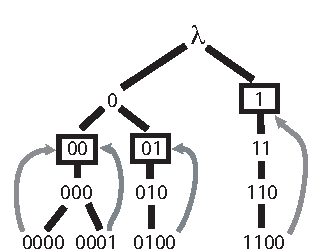
\includegraphics{pics/exthash-tree}
\caption{Reprezentace mno�iny $S$. Vrchol reprezentuj�c� prefix $0$, by ve
sv�m podstrom� m�l 3 prvky, co� je v�ce, ne� po�adujeme pomoc� hodnoty
$b$.}
\label{fig.hash.extern}
\end{figure}

Z obr. \ref{fig.hash.extern} plyne, �e hodnota $d(S) = 2$.
\end{priklad}

\begin{tvrzeni}
Plat�: Kdy� $d(s) = k$ a prvek $t$ m� stejn� prefix d�lky $k$ jako $s$, 
pak $d(s) = d(t)$. 
\end{tvrzeni}

Reprezentace: 
\begin{itemize}
\item adres��: ke ka�d�mu slovu $\alpha$ d�lky $d(S)$ je p�i�azena adresa 
str�nky, kter� obsahuje prvky $s \in S$, �e $h(s)$ m� prefix $\alpha$.
Tato slova d�lky $d(s)$ jsou lexikograficky uspo��d�na.
\item datov� ��st: str�nky s p�i�azen�mi prvky
\end{itemize}

\begin{priklad}
P��klad adres��e pro mno�inu $\{0000, 0001, 0100, 1001 \}$:

\vspace{5mm}

\begin{tabular}{lll}
00 & $\rightarrow$ & 0000, 0001 \\
01 & $\rightarrow$ & 0100 \\
\hline
10 & $\searrow$ & \\
11 & $\rightarrow$ & 1001 \\
\end{tabular}
\end{priklad}

\begin{pozn}
Up�esn�n� reprezentace str�nky (str�nek): \\
Prvek $s \in S$ je ulo�en na str�nce, kter� obsahuje v�echny prvky $t \in
S$ takov�, �e prefix $h(t)$ d�lky $d(s)$ bude je stejn� jako $h(s)$, tato st�nka
bude p�i�azena v�em slov�m $\alpha$ d�lky $d(S)$ takov�m, �e prefix $h(s)$ d�lky
$d(s)$ je prefix $\alpha$. \\
Pokud $\alpha$ neobsahuje ��dn� takov� prefix, tak je mu p�i�azena str�nka
NIL.
\end{pozn}

\subsection{Operace ACCESS}

viz algoritmus \ref{alg:exthash.access}

\begin{algorithm}[!htb]
\caption{ACCESS pro extern� ha�ov�n�}
\label{alg:exthash.access}
ACCESS(x)
\begin{enumerate}
\item Spo��t�me $h(x)$, nat�hneme adres��, nalezneme $d(S)$ a najdeme
str�nky odpov�daj�c� prefixu $h(x)$ d�lky $d(S)$
\item Nat�hneme odpov�daj�c� str�nku do pam�ti, zjist�me, zda obsahuje $x$ a
kdy� ano, provedeme po�adoven� �pravy.
\item Str�nku ulo��me zp�t na stejn� m�sto.
\end{enumerate}
\end{algorithm}

Operace ACCESS vy�aduje 3 p��stupy na extern� medium. (za p�edpokladu, �e
adres�� je tak� ulo�en na extern�m mediu a zab�r� jednu str�nku) 

Pro rychlou implementaci aktualiza�n�ch operac� je vhodn� m�t u ka�d�
str�nky ulo�eno informaci kolik je prvk� na str�nce.


\subsection{Operace INSERT}

viz algoritmus \ref{alg:exthash.insert}

% pozn: \mnote nesmi byt uvnitr prostredi algorithm
\begin{algorithm}[!htb]
\caption{INSERT pro extern� ha�ov�n�}
\label{alg:exthash.insert}
INSERT(x)
\begin{enumerate}
\item Spo��t�me $h(x)$, nat�hneme adres��, nalezneme $d(S)$ a nalezneme adresu
str�nky odpov�daj�c� prefixu $h(x)$ d�lky $d(S)$. (XXX odkud vezmu $d(S)$ ?)
% XXX \mnote{$d(S)$ vezmu odkud ?}
\item Nat�hneme do pam�ti odpov�daj�c� str�nku. kdy� v n� existuje $x$ 
$\rightarrow$ konec
\item Kdy� neobsahuje $x$ a m� m�n� prvk� ne� $b$, vlo��me $x$ do t�to str�nky
a ulo��me ji zp�tky na stejn� m�sto a aktualizujeme adres�� (po�ty prvk�
na str�nce)
\item Kdy� str�nka prvek $x$ neobsahuje a m� $b$ prvk�, str�nku rozd�l�me
(nalezneme nov� $d(s)$ pro $s$ z t�to str�nky i s p�idan�m $x$), str�nky 
ulo��me a aktualizujeme adres��.
\end{enumerate}
\end{algorithm}
\mnote{pokud je nov� nalezen� $d(s) \leq d(S)$, adres�� se zv�t�ovat nebude}

Operace INSERT vy�aduje 6 p��stup� na extern� medium.

\begin{pozn}
Roz�t�pen� str�nky nemus� nutn� znamenat zv�t�en� adres��e.
\end{pozn}

\begin{priklad}
\label{priklad:exthash.insert2}
Do mno�iny z p��kladu \ref{priklad:exthash.tree} vlo��me pomoc� operace
INSERT prvek 1111. Hodnota $d(1100) = 1$ se po vlo�en� prvku 1111
nezm�n�. Podstrom reprezentuj�c� prvky mno�iny $S$ s prefixem 11
bude m�t po vlo�en� prvku 1111 dva syny. (viz obr.
\ref{fig.hash.extern.ins})

\begin{figure}[!htb]
\centering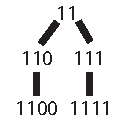
\includegraphics{pics/exthash-ins}
\caption{Podstrom reprezentuj�c� prvky mno�iny $S$ s prefixem 11 po
vlo�en� prvku 1111}
\label{fig.hash.extern.ins}
\end{figure}

Pokud vezmeme situaci danou po vlo�en� prvku 1111, bude adres�� vypadat
takto:

\vspace{5mm}

\begin{tabular}{lll}
00 & $\rightarrow$ & 0000, 0001 \\
\hline
01 & $\rightarrow$ & 0100 \\
\hline
10 & $\searrow$ & 	 \\
  & &  1001 \\
11 & $\nearrow$	& \\
\end{tabular}

\vspace{5mm}

Nyn� vlo��me prvek 0010. V tomto p��pad� dojde ke zv�t�en� adres��e:

\vspace{5mm}

\begin{tabular}{lll}
000 & $\rightarrow$ & 0000, 0001 \\
\hline
001 & $\rightarrow$ & 0010 \\
\hline
010 & $\rightarrow$ & 0100 \\
011 & $\nearrow$ & \\
\hline
100 & $\searrow$ & \\
101 & $\rightarrow$ &  1001, 1111 \\
110 & $\nearrow$ & \\
111 & $\nearrow$ & \\
\end{tabular}

\vspace{5mm}

Hodnota $d(S)$ je nyn� 3.
\end{priklad}


\subsection{Operace DELETE}

viz algoritmus \ref{alg:exthash.delete}

\begin{algorithm}[!htb]
\caption{DELETE pro extern� ha�ov�n�}
\label{alg:exthash.delete}
DELETE(x)
\begin{enumerate}
\item spo��t�me $h(x)$, nat�hneme adres��, nalezneme $d(S)$, nalezneme adresu
str�nky odpov�daj�c� prefixu $h(x)$ d�lky $d(S)$, zjist�me zda po odebr�n�
prvku $x$ m��e nastat spojov�n� str�nek a pokud ano, nalezneme adresu
str�nky, kter� se spoj� s na�� str�nkou
\item nat�hneme odpov�daj�c� str�nku do pam�ti, zjist�me zda obsahuje $x$,
pokud ne, tak konec
\item kdy� obsahuje $x$ a nem��e doj�t ke slou�en� str�nek, tak odstran�me
$x$, str�nku ulo��me na stejn� m�sto a aktualizujeme adres�� (po�ty prvk� na
str�nce)
\item kdy� obsahuje a dojde ke slu�ov�n�, pak odstran�me $x$, nat�hneme
druhou str�nku a str�nky slou��me, ulo��me novou str�nku a aktualizujeme
adres��.
\end{enumerate}
\end{algorithm}
\mnote{pro aktualizaci adres��e to mohou b�t 2 operace - na�ten� a
ulo�en�. z�ejm� proto, aby mohlo b�t sou�asn� pu�t�no v�c operac�.}

\begin{priklad}
Pro situaci z p��kladu \ref{priklad:exthash.insert} provedeme
DELETE(0100). V adres��i budou pak polo�ky 010 a 011 ukazovat na pr�zdnou
str�nku (NIL). Adres�� z�stal po t�to operaci stejn�.

Nyn� sma�eme prvek 0001.

\begin{figure}[!htb]
\centering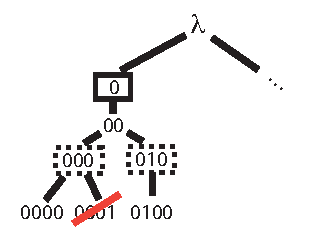
\includegraphics{pics/exthash-del}
\caption{��st stromu reprezentuj�c�ho mno�inu $S$ p�ed smaz�n�m prvku 0001}
\label{fig.hash.extern.del}
\end{figure}

Na obr. \ref{fig.hash.extern.del} je vid�t, �e po smaz�n� prvku 
0001 m��e b�t adres�� op�t zmen�en.

Po proveden� DELETE(0001) bude adres�� vypadat takto:

\vspace{5mm}

\begin{tabular}{lll}
000 & $\rightarrow$ & 0000, 0010 \\
001 & $\nearrow$ & \\
\hline
010 & $\rightarrow$ & NIL \\
011 & $\nearrow$ & \\
\hline
100 & $\searrow$ & \\
101 & $\rightarrow$ &  1001, 1111 \\
110 & $\nearrow$ & \\
111 & $\nearrow$ & \\
\end{tabular}

\vspace{5mm}

Nyn� m��eme prov�st zmen�en� adres��e na:

\vspace{5mm}

\begin{tabular}{lll}
00 & $\rightarrow$ & 0000, 0010 \\
01 & $\nearrow$ & \\
\hline
10 & $\rightarrow$ & 1100, 1111	 \\
11 & $\nearrow$	& \\
\end{tabular}

\vspace{5mm}

Tento adres�� m��eme je�t� zmen�it:

\vspace{5mm}

\begin{tabular}{lll}
0 & $\rightarrow$ & 0000, 0010 \\
\hline
1 & $\rightarrow$ & 1100, 1111 \\
\end{tabular}
\end{priklad}

\begin{pozn}
Pesimistick� odhad pro operaci DELETE je nejv��e 6 p��stup� na extern� 
medium.
\end{pozn}

\subsubsection{Aktualizace adres��e}

V posledn�m kroku DELETE se prov�d� aktualizace adres��e. 
Nejprve provedeme opraven� odkaz� na str�nky: pokud u sud�ho z�znamu v
adres��i dojde k vypr�zdn�n� str�nky, bude tam odkaz na NIL. pokud dojde k
vypr�zdn�n� u lich� str�nky, p�ehod� se odkaz na p�edchoz� (sudou)
str�nku.

Potom se testuje, zda jde adres�� zmen�it. Zmen�ov�n� prov�d�me tak
dlouho, dokud to jde.

\subsection{Reprezentace adres��e}

\begin{itemize}
\item reprezentovat jako posloupnost dvojic (adresa str�nky, po�et prvk� na
str�nce), kde $i$-t� dvojice je p�i�azen� $i$-t�mu slovu v lexikografick�m
uspo��d�n�.
\item zv�t�ov�n� adres��e znamen� zdvojen� prvk�
\item test na zmen�ov�n� adres��e - testujeme, zda adresa na lich�m m�st�
je stejn� jako adresa na n�sleduj�c�m sud�m m�st� - pokud ano, tak zmen��m
adres�� vymaz�n�m sud�ch �len� posloupnosti.
\end{itemize}

O�ek�van� zapln�n� str�nky p�i rovnom�rn�m rozlo�en� dat je 
$b \ln 2 \approx 0.69 b$

O�ek�van� velikost adres��e je $\frac{e}{b \ln 2} n^{1 + \frac{1}{b}}$ (p�i
rovnom�rn�m rozlo�en� dat)

\begin{pozn}
�len $n^{1 + \frac{1}{b}}$ nen� line�rn�, zde je probl�m, proto se to
nehod� pro mal� $b$.
\end{pozn}

\begin{tabular}{|l||l|l|l|l|}
\hline
b/n   	&$10^5$   &$10^6$ 	&$10^8$ 	&$10^{10}$    \\
\hline
2  	&$6.2*10^7$  &$1.96*10^8$	&$1.96*10^{11}$	&$1.96*10^{14}$ \\
10	&$1.2*10^5$  &$1.5*10^6$	&$2.4*10^8$	&$3.9*10^{10}$  \\
50	&$9.8*10^3$  &$1.0*10^6$	&$1.1*10^8$	&$1.2*10^{10}$  \\
100	&$4.4*10^3$  &$4.5*10^4$	&$4.7*10^6$	&$4.9*10^8$   \\
\hline
\end{tabular}

\vspace{5mm}

Jak je vid�t, pro $b = 2$ se to nehod�, adres�� je v�t�� ne� velikost dat.

\begin{pozn}
Kdy� pracujeme s velikost� $S$ kolem $10^{10}$, pak je vhodn�, aby 
$b \geq 100$. Pro v�t�� mno�iny $S$ mus� b�t $b$ v�t��.
\end{pozn}

% --------------------------------------------------------------------------
\section{Perfektn� ha�ov�n�}

Perfektn�m ha�ov�n�m mysl�me �lohu nal�zt pro danou pevnou mno�inu 
$S \subseteq U, |S| = n$ perfektn� ha�ovac� funkci, tj. funkci, kter� nem� na 
mno�in� $S$ kolize. Tato �loha nep�ipou�t� p�irozenou implementaci 
operace INSERT, proto�e p�idan� prvek m��e zp�sobit kolizi. 
Typick� p��klad pou�it� je tabulka kl��ov�ch slov kompil�toru.

\begin{defn}
Funkce $h: U \to \intrange{0}{m-1}$ je perfektn� pro $S$, kdy� je na S
prost� ($\forall x\neq y \in S$ plat� $h(x) \neq h(y)$).
\end{defn}

Za jak�ch podm�nek lze povolit INSERT? Mus� b�t m�lo
pravd�podobn�. Prvky nav�c se d�vaj� jinam a po jist� dob� se v�e
p�epo��t� do jedn� tabulky pro novou perfektn� ha�ovac� funkci.

Po�adavky na hledanou ha�ovac� funkci:
\begin{enumerate}
\item $h$ je perfektn� na $S$
\item $\forall x$ je $h(x)$ rychle spo�itateln�
\item $m$ ��dov� srovnateln� s $n$
\item zak�dov�n� $h$ vy�aduje m�lo prostoru
\end{enumerate}
Po�adavky 2) a 3) jdou proti sob�. A a� se n�m je poda�� skloubit,
budeme m�t probl�my s 4). A nav�c hled�n� $h$ potrv� dlouho.

% ..........................................................................
\subsection{Perfektn� ha�ovac� funkce do tabulky velikosti $n^2$}

Vyu�ijeme, co u� v�me o univerz�ln�m ha�ov�n�. Pro $k \in \intrange{1}{N-1}$ 
a pro pevn� $m$ definujme 
\begin{equation}
h_k(x) = ( kx \bmod N ) \bmod m, \quad\text{kde $N=|U|$ je prvo��slo.}
\end{equation}
Budeme hledat vhodn� $k$, $m$.
Definujme m�ru perfektnosti
\begin{equation}
d = \sum_{k=1}^{N-1} \sum_{x \neq y \in S} \delta_{h_k}(x,y)
\end{equation}
a pro $k \in \intrange{1}{N-1}$ polo�me
\begin{equation}
b_k(i) = |\{ x \in S : h_k(x) = i \}|
\end{equation}

Jednak plat�
\begin{align}
\label{bki2}
d & = \sum_{k=1}^{N-1} \left( \sum_{i=0}^{m-1} ( b_k(i) )^2 -n \right)\\
\intertext{a tak�}
d & = \sum_{x \neq y \in S} |\{ k : h_k(x)=h_k(y) \}|
	&&\text{prohozen�m sum}\\
\end{align}

Co znamen� $h_k(x) = h_k(y)$ pro $x \neq y$? N�sleduj�c� tvrzen� jsou
ekvivalentn�:
\begin{align*}
kx \bmod N & = ky \bmod N && \pmod m\\
k(x-y) \bmod N & = 0 && \pmod m\\
k(x-y) \bmod N & = r m && \text{pro } r \in 
% *ceil -> *floor (fakticka poznamka od Ladislava Proska
	\{ - \lfloor N/m \rfloor .. \lfloor N/m \rfloor \} - \{0\}, \\
\end{align*}
tedy
\[
d \leq \sum_{x \neq y \in S} 2 \frac Nm = \frac{2 n(n-1) N}m
\]
a dosazen�m do \eqref{bki2}, podle p�ihr�dkov�ho principu
\begin{equation}
\label{existsk}
\exists k : \sum_{i=0}^{m-1} ( b_k(i) )^2 \leq n + \frac{2 n(n-1)}m
\end{equation}

Pro speci�ln� velikosti tabulky dost�v�me dosazen�m do \eqref{existsk}:
\begin{align}
\label{3n}
&\text{Pro } m = n: 
&& \exists k \text{ naleziteln� v �ase }O(nN): 
\sum_{i=0}^{m-1} ( b_k(i) )^2 < 3n\\
\label{perf}
&\text{Pro } m = 1 + n(n-1): 
&& \exists k \text{ naleziteln� v �ase }O(nN):  
h_k \text{ je perfektn�} 
\end{align}

\begin{proof}
Prob�r�me v�echny mo�nosti pro $k$, t�ch je $O(N)$.
\begin{enumerate}
\item[\eqref{3n}]
Pro dan� $k$ spo��t�me $\sum ( b_k(i) )^2$ v �ase $O(n) = O(m)$.
\item[\eqref{perf}]
$\sum ( b_k(i) )^2 \leq n + \frac{2 n(n-1)}{1+ n(n-1)} < n + 2$.
Kdyby $h_k$ nebyla perfektn�, pak 
$\exists j : b_k(j) \geq 2$
a
$\sum ( b_k(i) )^2 \geq (n-2) 1^2 + 1 \cdot 2^2 = n + 2$,
spor.
P�i hled�n� $k$ ov���me perfektnost $h_k$ v �ase $O(n)$.
% zmatek s indexy u k (T. Matousek):
% Tohle by melo byt vporadku. k je jako scitaci index jen v (4.8) a (4.10)
% a dal uz ne.
% Ten soucet v d jde pres vsechny hashovaci funkce a jedna z nich je ta
% prava. Ja bych to tak nechal, je to ok. Staci smazat tu *.
\end{enumerate}
\end{proof}

Nyn� m�me perfektn� ha�ovac� funkci, kter� ale poru�uje po�adavek (3).
% ..........................................................................
\subsection{Perfektn� ha�ovac� funkce do tabulky velikosti $3n$}

Zkombinujeme oba v�sledky z p�edchoz� ��sti.
% --- nejprve prvn� funkc� ha�ujeme do tabulky velikosti $< 3n$

Podle \eqref{3n} nalezneme $k$ takov�, �e
$\sum ( b_k(i) )^2 < 3n$.

Pro ka�d� $i \in \intrange{0}{n-1}$ vezmeme mno�inu koliduj�c�ch prvk�
$S_i = \{ s \in S : h_k(s) = i \}$.
Ozna�me $n_i = |S_i|$.

Podle \eqref{perf} pro ka�d� $i$ nalezneme $k_i$ takov�, �e
pro $m_i = 1 + n_i(n_i-1)$ je $h_{k_i}$ perfektn� pro $S_i$.

Ka�dou zaha�ovanou mno�inu $S_i$ ulo��me ve v�sledn� tabulce od pozice
$d_i$: 
\[
d_i = \sum_{j=0}^{i-1}(1 + n_j(n_j-1)).
\]

Kone�n� definujme
\[
g(x) = d_i + h_{k_i}(x),\quad\text{kde } i = h_k(x),
\]
kter� je perfektn� a velikost tabulky je
\[
m = d_n = \sum_{j=0}^{n-1}(1 + n_j(n_j-1))
\leq \sum_{j=0}^{n-1} n_j^2
=  \sum_{j=0}^{n-1} (b_k(j))^2
< 3n
\]

Ov�em na zak�dov�n� t�to funkce pot�ebujeme hodn� pam�ti: 
nevad� n�m $d_i$, 
ale $k$ a ka�d� $k_i$ je velikosti $O(N)$, 
tedy pot�ebujeme $n \log_2 N$ bit�, co� odporuje na�emu po�adavku (4).
V dal��ch kroc�ch budeme zmen�ovat ��sla definuj�c� ha�ovac� funkci.
% ..........................................................................
\subsubsection{Podobn� funkce dan� ��slem velikosti $O(N)$}

\mnote{lep�� jm�na prom�nn�ch!}
Zvolme prvo��slo $p_1$ takov�, �e 
$1 +n(n-1) \leq p_1 \leq 1+ 2n(n-1)$. N�jak� takov� mus� existovat
(Bertrand�v postul�t: $\forall n>1 \exists$ prov��slo p, �e 
$n < p < 2n$).
Podle \eqref{perf} %TODO, mus�me dok�zat m \geq, co� m�rn� zatemn� dk.
$\exists k : h_k(x) = ( kx \bmod N) \bmod p_1$ 
je perfektn� na $S$.

Vytvo�me
\[
S_1 = \{ h_k(s) : s \in S\} \subset \intrange{0}{p_1 -1}
\]
a na $S_1$ aplikujme p�edchoz� sekci, kde $N = p_1$.

Dost�v�me ha�ovac� funkci $g_1$, kter�
\begin{itemize}
\item je perfektn� pro $S$
\item je spo�itateln� v �ase $O(1)$ 
\item ha�uje do tabulky $<3n$ 
\item je ur�ena 1 ��slem velikosti $O(N)$ \\
 \quad a $O(n)$ ��sly velikosti $O(n^2)$ 
\end{itemize}

% ..........................................................................
\subsubsection{Podobn� funkce dan� ��slem velikosti $O(n^2\log N)$}
Pro extr�mn� p��pady typu $N = 2^{10^6}$ je�t� postup vylep��me,
��m� zmen��me velikost ��sel k�duj�c�ch perfektn� ha�ovac� funkci 
na $O(\log N)$.

\begin{lemma}
\label{n2logN}
Pro ka�dou mno�inu $S \subseteq \intrange{0}{N-1}$ velikosti $n$ existuje
prvo��slo $p$ takov�, �e $f_{p}(x) = x \bmod p$ je perfektn� na
$S$ a $p = O(n^2 \log N)$.
\end{lemma}

Vyu�it�: pro $S$ najdeme prvo��slo $p_0$ velikosti $O(n^2 \log N)$
takov�, �e $f_{p_0}$ je perfektn� na $S$. Vytvo��me 
\[
S_0 = \{ f_{p_0}(s) : s \in S\} \subset \intrange{0}{p_0-1}
\]
a na $S_0$ aplikujme p�edchoz� postup, kde $N = p_0$.

Tedy pro ka�dou mno�inu $S$ velikosti $n$ existuje ha�ovac� funkce $f$, kter�
\begin{itemize}
\item je perfektn� pro $S$
\item je spo�itateln� v �ase $O(1)$ 
\item ha�uje do tabulky $<3n$ 
\item je ur�ena 2 ��sly velikosti $O(n^2 \log N)$ \\
 \quad a $O(n)$ ��sly velikosti $O(n^2)$ 
\end{itemize}

\begin{lemma}
\label{prvociselnidelitele}
Nech� $r$ je ��slo a $p_1, \ldots, p_q$ jsou v�echny jeho prvo��seln�
d�litele. Pak $q=O(\log r / \log\log r)$.
\end{lemma}
\begin{proof}
\begin{align*}
r & \geq \prod_{i=1}^q p_i\\
 & > q! \\
 & = \exp(\sum_{i=1}^q \ln i) \\
 & > \exp(\int_1^q \ln x \,dx) \\
 & \geq {\left( \frac qe \right)}^q \qquad\text{kde } \exp(x)=e^x
\end{align*}
Tedy
\mnote{skok}
\[
q \leq c \frac{\ln r}{\ln\ln r} \quad\text{pro vhodnou konstantu $c$.}
\]
\end{proof}
\begin{proof}[D�kaz lemmatu \ref{n2logN}]
P�edpokl�dejme $S = \{ x_1 < \ldots < x_n \}$.
Ha�ovac� funkce $f_t(x) = x \bmod t$ je perfektn� pr�v� kdy� $t$ je
nesoud�ln� s ��slem
\[
D = \prod_{i>j} (x_i - x_j) < N^{n^2}
\]
Podle \ref{prvociselnidelitele} je mezi prvn�mi $(c \ln D / \ln\ln D)+1$
prvo��sly alespo� jedno, kter� ned�l� $D$. V�me, �e $p_k = O(k \ln
k)$, tedy 
$(c \ln D / \ln\ln D) +1$-n� prvo��slo m� velikost
$O(\ln D) = O( n^2 \ln N)$.
\end{proof}
\mnote{nalezeni prvocisla $p_0$ vyzaduje cas $O(n^2\log N)$.}

% ..........................................................................
\subsection{GPERF}

Jin� konstrukce perfektn� ha�ovac� funkce je pou�ita v programu
{\tt gperf}. Distribuov�n pod GPL. 
Jeho n�vrh je pops�n v
Douglas C. Schmidt, "GPERF: A Perfect Hash Function Generator, "
in Proceedings of the 2nd C++ Conference, 
San Francisco, California, April 1990, USENIX, pp. 87--102.

\mnote{po��dnou bibliografii}
 �l�nek se d� st�hnout z 
\href
{http://citeseer.nj.nec.com/schmidt90gperf.html}
{citeseer}.

% --------------------------------------------------------------------------
\def\xx{% commented out
\section{Ha�ov�n� pro extern� pam�}

\mnote{Tohle u� Koubek nep�edn��}
Adres��.

MEMBER, INSERT, DELETE

O�ek�van� zapln�n� str�nky, po�et str�nek, velikost adres��e --- jen
citace, tabulka pro n�kter� ��sla.
}% commented out

% ==========================================================================
% Sou��st skript na Datov� struktury. Viz main.tex
\markright{$ $Id$ $}

\chapter{Trie}

% --------------------------------------------------------------------------
\section{Z�kladn� varianta}

Trie je rovinn� implementace slovn�ku.
M�me abecedu $\Sigma$ velikosti $k$. Universum jsou v�echna slova nad
$\Sigma$ d�lky pr�v� $l$ (nekone�nou mno�inu si nem��eme dovolit a
krat�� slova dopln�me zprava mezerami). Chceme reprezentovat mno�inu
slov $S \subseteq U$.

\begin{defn}
\emph{Trie} nad $\Sigma$ je kone�n� strom, jeho� ka�d� vnit�n�
vrchol m� pr�v� $k$ syn�, kter� jsou jednozna�n� ohodnoceny prvky $\Sigma$.
Ka�d�mu vnit�n�mu vrcholu trie odpov�d� slovo nad $\Sigma$ d�lky
nejv��e $l$: ko�enu
odpov�d� pr�zdn� slovo $\Lambda$; kdy� vrcholu $v$ odpov�d� slovo
$\alpha$, pak $v[a]$, synu $v$ ohodnocen�mu p�smenem $a$, odpov�d�
slovo $\alpha a$.
\end{defn}

\newcommand{\Nal}{\textrm{Nal}}
\begin{defn}
�ekneme, �e trie nad $\Sigma$ \emph{reprezentuje mno�inu} $S$, kdy�:
\begin{itemize}
\item List�m je p�i�azena boolovsk� funkce n�le�en� \Nal: $\Nal(t)$ je
  true pr�v� kdy� slovo, kter� odpov�d� listu $t$, je v $S$.
\item Kdy� $v$ je vnit�n� vrchol trie odpov�daj�c� slovu $\alpha$, pak
  existuje $\beta \in S$ takov�, �e $\alpha$ je prefix $\beta$.
\item Pro ka�d� slovo $\alpha \in S$ existuje v trie list odpov�daj�c�
  $\alpha$.
\end{itemize}
\end{defn}

% ..........................................................................
\subsection{Algoritmus MEMBER}

\begin{algorithmic}
\STATE \COMMENT {vyhled�n� $x = x_1 \dots x_l$}
\STATE $t := \text{ko�en}$
\STATE $i := 1$
\WHILE {$t \text{ nen� list}$}
        \STATE $t := t[x_i]$
        \STATE $i := i + 1$
\ENDWHILE
\STATE \COMMENT {test}
\STATE \textbf{return} $\Nal(t)$
\end{algorithmic}

% ..........................................................................
\subsection{Algoritmus INSERT}

\begin{algorithmic}
\STATE \COMMENT {vyhledej $x$}
\IF[trie nemus� b�t tak hlubok�, jak pot�ebujeme] {\textbf{not} $\Nal(t)$}
        \WHILE {$i \leq l$}
                \STATE vrcholu $t$ p�idej $k$ list� ohodnocen�ch
                p�smeny z $\Sigma$, jejich $\Nal := \textit{false}$
                \STATE $t := t[x_i]$
                \STATE $i := i + 1$
        \ENDWHILE
        \STATE $\Nal(t) := \textit{true}$
\ENDIF
\end{algorithmic}

% ..........................................................................
\subsection{Algoritmus DELETE}

\begin{algorithmic}
\STATE \COMMENT {vyhledej $x$}
\IF {$\Nal(t)$}
        \STATE $\Nal(t) := \textit{false}$
        \STATE $t := \text{otec } t$
        \STATE \COMMENT {oprav�me prefixovou podm�nku}
        \WHILE {v�ichni synov� $t$ jsou listy s $\Nal = \textit{false}$}
                \STATE zru� listy $t$
                \STATE $\Nal(t) := \textit{false}$
                \STATE $t := \text{otec } t$
        \ENDWHILE
\ENDIF  
\end{algorithmic}

Pou�ili jsme obrat $t := \text{otec } t$. To lze prov�st bu� tak, �e
se vrchol krom� sv�ch syn� odkazuje i na sv�ho otce a spot�ebuje tak
pam� nav�c, nebo se cesta z ko�ene do aktu�ln�ho vrcholu b�hem
sestupu ve stromu pamatuje na z�sobn�ku. Tento trik se pou��v� u 
v�ech stromov�ch struktur.

% ..........................................................................
\subsection{�asov� a pam�ov� slo�itost}

Jedna iterace cyklu zabere konstantn� �as. �as pro MEMBER je $O(l)$,
�as pro INSERT a DELETE je $O(l k)$. Pam�ov� slo�itost trie v nejhor��m
p��pad� je po�et
ulo�en�ch slov n�soben� d�lkou cesty a po�tem syn�, tedy $O(|S| l k)$.

\begin{pozn}
V p��pad�, kdy S obsahuje (skoro) v�echna slova d�lky l, tak m��e
m�t slo�itost jen O(|S|).
\end{pozn}

% --------------------------------------------------------------------------
\section{Komprimovan� trie}

M�jme $\Sigma = \{0,1,2\}$, $l=7$.
$S = \{0202011, 0202012, 0202021, 1212102, 1212111, 1212121, 1212122\}$.
Nekomprimovan� trie pro tuto mno�inu je na obr�zku \ref{fig:tries}.
Vid�me, �e p�smena na druh� a� p�t� pozici jsou v�dy stejn� a
p�edchoz� algoritmy se jimi mus� \uv{prokousat}. P�esn� 
�e�eno, prohl��en� vrcholu $v$, kter� m� jedin�ho 
syna, kter� nen� list s hodnotou $\Nal = \textit{false}$, nep�in�� 
��dnou kladnou informaci, proto�e mno�iny prvk� z $S$, 
kter� jsou reprezentov�ny vrcholy v podstromu otce $v$ a v podstromu 
vrcholu $v$ jsou stejn�. To vedlo k idei tyto vrcholy ze stromu vynechat a t�m 
zmen�it (komprimovat) trie.  
   
\begin{figure}
\centering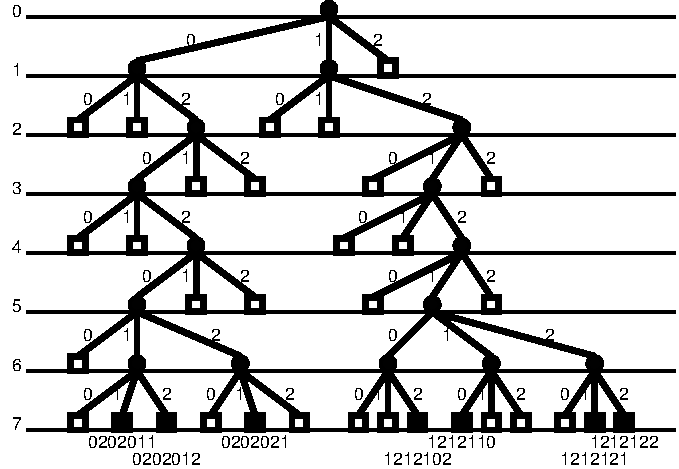
\includegraphics{pics/tries}
\caption{Nekomprimovan� trie}
\label{fig:tries}
\end{figure}

\newcommand{\uro}{\textrm{uroven}}
Ke ka�d�mu vrcholu $v$ p�id�me funkci $\uro(v)$ vyjad�uj�c� ��slo �rovn�,
ve kter� se $v$ nach�z� v p�vodn�m trie.
\newcommand{\slo}{\textrm{slovo}}
Ke ka�d�mu listu $v$ p�id�me funkci $\slo(v)$ --- slovo, kter� odpov�d� $v$.

Nyn� m��eme vynech�vat vrcholy podle n�sleduj�c�ho krit�ria: 
je-li $v$ vnit�n� vrchol a v�ichni jeho synov� krom� $w$ jsou listy s
$\Nal = \textit{false}$, pak $v$ vynech a za�a� $w$ na jeho m�sto. Tento proces 
opakujeme dokud trie obsahuje n�jak� vnit�n� vrchol, jeho� v�ichni synov� 
s v�jimkou jednoho jsou listy, pro n� $\Nal = \textit{false}$. V�imn�te si, �e 
ka�d� vnit�n� vrchol m� pr�v� $k$ syn�, kter� jsou v jednozna�n� 
korespondenci s p�smeny abecedy $\Sigma$.

% ..........................................................................
\subsection{MEMBER}

Viz algoritmus \ref{alg:trie.k.mem}

\begin{algorithm}[!htb]
\caption{MEMBER pro komprimovan� trie}
\label{alg:trie.k.mem}
\begin{algorithmic}
\STATE \COMMENT {vyhled�n� $x$}
\STATE $t := \text{ko�en}$
\WHILE {$t \text{ nen� list}$}
        \STATE $i := \uro(t) + 1$
        \STATE $t := t[x_i]$
\ENDWHILE
\STATE \COMMENT {test}
\STATE \textbf{return} $\Nal(t) \land \slo(t) = x$
\end{algorithmic}
\end{algorithm}

zde \mnote{n�co chyb�}
% ..........................................................................
\subsection{INSERT}

Viz algoritmus \ref{alg:trie.k.ins}

\begin{algorithm}
\caption{INSERT pro komprimovan� trie}
\label{alg:trie.k.ins}
\begin{algorithmic}
\STATE \COMMENT {vyhledej $x$}
\IF {$\Nal(t) \land \slo(t) = x$}
	\STATE \COMMENT {Trie u� obsahuje $x$, ned�lej nic.}
\ELSE
        \IF {$\slo(t) = x$}
		\STATE \COMMENT {Trie obsahuje spr�vn� list,
		pouze nastav p��znak. Nap�. "0202010"}
                \STATE $\Nal(t) := \textit{true}$
	\ELSE
		\STATE \COMMENT {Bude pot�eba vlo�it nov� list.}
		\STATE \COMMENT {Najdi, kam ho p�ipojit.}
                \STATE $\alpha$ := nejdel�� spole�n� prefix slov
		$x$ a $\slo(t)$. D�lku $\alpha$ ozna�me $|\alpha|$.
                \STATE $v$ := vrchol na cest� z ko�ene do $t$ takov�,
                �e $\uro(v)$ je nejv�t��, kter� je $\leq |\alpha|$
                \IF {$\uro(v) = |\alpha|$}
                        \STATE \COMMENT {$v$ je otec nov�ho listu}
		\ELSE[$\uro(v) < |\alpha|$]
                        \STATE \COMMENT {Bude pot�eba vytvo�it
			otce nov�ho listu}
                        \STATE $a$ := $\uro(v)+1$-n� p�smeno $\alpha$
                        \STATE $u := v[a]$
                        \STATE \COMMENT {Mezi $v$ a $u$ vytvo� nov�
			vnit�n� vrchol odpov�daj�c� slovu $\alpha$}
                        \STATE $w$ := nov� vrchol, $\uro(w) := |\alpha|$
                        \STATE $v[a] := w$
                        \STATE $c$ := $|\alpha|+1$-n� p�smeno $\slo(t)$
                        \STATE $w[c] := u$
                        \FORALL {$b \in \Sigma, b \neq c$}
                             \STATE $z$ := nov� vrchol, $\uro(z) := |\alpha|+1, \Nal(z) := \textit{false}, \slo(z) := \alpha b$, 
                             \STATE $w[b] := z$
                        \ENDFOR
                        \STATE $v := w$
                \ENDIF
		\STATE \COMMENT {Spr�vn�mu listu p�i�a� $x$}
		\STATE $d$ := $|\alpha|+1$-n� p�smeno $x$
                \STATE $s := v[d]$
                \STATE $\uro(s) := l, \Nal(s) := \textit{true}, \slo(s) := x$
        \ENDIF
\ENDIF
\end{algorithmic}
\end{algorithm}

% ..........................................................................
\subsection{DELETE}

Viz algoritmus \ref{alg:trie.k.del}

\begin{algorithm}[!htb]
\caption{DELETE pro komprimovan� trie}
\label{alg:trie.k.del}
\begin{algorithmic}
\STATE \COMMENT {vyhledej $x$}
\IF {$\Nal(t) \land \slo(t) = x$}
        \STATE $u$ := otec $t$
        \STATE $i := \uro(u)$
        \STATE $\Nal(t) := \textit{false}$
        \STATE $\uro(t) := i+1$, $\slo(t)$ := prefix slova $x$ d�lky $i+1$
        \STATE \COMMENT {vrchol $u$ m� alespo� jednoho syna, kter� nen� list s $\Nal = \textit{false}$}
        \IF {v�ichni synov� $u$ krom� syna $w$ jsou listy s $\Nal = \textit{false}$}
                \STATE $v$ := otec $u$
                \STATE sma� $u$ a v�echny syny $u$ krom� $w$
                \STATE $j := \uro(v) + 1$
                \STATE $v[x_j] := w$ (tj. $x_j$-t� syn v je w)
        \ENDIF
\ENDIF  
\end{algorithmic}
\end{algorithm}

% ..........................................................................
\subsection{�asov� a pam�ov� slo�itost}

Pam�ov� slo�itost takto komprimovan�ch trie je $O(nk)$, kde 
% oprava by Ladislav Prosek O(nl + kl) -> O(nk)
$n$ je velikost reprezentovan� mno�iny. (maxim�ln� $n-1$ vnit�n�ch vrchol�,
ka�d� s polem d�lky $k$).
�asov� slo�itost operace MEMBER je v nejhor��m
p��pad� $O(l)$, pro INSERT a DELETE je to $O(l+k)$. 
(m��e b�t nutn� p�idat/odebrat jeden vnit�n� vrchol).
% oprava slozitosti v nejhorsim pripade by Ladislav Prosek 

V pr�m�rn�m p��pad� (za p�edpokladu rovnom�rn�ho
rozlo�en� vstupn�ch dat) je to o�ek�van� hloubka trie. Tu
te� spo��t�me.

Nech�
\[
q_d = \pr(\text{trie m� hloubku alespo� $d$})
\]
O�ek�van� hloubka trie reprezentuj�c� $n$ slov je
\[
E_n = \sum_{d=0}^\infty d (q_d - q_{d+1}) = \sum_{d=0}^\infty q_d
\]
Kdy� funkce $\text{pref}_{d-1}$, p�i�azuj�c� slovu 
$\alpha$ jeho prefix d�lky $d-1$, je na mno�in� $S$ prost�,
pak trie reprezentuj�c� mno�inu $S$ m� hloubku nejv��e $d$.
Spo��t�me po�et mno�in o velikosti $n$, na nich� je funkce $\text{pref}_{d-1}$ 
prost�. Tyto mno�iny z�sk�me tak, �e vybereme $n$ prefix� d�lky $d-1$
a ka�d� dopln�me v�emi sufixy d�lky $l-d+1$. Proto t�chto mno�in je
\[
\binom{k^{d-1}}{n} k^{n (l-d+1)}.
\]
Proto�e v�ech podmno�in velikosti $n$ je $\binom{k^l}{n}$ dost�v�me, �e 
\begin{align*}  
q_d 
 &\leq 1 - \frac{\binom{k^{d-1}}{n} k^{n (l-d+1)}}{\binom{k^l}{n}}\\
 &\leq 1 - \frac{k^{d-1}(k^{d-1}-1)\dots(k^{d-1}-(n-1)) k^{n(l-d+1)}}{k^{ln}}\\
 &   = 1 - \prod_{i=0}^{n-1} \left( 1 - \frac{i}{k^{d-1}} \right) \\
 &\leq 1 - \exp\left( \frac{-n^2}{k^{d-1}} \right)\\
 &\leq \frac{n^2}{k^{d-1}},
\end{align*}
pon�vad�
\begin{align*}
                  \prod_{i=0}^{n-1}    \left( 1 - \frac{i}{k^{d-1}} \right)
 &   = \exp\left( \sum_{i=0}^{n-1} \ln \left( 1 - \frac{i}{k^{d-1}} \right)
	   \right)\\
 &\geq \exp\left(         \int_0^n \ln \left( 1 - \frac{i}{k^{d-1}} \right)
	   \right)\\
 &   = \exp\left( \frac{-n^2}{k^{d-1}} \right),
\end{align*} 
(u�ijte integr�ln� kriterium a substituci $x = k^{d-1}(1-t)$) a 
$e^x - 1 \geq x$ (odtud $1 - e^x \leq -x$). Tedy pro $c = 2\lceil\log_kn\rceil$ 
dost�v�me
\begin{align*}
E_n
 & = \sum_{d=1}^cq_d + \sum_{d=c+1}^{\infty}q_d\\
 &\leq c + \sum_{d=c}^{\infty}\frac{n^2}{k^d}\\
 &\leq 2\lceil\log_kn\rceil +
		\left( \frac{n^2}{k^c} \right) \sum_{d=0}^{\infty} k^{-d}\\
 &\leq 2\lceil\log_kn\rceil + \frac{1}{1-1/k}\\
 & = 2\lceil\log_kn\rceil + \frac{k}{k-1}.
\end{align*}

Tedy o�ek�van� �as operace MEMBER je $O(log_k(n))$ ($O(\frac{\log n}{\log
k})$)
a $O(log_k(n) + k)$ pro INSERT a DELETE
\mnote{L.Pro�ek: Mo�n� v t� o�ek�van� slo�itosti by �lo +k zanedbat, ale
ne na z�klad� toho tvrzen�, kter� dokazuje jen o�ek�vanou hloubku}
pro komprimovan� trie (za p�edpoklad� rovnom�rn�ho rozlo�en� vstupn�ch dat) 
Zde parametr $k$ vyjad�uje vztah mezi prostorov�mi 
a �asov�mi n�roky.

% . . . .. . . .. .. .. . .  . .. .. .. . . ..  ..  .... . . .. . .. . .
% nasledujici sekci (jeste kompr. trie atd.) dopsal Vladimir Kotal, 2003

\begin{algorithm}[!htb]
	\caption{INSERT pro komprimovan� trie, analogie \ref{alg:trie.k.ins} (verze Koubek 2002)}
\label{alg:trie.k.ins_unk}
\begin{algorithmic}
\STATE INSERT($x=x_1, ..., x_l$)
\STATE t $\leftarrow$ ko�en
\WHILE {t neni list}
  \STATE i $\leftarrow$ hladina(t), t $\leftarrow$ $(a_{i+1})$-n� syn t
\ENDWHILE
\IF {prvek(t) neni prefix x}
  \STATE beta = nejvetsi spolecny prefix x a prvek(t)
  \STATE beta a = prefix alfa
  \STATE beta b = prefix prvek(t)
  \STATE while $hladina(t) > |beta|$ do t $\leftarrow$ otec(t) done
  \IF {hladina(t) < |beta|}
    \STATE vytvo��me nov� vrchol w, jeho� synov�, krom� b-t�ho syna budou listy s
    \STATE funkcemi Nal = false
    \STATE prvek(t) = beta + oznaceni syna
    \STATE $hladina(w) = |beta|, beta = (a_1, ..., a_i)$
    \STATE necht $v = a_{hladina(t) + 1}$ - t� syn t, b-ty syn w je v
    \STATE $w = a_{hladina(t)+1}$-t� syn t
  \ENDIF
  \STATE z $\leftarrow$ a-ty syn t, Nal(z) = true, prvek(z) = x
\ELSE
  \STATE Nal(t) = true, prvek(t) = x
\ENDIF
\end{algorithmic}
\end{algorithm}

\mnote{XXX dalsi neznamy algoritmus z prednasky 2002}
\begin{algorithm}[!htb]
\caption{DELETE pro komprimovan� trie (?)}
\label{alg:trie.k.del_unk}
DELETE($x=x_1, ..., x_l$)
\begin{algorithmic}
\STATE t $\leftarrow$ ko�en
\WHILE {t neni list}
  \STATE i $\leftarrow$ hladina(t), t $\leftarrow$ $(a_{i+1}$-ni syn t
\ENDWHILE
\IF {Nal(t) = true a prvek(t) = j} 
  \STATE Nal(t) = false
  \STATE v $\leftarrow$ otec(t)
  \STATE prvek(t) $\leftarrow$ prefix prvek(t) o d�lce hladina v+1
  \IF {vsichni synove vrchovlu v az na jednoho jsou listy s Nal = false}
    \STATE w $\leftarrow$ syn(v), ktery je bud list s Nal(w) = true nebo neni list
    \STATE necht v je a-t� ($a_i$-ty ???) syn sv�ho otce, v sma�eme a sma�eme
    \STATE v�echny syny $v \neq w$
    \STATE w $\leftarrow$ a-t� ($a_i$-t� ???) syn otce v
  \ENDIF
\ENDIF
\end{algorithmic}
\end{algorithm}


\section{Je�t� komprimovan�j�� trie}

% XXX dopsat !
P�: \\
m�jme n�seduj�c� komprimovan� trie: \\
% XXX obr.
\mnote{tady chyb� obr�zek}

a jeho matici: \\

\begin{tabular}{|l|l|l|l|}
\hline
 & 0 & 1 & 2 \\
\hline
root & NIL & a & b \\
a & 102 & NIL & c \\
b & 210 & 211 & 212 \\
c & 120 & 121 & NIL \\
\hline
\end{tabular}

Chceme se zbavit polo�ek NIL v matici reprezentuj�c� trie. Dal�� komprese
dos�hneme pomoc� vektor� hod (vektor hodnot) a rd. Tyto vektory budou
reprezentovat p�vodn� matici.

\mnote{co znamena rd ?}

\subsection{Popis $A$ a $rd$}

Zp�t k na�emu p��kladu: \\
\par
I. \\
\begin{tabular}{|lllllll|}
\hline
hod & 210 & 211 & 212 & 120 & 121 & NIL \\
rd & root & a & b & c & & \\
 & & & 0 & 3 & & \\
\hline
\end{tabular}
\par

II. \\
\begin{tabular}{|lllllllllll|}
\hline
hod & 210 & 211 & 212 & 120 & 121 & a & b & 102 & NIL & c \\
rd & root & a & b & c & & & & & & \\
 & 4 & 7 & 0 & 3 & & & & & & \\
\hline
\end{tabular}

\par
��dek i za��n� na m�st� rd(i) a mus� b�t spln�na podm�nka: \\
Kdy� $M_{i,j} \neq NIL \neq M_{i',j'}$, pak $rd(i) + j \neq rd(i') + j'$ \\
Kdy� na m�st� hod chceme zapsat prvek $\neq NIL$ a NIL, pak zap��eme prvek
$\neq NIL$.


\subsection{Algoritmus pro hled�n� rd a hod}
Nech� M je matice typu r x s, m� m v�znamn�ch m�st $\neq$ NIL.
\begin{itemize}
\item pro ka�d� ��dek nalezneme po�et m�st $\neq$ NIL
\item set��d�me ��dky Bucketsortem, tak �e r�dky s v�t��m po�tem m�st $\neq$ NIL
  p�edch�zej� ��dky s men��m po�tem m�st $\neq$ NIL
\item proch�z�me ��dky v dan�m set��d�n� a pro ka�d� ��dek i nalezneme
  nejmen�� ��slo rd(i), �e nedoch�z� ke kolizi s p�edchoz�mi ��dky (tj.
  kdy� $M_{i',j'} \neq NIL \neq M_{i,j}$) a ��dek i' byl za�azen, pak
  $rd(i) + j \neq rd(i') + j'$.
  Pak $M_{i,j} \neq NIL$ je ulo�eno ve vektoru hod na m�st� rd(i)+j.
\end{itemize}

m(l) - po�et m�st $\neq$ NIL v ��dc�ch s po�tem m�st $\geq l+1 \neq NIL$.

\begin{theorem}
Kdy� $m(l)(l+1) \leq m$ pro ka�d� l, pak $rd(i) < m$ pro ka�d� ��dek i a
algoritmus vy�aduje �as O(rsm).
\end{theorem}

\begin{proof}
P�edpokl�dejme, �e hled�me rd pro ��dek i, kter� m� l m�st $\neq NIL$. \\
ve vektoru hod je obsazeno m�n� ne� m(l-1) m�st. \\ 
zkou��me rd(i)=1,2,... \\
rd(i) = 1,2,... je zak�zan�, kdy� vznikne kolize. \\
tj. $\exists$ ��dek i' p�edch�zej�c� a $\exists j,j'$ takov�, �e $M_{i',j'} \neq
NIL \neq M_{i,j}$ a platilo by $rd(i') + j' = rd(i) + j$.
$\rightarrow$ t�chto mo�nost� je $< lm(l-1) \leq m$. \\
O(rs) - zjist�me pro ka�d� ��dek po�et m�st $\neq NIL$. \\
O(m+r) - t��d�n� Bucketsortem \\
O(mrs) - krok 2
\end{proof}

P�:
jedna mo�nost

% XXX obr. matice
M = 

$\rightarrow$ budeme m�t moc ��dk� - nevhodn�

P�:\\

\begin{tabular}{|l|lll|}
\hline
M & 0 & 1 & 2 \\
\hline
root & NIL & a & b \\
a & 102 & NIL & c \\
b & 210 & 211 & 212 \\
c & 120 & 121 & NIL \\
\hline
\end{tabular}

\begin{tabular}{|l|llllllllll|}
\hline
rd  & root & a   & b   & c   &     &   &   &     &     &   \\
    &    4 & 7   & 0   & 3   &     &   &   &     &     &   \\
hod & 210  & 211 & 212 & 120 & 121 & a & b & 102 & NIL & c \\
\hline
\end{tabular}

\begin{tabular}{|l|lll|}
\hline
M' & 0 & 1 & 2 \\
\hline
b & 210 & 211 & 212 \\
c & 120 & 121 & NIL \\
root & NIL & a & b \\
a & 102 & NIL & c \\
\hline
\end{tabular}

(p�ehodili jsme pouze ��dky)

\begin{tabular}{|lll|}
\hline
210 & NIL & NIL \\
120 & 211 & 212 \\
NIL & 121 & NIL \\
102 & a & b \\
NIL & NIL & c \\
\hline
\end{tabular}


\subsection{Vertik�ln� posun sloupc�}

cd - vektor sloupcov�ho posunut�, slou�� k z�pisu transformace

\begin{tabular}{|l|lll|}
\hline
 & 0 & 1 & 2 \\
cd & 0 & 1 & 2 \\
\hline
\end{tabular}
\par

\begin{tabular}{|l|lllll|}
\hline
 & 0 & 1 & 2 & 3 & 4 \\
rd & 6 & 0 & 6 & 3 & 6 \\
\hline
\end{tabular}
\par

\begin{tabular}{|l|lllllllll|}
\hline
hod & 120 & 211 & 212 & 102 & a & b & 210 & 121 & c \\
\hline
\end{tabular}
\par

Jak najdeme nazp�tek m�sta ? Plat�, kdy� $M_{i,j} \neq NIL$, pak
$hod(rd(i+cd(j)+j)) = M_{i,j}$
\mnote{je ten vzorec spr�vn� ?}

\par
{\em zna�en�:} 
\begin{itemize}
\item f(-,-) je fce dvou prom�nn�ch 
\item $B_j$ matice posunut�ch prvn�ch sloupc� 
\item $m_j$ po�et m�st $\neq NIL$ v $B_j$ 
\item $m_j(l)$ po�et m�st $\neq NIL$ v ��dc�ch matice $B_j$, kter� maj� aspo� l+1 m�st $\neq NIL$
\end{itemize}
\par

Budeme cht�t, aby $\forall j \forall l$ platilo $m_j(l) \leq
\frac{m}{f(l,m_j)}$. \\
Okrajov� podm�nky na f: f mus� spl�ovat:
\begin{itemize}
\item $\forall$ l plat� $f(l,m) \geq l+1$
\item$\forall$ j plat� $f(0,m_j) \leq \frac{m}{m_j}$
\end{itemize}

\subsubsection{Algoritmus na posunut� sloupc�}

1) pro ka�d� sloupec v po�ad� 0,1,... nalezneme nejmen�� cd(j) takov�, aby
matice $B_j$ spl�ovala $\forall l$ $m_j(l) \leq \frac{m}{f(l,m_j)}$
(ka�d� sloupec posunujeme dokud nespl�uje podm�nku) \\
Na z�skanou matici $B = B_s$ pak pou�ijeme p�edchoz� algoritmus. \\
Plat� $m(l) = m_s(l) \leq \frac{m}{f(l,m)} \leq \frac{m}{l+1}$. \\
Hled�me hodnotu cd(j) a p�edp., �e pro n�jakou hodnotu cd(j) nen� spln�na
podm�nka pro l, tj. plat� $m_j(l) > \frac{m}{f(l,m)}$
... platila pro $B_{j-1}, tj. m_{j-1}(l) \leq \frac{m}{f(l,m_{j-1})}$
\par
Z toho plyne $m_j(l) - m_{j-1}(l) > \frac{m}{f(l,m_j)} -
\frac{m}{f(l,m_{j-1}}$.
\par

Jak roste ��slo $m_j(l)$ ? 
\begin{enumerate}
\item v matici $B_{j-1}$ existuje ��dek s aspo� l+1 m�sty $\neq NIL$ a s t�mto
��dkem se st�etne m�sto $\neq NIL$ (v j-t�m sloupci $\leftarrow
m_{j-1}(l)$
vzroste o 1)
\item v matici $B_{j-1}$ existuje ��dek s l m�sty $\neq NIL$ a s t�mto ��dkem
se st�etne m�sto $\neq NIL$ v j-t�m sloupci. Pak $m_{j-1}(l)$ vzroste o l+1.
\end{enumerate}

st�et - ��dek v $B_{j-1}$ s aspo� l m�sty $\neq NIL$ a m�sto $\neq NIL$ v j-t�m
sloupci. Aby nebyla spln�na podm�nka pro l, mus� b�t po�et st�et� pro danou hodnotu cd(j)
b�t aspo� 
$$\frac{\frac{m}{f(l,m_j)} - \frac{m}{f(l,m_{j-1})}}{l+1}$$
\par
V matici $B_{j-1}$ je nejv��e $\frac{m_{j-1}(l-1)}{l} \leq \frac{m}{l
f(l-1,m_{j-1}}$ ��dk� s aspo� l m�sty $\neq NIL$, v j-t�m sloupci je $m_j -
m_{j-1} m�st \neq NIL$. \\
\par

Podm�nka pro l m��e zak�zat nejv��e 
\begin{multline}\bigparens
\frac{ \frac{m(m_j - m_{j-1})}{l f(l-1,m_{j-1}} }
  { \frac{ \frac{m}{f(l,m_j} - \frac{m}{f(l,m_{j-1}} }{l+1} } 
\text{ hodnot cd} = 
\frac{l+1}{l} \frac{((m_j - m_{j-1})}{\frac{f(l.m_{j-1})}{f(l,m_j)} - 1}
  \frac{f(l.m_{j-1})}{f(l,m_{j-1})}
\end{multline}
\par

Sta�� n�m s��tat p�es hodnoty l takov�, �e \\
$m m_{j-1}(l) \leq l+1$ tj. p�es 
$l \leq l_0 = min\{l; \frac{m}{f(l,m_{j-1}} < l\}$, \\
$m_{j-1}(l) \leq \frac{m}{f(l,m_{j-1})} \leq l+1$.

Celkov� po�et zak�zan�ch hodnot cd je men�� ne� 
\begin{multline}
\label{odh-zak-hodnot}\bigparens
\sum_{l=0}^{l_0} \frac{l+1}{l} \frac{(m_j - m_{j-1})}{
\frac{f(l,m_{j-1}}{f(l,m_j)} - 1} \frac{f(l,m_{j-1}}{f(l-1,m_{j-1}}
\end{multline}

Zvol�me $f(l,m_j) = 2^{l(2 - \frac{m_j}{m})}$ \\
\mnote{"mystika"}
f spl�uje okrajov� podm�nky
$f(l,m) = 2^l \geq l+1 \forall l=0,1,...$ \\
$f(0,m_j) = 1 \leq \frac{m}{m_j} \forall j=0,1,...,s$

dosad�me do odhadu \ref{odh-zak-hodnot}
a dostaneme 

\begin{multline}
\sum_{l=1}^{l_0} 
  \frac{l+1}{l} 
  \frac
    {(m_j - m_{j-1})}
    { 2^{l ( \frac{m_j}{m} - frac{m_{j-1}}{m} ) }}
  2^{( 2 - \frac{m_{j-1}}{m} )} \leq \\
\text{vyu�ijeme, �e $2^x - 1 \geq x ln(2)$} \\
\sum_{l=1}^{l_0} 
  \frac{l+1}{l} 
  \frac{(m_j - m_{j-1})}{l( \frac{m_j}{m} - frac{m_{j-1}}{m} )} 4 = \\
\frac{4m}{ln(2)} \sum_{l=1}^{l_0} 
  \frac{l+1}{l^2} = \frac{4m}{ln(2)} (\sum_{l=1}^{l_0} \frac{1}{l} +
  \sum_{l=1}^{l_0} \frac{1}{l^2}) \leq \\
\text{integr�ln� kriterium} \\
\frac{4m}{ln(2)} (1 + ln(l_0)) + \frac{\pi^2}{6} \leq 4m log_2(l_0) +
15.3m \\
\text{odhadneme $l_0$: } 
l_0 = min\{l; \frac{m}{f(l,m_{j-1}} < l\} \rightarrow l_0 < log(m) \\
\text{pak } \leq 4m log(log(m)) + 15.3m
\end{multline}

Cel� algoritmus spo��t� ulo�en� matice M typu r x s do vektor�  \\
cd - dimenze s, \\
rd - dimenze $4m log(log(m)) + 15.3m + r$, \\
hod dimenze m+s, \\
p�itom hodnoty $cd(j) < 4m log(log(m)) + 15.3m$ a $rd(i) < m$.
\par
�as pot�ebn� k v�po�tu je $O(sr(m loglog(m))^2)$, kde m je po�et m�st $\neq
NIL$ v matici M.

\subsection{�sporn� ulo�en� ��dk�ho vektoru}

M�me vektor v dimenze $n \cdot d$ a $i_0 < i_1 < ... < i_{t-1}$ jsou v�echny
indexy i takov�, �e $v(i) \neq 0$. \\
Vytvo��me vektor cv dimenze t, $cv(j)=v(i_j)$. \\
N� �kol - pro dan� l zjistit, zda $l = i_j$ a p��padn� nal�zt toto j. \\
base - dimenze m

${\rm base(j) = }$
% \left 
$\Bigl\{$
\begin{tabular}{lll}
-1 & kdy� & $i_k$ {\tt div} $d \neq j \forall k=0,1,...,t-1$ \\
$min\{l; i_l div d = j\}$ & kdy� & $\exists l$, �e $i_l$ {\tt div} $d = j$ \\
\end{tabular}
% \right. 

vektor offset - dimenze n x d \\
${\rm offset(j,k) =}$
% \left 
$\Bigl\{$
\begin{tabular}{lll}
-1 & kdy� & $i_l \neq jd+k$ $\forall l = 0,1,...,t-1$ \\
$l-base(j)$ & kdy� & $i_l = jd+k$ \\
\end{tabular}

\mnote{jd+k ... z�pis v d-�kov� soustav�}

vektor off(j) = $\sum_{k=0}^{d-1}(offset(j,k) + 1)(d+1)^k$ \\
off je dimenze n \\
pot�ebujeme base(dim n), off (dim n) \\
smyslupln� kdy� $d << n$ a $t < n$ (nap�. $d = log(log(n))$)

pro dan� i - nalezen� hodnoty v(i)
kdy� base(i {\tt div} d) = -1, pak v(i) = 0  \\
base(i {\tt div} d) $\neq -1$, pak k = i {\tt mod} d \\
j = i div d \\
l = off(j) {\tt div} $(d+1)^k$ \\
l = l {\tt mod} (d+1) \\
l = l - 1 + base(j) \\
v(i) = cv(l) \\

Lze pou��t pro mal� t a $(d+1)^d$ v rozsahu velikosi registru - vhodn� nap�.
pro $d \approx log(log(n))$.

P�.:
v = 
\begin{tabular}{|l|l|l|l|}
\hline
0 1 0 & 1 0 1 & 0 0 0 & 0 0 1 \\
\hline
      0  &     1 &      -1 &    3 \\
\hline
\end{tabular}

$i_0$ = 1, $i_1$ = 3, $i_2$ = 5, $i_3$ = 11, d = 3 \\

cv = 
\begin{tabular}{|l|l|l|l|}
\hline
v(1) & v(3) & v(5) & v(11) \\
\hline
\end{tabular}

base =
\begin{tabular}{|l|l|l|l|}
\hline
0 & 1 & -1 & 3 \\
\hline
\end{tabular}

\begin{tabular}{|l|llll|}
\hline
offset & 0 & 1 & 2 & 3 \\
\hline
0 & -1 & 0 & -1 & -1 \\
1 & 0 & -1 & -1 & -1 \\
2 & -1 & 1 & -1 & 0 \\
\hline
\end{tabular}

3. sloupec tabulky offset repr. nuly \\
off = 
\begin{tabular}{|l|l|l|l|}
\hline
4 & 33 & 0 & 16 \\
\hline
\end{tabular}

$off(7) = (offset(1,0) + 1)4^0 + (offset(1,1) + 1)4^1 + (offset(1,2) +
1)4^2$
$off(1) = 1 + 0 + 2\cdot4^2 = 33$


% ==========================================================================
% Sou��st skript na Datov� struktury. Viz main.tex
\markright{$ $Id$ $}

\chapter{Uspo��dan� pole}

% --------------------------------------------------------------------------
\section{Un�rn�, bin�rn� a interpola�n� vyhled�v�n�}
% \mnote{Napsal Pavel Machek}
% pavel@ucw.cz

Uspo��dan� pole je datov� struktura, kter� vznikne z pole jeho
set��d�n�m. Jedin� operace, kter� se na n� d� (rozumn� rychle)
prov�d�t, je MEMBER.

M�jme slovn�k $S$ ulo�en� jako pole prvk� tak, �e $s[i] < s[i+1]$.

\begin{algorithm}
\caption{MEMBER pro uspo��dan� pole}
\label{alg:bin.member}
\begin{algorithmic}
\STATE \COMMENT {vyhled�n� hodnoty $x$ mezi $s[i] \dots s[j]$}
\STATE \COMMENT {odpov�� ANO, kdy� $\exists h : i \leq h \leq j \land s[h]=x$}
\STATE $d := i$ \COMMENT {aktu�ln� doln� a horn� odhad}
\STATE $h := j$
\STATE $\<next> := f(d, h)$
	\COMMENT { P�edpokl�d�me, �e $d \leq f(d,h) \leq h$ }
\WHILE {$s[\<next>] \neq x \land d < h$}
	\IF {$s[\<next>] < x$}
		\STATE $d := \<next> + 1$
	\ELSE
		\STATE $h := \<next> - 1$
	\ENDIF
        \STATE $\<next> := f(d, h)$
\ENDWHILE
\STATE \COMMENT {�ekni ANO pokud $s[\<next>] = x$, jinak �ekni ne}
\end{algorithmic}
\end{algorithm}

Tento algoritmus m��e prov�d�t un�rn�, bin�rn�, nebo interpola�n� vyhled�v�n�;
sta�� jen dosadit spr�vnou funkci $f$; 
zobecn�n� kvadratick� vyhled�v�n� bude definov�no d�le.

\hspace{10mm}

\begin{tabular}{|l|l|l|l|}
\hline
\bf{metoda}& \bf{odpov�daj�c� funkce}& nejhor�� p�.& pr�m�rn� p��pad\\
\hline
	un�rn� vyhled�v�n�& 
$f(d,h) = d$&
$O(n)$&
$O(n)$\\
	bin�rn� vyhled�v�n�&
$f(d,h) = \lceil \frac{d+h}{2} \rceil$&
$O(\log(n))$&
$O(\log(n))$\\
	interpola�n� vyhled�v�n�&
$f(d,h) = d + \lceil \frac{x-s[d]}{s[h]-s[d]} * (h-d+1) \rceil$ &
$O(n)$&
$O(\log(\log(n)))$\\
\hline
	zobecn�n� kvadratick� v.&
$f(d,h) = fkvadrat$&
$O(\log(n))$&
$O(\log(\log(n)))$\\
	kvadratick� vyhled�v�n�&
$ $&
$O(\log(n))$&
$O(\log(\log(n)))$\\
\hline
\end{tabular}

\mnote{Z t�ch z�pisk�, co m�m, to opravdu vypad�, 
jako �e zobecn�n� kvadratick� a kvadratick� jsou 2 r�zn� v�ci}

\section{Zobecn�n� kvadratick� vyhled�v�n�}
% \mnote{algoritmus vych�z� z Pavlova,
% v�klad napsal Jakub �ern�} 
% kuba@atrey.karlin.mff.cuni.cz

\def\xx{
Poznamka pro Martina:

Tak jak to d�lal Koubek na p�edn�ce. Jinak to tvoje zobecn�n� kv. v.
a kvadratick� vyhled�v�n� je to sam�. Pavel Machek jen p�ejmenoval
n�kter� prom�nn� a napsal to efektivneji, ale zase mene nazorneji a
je to vice obtizne na pochopeni. (je to jak v Ccku) Na druhou stranu
je to pekna ukazka, jak neco hezky naprogramovat. 
Ten jeho popis a zduvodneni casove slozitosti je nepresny - popisuje a
upocitava jiny jednodusi alg (kod ma spravny). Bylo by zajimave zjistit
jak se tyto dva alg. chovaji. Ten alg. co popisoval Koubek je taky dost 
podobny algoritmu jump search, kde se skace po odmocninach z n a uvadi se 
ze je dost rychly.
}


% XXX tady by to melo rozdelit nejake slovo
Na interpola�n�m vyhled�v�n� se n�m l�b� jeho �as $O(\log\log |S|)$
v~pr�m�rn�m p��pad� (p�i rovnom�rn�m rozd�len� dat). Av�ak jeho �as 
v~nejhor��m p��pad� je a� $O(|S|)$. Zato bin�rn� vyhled�v�n� m� �as
nejv��e $O(\log|S|)$. Zobecn�n� kvadratick� vyhled�v�n� je tak trochu 
kombinace p�edchoz�ch dvou vyhled�v�n�.


Jak zobecn�n� kvadratick� vyhled�v�n� funguje? 
Vyu��v� funkci MEMBER s funkc� {\it fkvadrat} tak, jak byla pops�na 
v p�edchoz�m odstavci. Tomu, �e se zvol� hodnota $next$ a podle n� se 
oprav� hodnota $d$ nebo $h$, budeme ��kat, �e se polo�� dotaz. 
Cel� vyhled�v�n� funguje tak, �e se nejprve polo�� interpola�n� dotaz. 
To je v�dy, kdy� je \<nastav> true.
Polo�en� dal��ch dotaz� si m��eme p�edstavovat jako skoky z m�sta posledn�ho dotazu
ve sm�ru, kde le�� $x$. (Sko��me na nov� index v poli).
\footnote{
 zde by byl vhodn� obr�zek - use�ka, kter� m� na krajich d a h a je
 na ni videt prvni interpola�ni dotaz a skoky po sqrt(n) a bin. a
 sqrt(n) ...
}
Po interpola�n�m dotazu se neust�le st��daj� skoky o $\sqrt{delka}$ 
s bin�rn�mi dotazy, a� dokud nep�esko��me $x$. 
(Toto st��d�n� zaji�tuje prom�nn� $parita$).
Pak se znova polo�� interpola�n� dotaz a v�e se opakuje.

\begin{algorithm}
\caption{Krok zobecn�n�ho kvadratick�ho vyhled�v�n� --- $fkvadrat(d,h)$}
\label{alg:kvadratic}
\begin{algorithmic}
\STATE \COMMENT {Prom�nn� \<nastav>, \<parita> a \<nahoru> jsou statick�, tj.
		jejich hodnoty se mezi vol�n�mi tohoto algoritmu zachov�vaj�.}
\STATE \COMMENT {Nech� \<nastav> je na za��tku \<true>.}
\STATE \COMMENT {Dokud je \<nastav> \<false> (pracuje se v r�mci bloku), je 
		\<parita> st��dav� \<true> (skok o $\sqrt{\<delka>}$)
		a \<false> (bin�rn� vyhled�n�)}
\IF {\<nastav>}
	\STATE $\<parita> := true$
	\STATE $\<delka> := h-d+1$
	\STATE $\<next> := d + \left\lceil \frac{ x-s[d] }{ s[h]-s[d] } 
						\cdot \<delka> \right\rceil$
	\COMMENT {$ = finterp(d,h)$}
	\STATE $\<nahoru> := s[\<next>] < x$
	\STATE $\<nastav> := \<false>$
	\STATE return \<next>
\ENDIF
\IF {not \<parita>}
	\STATE $\<next> := \lceil (d+h)/2 \rceil$ \COMMENT {$ = fbin(d,h)$}
	\STATE $\<parita> := true$
	\STATE return \<next>
\ENDIF
\STATE $\<next> := \<nahoru>\ ?\ d+\sqrt{\<delka>} : h-\sqrt{\<delka>}$
\IF {$s[\<next>] < x$ xor $\<nahoru>$}
	\STATE $\<nastav> := true$
\ELSE
	\STATE $\<parita> := false$
\ENDIF
\STATE return $\<next>$
\end{algorithmic}
\end{algorithm}

Jak� �as m� vyhled�v�n� v nejhor��m p��pad�? Rozd�l mezi $d$ a $h$ se b�hem nejv��e 3 dotaz� zmen��
na polovinu. Proto je nejhor�� �as $O(\log n)$.

 
Jak� �as m� vyhled�v�n� v pr�m�rn�m p��pad�? T�m mysl�me p�i rovnom�rn�m 
rozlo�en� dat. To u� je malinko slo�it�j�� ot�zka.
Vyhled�v�n� si rozd�l�me do n�kolika f�z�. F�ze za��n� interpola�n�m dotazem a
pokra�uje a� do dal��ho interpola�n�ho dotazu. Uk�eme, �e v jedn� f�zi se
polo�� v pr�m�ru jen konstantn� dotaz�. Poj�me tedy zanalyzovat jednu f�zi.
Souvisl� �sek pole mezi pozicemi $d$ a $h$ na za��tku f�ze ozna�me jako blok.
Prom�nn� $delka$ ud�v� d�lku bloku a m� hodnotu $h-d+1$.
Ozna�me $X$ n�hodnou prom�nnou, $X=\hbox{po�et $i$ na za��tku bloku takov�ch, �e }i\ge
d \hbox{ a } s[i]<x$. Jinak �e�eno $X$ ud�v� vzd�lenost $x$ od za��tku bloku.

Polo�me $p=\pr(\hbox{n�hodn� zvolen� prvek mezi $s[d]$ a $s[h]$ je
men�� ne� }x)={(x-s[d])}/{(s[h]-s[d])}$

% |X| = j -> X = j , protoze X uz oznacuje kardinalitu
$$\pr(X=j) = \binom{h-d+1}{j} p^j (1-p)^{h-d+1-j}$$

$X$ m� tedy binomick� rozd�len� a tud�� je jeho o�ek�van� hodnota
$p(h-d+1)$ a jeho rozptyl je $p(1-p)(h-d+1)$.
Ozna�me $prv$ pozici v vr�cenou prvn�m (interpola�n�m) dotazem v t�to f�zi
vzhledem k po��tku bloku. 
Srovnej $prv$ s o�ek�vanou hodnotou $X$. 

$$|X-prv|\ge \frac{\hbox{po�et dotaz� v r�mci bloku}-2}{2}\sqrt{delka}$$

proto�e kdy� vynech�me prvn� dva dotazy, tak se d�le st��d� bin�rn� dotaz
se skokem o $\sqrt{delka}$. Vynech�me-li i bin�rn� dotazy---vezmu ka�d�
druh�---z�stanou jen skoky o $\sqrt{delka}$ a ty dohromady nask��ou m�n�
ne� je vzd�lenost $x$ od prvn�ho dotazu.

Ozna�me $p_i=\pr(\hbox{v r�mci bloku bylo polo�eno alespo\v n $i$ dotaz�})$.
Pak jist� plat�

$$\pr(\,|X-prv|\ge \frac{i-2}{2}\sqrt{delka})\ge p_i$$

Nyn� pou�ijeme �eby�evovu nerovnost, kter� ��k�, �e
$$\pr(\,|X-EX|>t)\le \frac{\hbox{rozptyl }X}{t^2}$$

$$p_i \le \pr(\,|X-prv|\ge \frac{i-2}{2}\sqrt{delka})\le \frac{p(1-p)\;delka}
{(\frac{i-2}{2})^2 \;delka} \le \frac{1}{(i-2)^2}$$

proto�e $prv$ je o�ek�van� hodnota $X$ a $p(1-p)\le 1/4$ pro
$0\le p\le 1$. Celkem jsme dostali $p_i\le 1/(i-2)^2$.


O�ek�van� �as pro pr�ci v jednom bloku (pro jednu f�zi) je $O(\hbox{o�ek�van�
po�et dotaz� v bloku})=O(\sum_{i=0}^\infty p_i)=O(\,3+\sum_{i=3}^\infty
1/(i-2)^2)=O(\,3+\pi^2/6)=O(4.6)$. To jsme pouze odhadli prvn� t�i �leny
jedni�kou a se�etli �adu, kterou asi zn�te z anal�zy.

Te� u� snadno dopo��t�me o�ek�van� �as zobecn�n�ho kvadratick�ho
vyhled�v�n�. Ten je $O(\,\hbox{(po�et blok�)}\,\hbox{(o�ek�van� �as pro 1
blok)})=O(\,\log\log(|S|)\, O(1))=O(\,\log\log(|S|))$. Kde jsme vzali
po�et blok�? Ten je ur�it� men�� ne� po�et dotaz� v interpola�n�m
vyhled�v�n� (jen interpola�n� dotazy).

% ==========================================================================
% Sou��st skript na Datov� struktury. Viz main.tex
\markright{$ $Id$ $}

\chapter{Bin�rn� vyhled�vac� stromy}
% --------------------------------------------------------------------------
% by Vladimir Kotal, 2004
\section{Obecn�}

\begin{defn}
\emph{Bin�rn� vyhled�vc� strom} reprezentuj�c� mno�inu S je takov� 
bin�rn� strom, �e 
\begin{enumerate}
\item ka�d� vnit�n� vrchol m� dva syny, lev�ho a prav�ho
\item existuje jednozna�n� korespondence mezi vrcholy S a vnit�n�mi 
vrcholy stromu
\item pro ka�d� vnit�n� vrchol v plat�, �e vnit�n� vrcholy v podstromu 
jeho lev�ho syna reprezentuj� prvky men�� ne� reprezentuje v a vnit�n� 
vrcholy v podstromu jeho prav�ho syna reprezentuj� prvky v�t�� ne� 
reprezentuje vrchol v.
\end{enumerate}
\end{defn}

$$
S = { s_1 < s_2 < ... < s_n }
s_0 = - \infty, s_{n+1} = \infty
$$

i-t� list (ve smyslu zleva doprava) reprezentuje interval $<s_{i-1}, s_i>$.

P�: $S = { 1,4, 6, 8, 12, 15, 18, 21 }$

XXX obr.

v listech m�me jen intervaly, ka�d� vrchol implicitn� ur�uje ty intervaly
(updatuje se to samo)

\subsection{Algoritmus MEMBER}

\begin{algorithm}[!htb]
\caption{MEMBER pro bin�rn� vyhled�vac� stromy}
\label{alg:btr.mem}
\begin{algorithmic}
\STATE $t \leftarrow$ ko�en
\WHILE {$t$ \text{nen� list} $t$ nereprezentuje $x$} 
\IF {$x >$ \text{prvek reprezentovan�} $t$}
  \STATE $t \leftarrow$ prav� syn
\ELSE 
   \STATE $t \leftarrow$ lev� syn $t$
\ENDIF
\ENDWHILE
\end{algorithmic}
\end{algorithm}

\subsection{Algoritmus INSERT}

XXX dopsat (existuje v�bec obecn� alg. pro bin. vyhl. stromy ?)

\subsection{Algoritmus DELETE}

DELETE(x) provedeme n�sledovn�: \\

\begin{itemize}
\item nalezneme x (vrchol reprezentuj�c� x)
\item pokud jeden jeho syn je list, pak odstran�me vrchol + syna, kter� je
  list, druh� syn nahrad� odstran�n� vrchol
\item pokud ��dn� jeho syn nen� list, pak:
  nalezneme vrchol u, reprezentuj�c� nejmen�� prvek v S v�t�� ne� x.
  lev� syn tohoto vrcholu je list.
  p�em�st�me prvek reprezentovan� t�mto vrcholem do vrcholu
  reprezentuj�c�ho x  odstran�me u a jeho lev�ho syna, prav�ho syna u d�me
  na m�sto u.
  jsme ve vrcholu t reprezentuj�c�m x a hled�me vrchol u
\end{itemize}


\begin{algorithmic}
\STATE $u \leftarrow$ prav� syn $t$
\WHILE {\text{lev� syn} $u \neq list$}
   \STATE $u \leftarrow$ lev� syn $u$
\ENDWHILE
\end{algorithmic}

�as pro operace MEMBER, INSERT a DELETE v bin�rn�m vyhled�vac�m strom� je
$O(\text{d�lka stromu}) = O(\text{v��ka stromu})$.

% --------------------------------------------------------------------------
\section{Optim�ln� bin�rn� vyhled�vac� stromy}

\subsection{Co je to optim�ln� bin�rn� vyhled�vac� strom}

Prvky jsou ulo�eny ve vnit�n�ch vrcholech stromu. 
Listy jsou intervaly $(-\infty, x_1)$, $(x_1, x_2)$, 
$\ldots$, $(x_n, \infty)$. Listy nemus�me implicitn�
ve strom� zaznamen�vat.
U optim�ln�ch strom� d�le p�edpokl�d�me, �e zn�me pravd�podobnosti 
operac� $Access(x)$. 

\subsection{Algoritmus konstrukce}

D�na mno�ina $S = \{x_1 < x_2 < ... < x_n \}$, prov�d� se pouze operace
MEMBER(x) a jsou d�ny pravd�podobnosti 
$\alpha_1, ..., \alpha_n, \beta_0, ..., \beta_n$, kde 
\begin{itemize}
\mnote{P zna�� pravd�podobnost}
\item $\alpha_i = P($prov�d�la se operace $MEMBER(x_i))$
\item $\beta_i = P($prov�d�la se operace $MEMBER(x)$ pro $x \in (x_i,x_{i+1}))$
\end{itemize}

kde $x_0 = - \infty, x_{n+1} = \infty$.
\par

Chceme nal�zt bin�rn� vyhled�vac� strom reprezentuj�c� S takov�, �e
operace MEMBER m� nejmen�� o�ek�van� �as.
\par
O�ek�van� �as operace MEMBER je $\sum_{i=1}^{n} \alpha_i(a_i + 1) +
\sum_{i=0}^{n} \beta_i b_i$, kde 
$a_i$ je hloubka prvku reprezentuj�c�ho prvek $x_i$, $b_i$ je hloubka
listu reprezentuj�c�ho interval $(x_i,x_{i+1})$.
\par

\subsubsection{Zobecn�me �lohu:}

D�na mno�ina $S = \{x_1 < x_2 < ... < x_n \}$ a ohodnocen� $\alpha_i$ prvku
$x_i$ a $\beta_i$ intervalu $(x_i,x_{i+1})$.
Chceme zkonstruovat bin�rn� vyhled�vac� strom T reprezentuj�c� S takov�,
�e $hod(T)= \sum_{i=1}^{n} \alpha_i(a_i + 1) + \sum_{i=0}^{n} \beta_i b_i$
je minim�ln�. \\
T je pak optim�ln� bin�rn� vyhled�vac� strom.
Pro $1 \leq i \leq j \leq n$, $U_{i,j}$ je �loha nal�zt optim�ln� bin�rn�
vyhled�vac� strom pro $S_{i,j} = {x_i < x_{i+1} < ... < x_j}$ a hodnoty 
$\alpha_i, \alpha_{i+1}, ..., \alpha_j, \beta_{i-1}, \beta_i, ..., \beta_j$.

\par
\begin{pozorov}
\label{obvs-poz1}
% Pozorov�n� 1: 
Nech� T je strom reprezentuj�c� mno�inu $S_{i,j}$ a ko�en T
hodnot� prvek $x_k$ pro $i \leq k \leq j$. Nech� $T_l$ je podstrom lev�ho
syna ko�ene, $T_p$ je podstrom prav�ho syna ko�ene. Pak: \\
$hod(T) = hot(T_l) + hod(T_p) + \sum_{l=i}^{j} \alpha_l + \sum_{l=i-1}^{j}
\beta_l$ \\
$T_l$ reprezentuje mno�inu $S_{i,k-1}$ a $T_p$ reprezentuje mno�inu $S_{k+1,j}$.
\end{pozorov}

\par
\begin{pozorov}
% Pozorov�n� 2: 
Nech� plat� p�edpoklady pozorov�n�
% Pozorov�n� 1 
\ref{obvs-poz1}
a nech� T je optim�ln�
bin�rn� vyhled�vac� strom pro $S_{i,j}$. Pak $T_l$ je optim�ln�
bin�rn� vyhled�vac� strom pro $S_{i,k-1}$ a $T_p$ je optim�ln�
bin�rn� vyhled�vac� strom pro $S_{k+1,j}$.
\end{pozorov}

\par
\begin{pozorov}
% Pozorov�n� 3: 
Kdy� zn�me $hod(T_{k,k'})$ pro opt. bin. vyhl. strom
reprezentuj�c� mno�inu $S_{k,k'}$ kde $i \leq k \leq k' \leq j$ a $k'-k <
j-i$, pak $hod(T_{i,j})$ pro opt. bin. vyhl. strom je \\
$$
\sum_{l=i}^{j} \alpha_l + \sum_{l=i-1}^{j} \beta_l + min\{hod(T_{i,k-1}) +
hod(T_{k+1,j}), i \leq k \leq j\}
$$
Kdy� 
$$
hod(T_{i,k-1}) + hod(T_{k+1,j})
\leq min\{hod(T_{i,k'-1}) + hod(T_{k'+1,j}), i \leq k' \leq j\}
$$
, pak $\exists$ opt. bin. vyhl. strom pro $S_{i,j}$,
jeho� ko�en reprezentuje $x_k$.
\end{pozorov}

\par
Systematicky spo��t�me $w_{i,j} = \sum_{l=i}^{j} \alpha_l + \sum_{l=i-1}^{j}
\beta_l$ pro v�echny $1 \leq i \leq j \leq n$. Inicializujeme matice H,K
typu $n x n, H = K = 0$.

\begin{algorithmic}
\FOR {i=1,2,...,n} 
  \STATE $H_{i,i} = w_{i,i}, K_{i,i} = i$
\ENDFOR
\end{algorithmic}

$H_{i,j}$ pro $i \leq j$ bude $H_{i,j} = hod(T_{i,j})$ pro opt. bin. vyhl.
strom reprezentuj�c� $S_{i,j}$ a $K_{i,j}$ bude index prvku
reprezentovan�ho v ko�eni $T_{i,j}$.


\subsection{Sn��en� slo�itosti z kubick� na kvadratickou}

Chceme sn��it ryhchlost konstrukce opt. bin. vyhl. stromu z kubick� na
kvadratickou. Pro tento �kol pou�ijeme kvadratick� programov�n�. Pomoc�
t�to techniky lze modifikovat algoritmus pro konstrukci opt. bin. vyhl.
strou tak, �e bude m�t m�sto slo�itosti $O(n^3)$ slo�itost $O(n^2)$.
\par
Vstup: d�na ��sla $w(i,j), 1 \leq i \leq j \leq n$\\
V�stup: definujeme  $c(i,j) = $
 \(
 \begin{cases}
 	0
		&\text{pro } i=j, \text{kde } i = 1,2,..., n\\
	w(i,j) + min\{c(i,k-1) + c(k,j),
		i < k \leq j\}&\text{pro } i \neq j
 \end{cases}
 \)

�kolem je tedy nal�zt ��sla $c(i,j)$.
��sla $c(i,j)$ budou tvo�it v�stup algoritmu. Kdy� pou�ijeme modifikaci
algoritmu pro hled�n� opt. bin. vyhl. stromu, pak spo��t�me $c(i,j)$ v
�ase $O(n^3)$.
\par

definujeme $K(i,j)$:
\begin{defn}
$K(i,j) = min\{l, l=i+1, ..., j \text{a plat�}
c(i,l-1) + c(l,j) \leq c(i,k-1) + c(k,j) \forall k = i+1, ...,j\}$ 
\end{defn}

Kdy� $K(i,j) \leq K(i,j+1) \leq K(i+1,j+1)$ pro $i \leq j$, pak lze pou��t
algoritmus vy�aduj�c� �as $O(n^2)$. (tj. m��eme pou��t rychlej��
modifikaci algoritmu pro hled�n� opt. bin. vyhl. stromu a
spo��t�me $c(i,j)$ v �ase $O(n^2)$)

\begin{pozn}
Vztah kvadratick�ho programov�n� a hled�n� opt. bin. vyhl. stromu:
Polo�me $w(i,j) = \sum_{l=i}^{j} \alpha_l + \sum_{l=i-1}^{j} \beta_l$, pak
$c(i,j) = H_{i+1,j}$.
\end{pozn}

\par
Chceme uk�zat, �e kdy� plat�

\begin{itemize}
\item (A) $w(i,j) \leq w(i',j')$ pro $i' \leq i \leq j \ leq j'$ 
\item (B) $w(i,j) + w(i',j') \leq w(i,j') + w(i',j)$ pro 
$i \leq i' \leq j \ leq j'$ 
\end{itemize}

pak plat� 
$K(i,j) \leq K(i,j+1) \leq K(i+1,j+1)$ pro $1 \leq i \leq j$.

\begin{lemma}
Za uveden�ch p�edpoklad� plat� \\
$c(i,j) + c(i',j') \leq c(i,j') + c(i',j)$ pro $i \leq i' \leq j \ \leq j'$ 
\end{lemma}

\begin{proof}
indukc� dle $j'-i$: \\
plat�: kdy� $i = i'$ nebo $j = j'$, pak trivi�ln� plat� \\
$c(i,j) + c(i',j') \leq c(i,j') + c(i',j)$ 

inici�ln� krok: kdy� $j'-i \leq 0$, pak plat� bu� $i = i'$ nebo $j = j'$. \\
induk�n� krok: p�edpokl�dejme, �e nerovnost plat�, kdy� $j'-i < n$ a
nech� $j'-i = n$, kde $n \geq 2$.

\begin{enumerate}
% 1)
\item $j = i'$ pak m�me dok�zat, �e \\
$c(i,j) + c(j,j') \leq c(i,j')$. ozna�me $K(i,j') = l$.

\begin{enumerate}
\item
(1a)
$l \leq j$ pak $c(i,j) + c(j,j') \stackrel{\text{z def } c(i,j)}{\leq} w(i,j) + c(i,l-1) + c(l,j)+ c(j,j')
\stackrel{\text{z (A) a ind. p�edp.}}{\leq} w(i,j') + c(i,l-1) = c(i,j)$  \\
v�me, �e $i < l \leq j$, tedy $j'-l < j'-i$. \\
$\Rightarrow$ (1a) plat�.
\item
(1b) $l \geq j$, d�kaz stejn� jako pro 1a. \\
$\Rightarrow$ 1 plat�.
\end{enumerate}

% 2)
\item $j > j'$ \\
ozna�me $k = K(i,j'), l = K(i',j)$ \\

\begin{enumerate}
\item (2a) $l \leq k$, pak $i' < l < \leq j, i < k < j \leq j'$ \\
\begin{align*}
&c(i,j) + c(i',j') \\
\leq &w(i,j) + c(i,l-1) + c(l,j) + w(i',j') + c(i',k-1) + c(k,j') \\
= &w(i,j) + w(i',j') + c(i,l-1) + c(i',k-1) + c(l,j) + c(k,j') \\
\stackrel{\text{podle (B)}}{\leq} 
&w(i,j') + w(i',j) + c(i,k-1) + c(i',l-1) + c(l,j) + c(k,j') =
\end{align*}
\mnote{$c(i,k-1) + c(i',l-1)$ jsme dostali z ind. p�edp.}

v�me, �e $i \leq i' \leq l-1 \leq k-1$ a $k-1-i < j'-i$. \\
Potom 

\begin{align*}
= &w(i,j') + c(i,k-1) + c(k,j') + w(i',j) + c(i,l-1) c(l,j) \\
= &c(i,j') + c(i',j)
\end{align*}

\item (2b) $k \leq l$ d�kaz je analogick� jako pro (2a).
\end{enumerate}
$\Rightarrow$ 2 plat�.
\end{enumerate}
$\Rightarrow$ lemma je dok�zan�.
\end{proof}

\begin{lemma}
Kdy� $c(i,j) + c(i',j') \leq c(i,j') + c(i',j)$ pro $i \leq i' \leq j \leq
j'$, pak plat� \\
$K(i,j) \leq K(i,j+1) \leq K(i+1,j+1)$
\end{lemma}

\begin{proof}
Uk�eme, �e plat� $K(i,j) \leq K(i,j+1)$, d�kaz druh� nerovnosti je
analogick�. \\
Abychom dok�zali $(i,j) \leq K(i,j+1)$, tak sta�� uk�zat, �e plat� \\
$c(i,k-1) + c(k,j) <  c(i,k'-1) + c(k',j)$ pak
$c(i,k-1) + c(k,j+1) <  c(i,k'-1) + c(k',j+1)$ pro $i < k' < k \leq j$.

po�adovan� nerovnost plyne z t�to nerovnosti: \\
\begin{align*}
&c(i,k'-1) + c(k',j) - c(i,k-1) - c(k,j) \\
\stackrel{c(i,k'-1) > 0}{\leq} 
&c(i,k'-1) + c(k',j+1) - c(i,k-1) - c(k,j+1)
\end{align*}

skon�ili jsme s triky, uprav�me nerovnost a vyjde to: \\
\begin{align*}
&c(i,k'-1) + c(k',j) + c(i,k-1) + c(k,j+1) \\
\leq &c(i,k'-1) + c(k',j+1) + c(i,k-1) + c(k',j+1) 
\end{align*}

$c(k',j) + c(k,j+1) \leq c(k',j+1) + c(k,j)$
plat� $k' < k \leq j \leq j+1$ ... nerovnost plat� dle p�edpokladu
(polo��me i = k', i'=k, j=j, j'=j+1)
\mnote{pokud se div�te $j=j$, nedivte se, znamen� to, �e j z 1. ��sti se
rovn� j z druh� ��sti. chce to lep�� zna�en�}
\end{proof}


% --------------------------------------------------------------------------
\section{Skorooptim�ln� bin�rn� vyhled�vac� stromy}

% Jenom �e existuj�, line�rn� konstrukce. Aha --- viz cvi�en�.

\mnote{refer�t by Ladislav Strojil}
\newtheorem{fakt}{Fakt}

\renewcommand{\labelenumi}{\arabic{enumi})}
\newcommand{\oops}[1]{\textbf{#1}}

% tady jsem z referatu vytrhnul definici bin. opt. vyhr. stromu a presunul
% ji nahoru k bin. opt. vyhl. stromum
% V. Kotal, 2004

\begin{defn} Nech� $S=\{x_1 < x_2 < \ldots < x_n\}$ 
a nech� $\beta_i$ (resp. $\alpha_j$) je prav\-d�\-po\-dob\-nost operace 
$Access(a,S)$, kde $a=x_i$ (resp. $x_j < a < x_{j+1}$) pro $1 \leq i \leq n$ 
(resp. $0 \leq j \leq n$).
Potom $\beta_i\geq0$, $\alpha_i\geq0$ a $\sum{\beta_i}+\sum{\alpha_i}=1$. 
(2n+1)-tice $(\alpha_0,\beta_1,\alpha_1,\ldots,\beta_n,\alpha_n)$ se naz�v� 
\emph{rozd�len� (pravd�podobnosti) p��stupu}.
\end{defn}

Strom potom konstruujeme rekurz� tak, aby \emph{pr�m�rn� v�en� cesta} 
ve stro\-m� byla co nejkrat��.

Takov� strom lze konstruovat pomoc� rekurzivn�ho v�po�tu zkou�en�m v�ech 
kandid�t� na ko�en. To lze v �ase $O(n^2)$, proto�e volba ko�ene jednozna�n� ur�uje 
prvky prav�ho i lev�ho podstromu (nebo� se jedn� o vyhled�vac� strom).
Takov� strom lze konstruovat pomoc� rekurzivn�ho v�po�tu zkou�en�m v�ech 
kandid�t� na ko�en. To lze v �ase $O(n^2)$, proto�e volba ko�ene jednozna�n� ur�uje 
prvky prav�ho i lev�ho podstromu (nebo� se jedn� o vyhled�vac� strom).
\subsection{Aproximace optim�ln�ch strom�}

P�i konstrukci se budeme sna�it volbou ko�ene podstromu rozd�lit prvky na dv� stejn� pravd�podobn� mno�iny.

Uva�ujme n�sleduj�c� situaci. $S=\{x_1, x_2, x_3, x_4\}$ s pravd�podobnostmi p��\-stu\-pu
($\alpha_0$, $\beta_1$, $\alpha_1$, $\beta_2$, $\alpha_2$, $\beta_3$, $\alpha_3$, $\beta_4$, $\alpha_4$) = 
$(\frac{1}{6},\frac{1}{24},0,\frac{ 1}{8},0,\frac{ 1}{8},\frac{ 1}{8}, 0,\frac{ 5}{12})$.

Doporu�uji si p�edstavit uveden� body na re�ln� ose tak, �e $\alpha_0$ je v bod� $0$, $\alpha_4$ v bod� $1$.

Bod $\frac{1}{2}$ padne bu� do $\beta_i$ nebo do $\alpha_j$ pro n�jak� $i$, resp. $j$. V prvn�m p��pad� zvol�me $x_i$ jako 
ko�en stromu, jinak vol�me mezi $x_j$ a $x_{j+1}$, podle toho, zda $\frac{1}{2}$ le�� v lev� nebo prav� polovin� $\alpha_j$. 

V na�em p��pad� vol�me $x_3$ jako ko�en stromu.

Pro rozhodnut� o ko�enu lev�ho podstromu vrchol, kter� popsan�m zp�\-sobem odpov�d� bodu $\frac{1}{4}$. Tento postup nen� toto�n� s postupem, 
kdy se bere bod $\frac{1}{2}$ v 
nov� vznikl� pod�loze, proto�e p�i konstrukci podstromu bychom zanedbali ��st intervalu $\alpha_3$.

\subsection{Podrobn�j�� popis nazna�en� metody}

Nech� 
\begin{equation} 
s_0 = \frac{\alpha_0}{2} \\ s_i = s_{i-1} + \frac{\alpha_{i-1}}{2} + \beta_i + \frac{\alpha_i}{2}.
\end{equation}

Uv�domte si, �e $s_i$ jsou st�edy interval� p��slu�ej�c�ch "ne�sp�n�mu vy\-hle\-d�\-v�\-n�", tj. $(x_i,x_{i+1})$.

Vol�n� funkce $construct\_tree(0,n,0,1)$ vytvo�� skoro optim�ln� vyhled�vac� strom dle popsan� metody.

\ \newline
\oops{procedure} contruct\_tree(i,j,cut,l)

\emph{Pozn�mka: P�edpokl�d�me, �e parametry volan� funkce spl�uj� n�sleduj�c� podm�nky.}
\begin{enumerate}
\item $i$ a $j$ jsou cel� ��sla takov�, �e $0 \leq i < j \leq n$
\item $l$ je cel� ��slo, $l \geq 0$
\item $cut=\sum_{p=1}^{l-1}{x_p 2^{-p}}$, kde $x_p \in \{0, 1\}$ pro v�echna $p$
\item $cut \leq s_i \leq s_j \leq cut + 2^{-l+1}$
\end{enumerate}
\emph{Vol�n� $construct\_tree(i,j,,)$ vytvo�� bin�rn� vyhled�vac� strom pro vrcholy $i+1, \ldots, j$ a listy $i, \ldots, j$.}

\oops{begin}

\ \ \ \oops{if} $i+1=j$ (p��pad A) \oops{return} ko�en=j, lev� list=i, prav� list=j;

\ \ \ \ \ \oops{else}

\ \ \ \ \ \ \ \ najdi k takov�, �e

\ \ \ \ \ \ \ \ 5) $i < k \leq j$

\ \ \ \ \ \ \ \ 6) $k = i + 1$ nebo $s_{k-1} \leq cut + 2^{-l}$

\ \ \ \ \ \ \ \ 7) $k = j$ nebo $s_{k} \geq cut + 2^{-l}$

\ \ \ \ \ \ \ \ \emph{Takov� $k$ v�dy existuje, proto�e parametry funkce spl�uj� podm�nku 4.}

\ \ \ \ \ \ \ \ \oops{if} $k = i + 1$ (p��pad B) \oops{return}

\ \ \ \ \ \ \ \ \ \ \ \ \ \ \ \ \ \ \ \ \ \ \ \ ko�en=i+1

\ \ \ \ \ \ \ \ \ \ \ \ \ \ \ \ \ \ \ \ \ \ \ \ lev� list=i

\ \ \ \ \ \ \ \ \ \ \ \ \ \ \ \ \ \ \ \ \ \ \ \ prav� list=\oops{construct\_tree}(i+1,j,cut+$2^{-l}$,l+1);

\ \ \ \ \ \ \ \ \oops{if} $k = j$ (p��pad C) \oops{return} 

\ \ \ \ \ \ \ \ \ \ \ \ \ \ \ \ \ \ \ \ \ \ \ \ ko�en=j

\ \ \ \ \ \ \ \ \ \ \ \ \ \ \ \ \ \ \ \ \ \ \ \ lev� list=\oops{construct\_tree}(i,j-1,cut,l+1)
	
\ \ \ \ \ \ \ \ \ \ \ \ \ \ \ \ \ \ \ \ \ \ \ \ prav� list=j;

\ \ \ \ \ \ \ \ \oops{if} $i + 1 < k < j$ (p��pad D) \oops{return}

\ \ \ \ \ \ \ \ \ \ \ \ \ \ \ \ \ \ \ \ \ \ \ \ ko�en=k

\ \ \ \ \ \ \ \ \ \ \ \ \ \ \ \ \ \ \ \ \ \ \ \ lev� list=\oops{construct\_tree}(i,k-1,cut,l+1)
	
\ \ \ \ \ \ \ \ \ \ \ \ \ \ \ \ \ \ \ \ \ \ \ \ prav� list=\oops{construct\_tree}(k,j,cut+$2^{-l}$,l+1);

\oops{end}


\begin{theorem}
Nech� $b_i$ je hloubka vrcholu $x_i$ a $a_j$ je hloubka listu $(x_j,x_{j+1})$ ve strom� $T_{BB}$ vytvo�en�m funkc� 
\oops{construct\_tree}(0,n,0,1). Potom

$b_i \leq \lfloor \log{1/\beta_i}\rfloor$, $a_j \leq \lfloor \log{1/\alpha_j}\rfloor + 2$ 
\end{theorem}

\begin{proof}
\emph{V�ta ��k�, �e hloubka vrcholu roste s klesaj�c� pravd�podobnost� p��stupu k tomuto vrcholu.}

Plyne z n�sleduj�c�ch fakt�.
\end{proof}

\begin{fakt}
Jestli�e hodnoty parametr� funkce \oops{construct\_tree} spl�uj� 
podm�nky 1-4 a $i + 1 \neq j$, potom k spl�uj�c� po�adovan� podm�nky existuje 
a hodnoty parametr� rekurzivn�ch vol�n� \oops{construct\_tree} spl�uji 1-4.
\end{fakt}

\begin{proof} 
\ \par
P�edpokl�dejme, �e parametry spl�uj� 1 -- 4 a $i + 1 \neq j$. 
Potom z�ejm� plat� $cut \leq s_j \leq cut + 2^{-l+1}$. Pro spor p�edpokl�dejme, 
�e neexistuje neexistuje ��dn� $k$, $i < k \leq j$, pro kter� 
by platilo $s_{k-1} \leq cut+2^{-l}$ a $s_{k} \geq cut+2^{-l}$. 

Potom ov�em bu� pro v�echna $k$ takov�, �e $i < k \leq j$, 
plat� $s_{k} < cut+2^{-l}$ nebo 
pro v�echna $k$ takov�, �e $i < k \leq j$, plat� $s_{k-1} > cut+2^{-l}$.

V prvn�m p��pad� $k = j$ odpov�d� po�adovan�m podm�nk�m, 
v druh�m jim odpov�d� $k = i + 1$. Tedy $k$ v�dy existuje.

Zb�v� uk�zat, �e nov� parametry vol�n� funkce spl�uj� po�adovan� 
pod\-m�n\-ky. To ale plyne z toho, �e $k$ spl�uje 5-7 a  $i+1 \neq j$.
\end{proof}

\begin{fakt}
Hodnoty parametr� v�ech vol�n� \oops{construct\_tree} spl�uj� podm�nky 1-4.
\end{fakt}
\begin{proof} 
Indukc�. \oops{construct\_tree}(0, n, 0, 1) spl�uje 1-4 a pomoc� p�edchoz�ho faktu.
\end{proof}

�ekneme, �e vrchol $h$ (resp. list $h$) je vytvo�en vol�n�m 
\oops{construct\_tree}(i, j, cut, l), jestli�e $h = j$ (resp. $h =j$ nebo $h = i$) a 
byl proveden p��pad A, nebo $h = i + 1$ (resp. $h = i$) a byl proveden p��pad B, 
nebo $h = j$ a byl proveden p��pad C, nebo  $h = k$ 
a byl proveden p��pad D.

D�le n�ch� $b_i$ je hloubka vrcholu $i$ a $a_j$ hloubka listu $j$ ve 
strom� vr�cen�m $construct\_tree(0,n,0,1)$.

\begin{fakt}
Je-li vrchol $h$ (resp. list $h$) vytvo�en vol�n�m 
$construct\_tree(i,j,cut,l)$, potom $b_h + 1 = l$ (resp. $a_h = l$).
\end{fakt}
\begin{proof}
Indukc� podle $l$. 
\end{proof}
\begin{fakt}
Je-li vrchol $h$ (resp. list $h$) vytvo�en vol�n�m 
$construct\_tree(i,j,cut,l)$, potom $\beta_h \leq 2^{-l+1}$ (resp. $\alpha_h \leq 2^{-l+2}$).
\end{fakt}
\begin{proof}
Parametry spl�uj� 4 a tedy
$2^{l+1} \geq s_j - s_i = (\alpha_i + \alpha_j)/2 + \beta_{i+1} + \alpha_{i+1} + \ldots + \beta_j \geq \beta_h$ (resp. $\alpha_h/2$)
\end{proof}

\begin{proof}[v�ty]
Z fakt� 3 a 4 obdr��me $\beta_h \leq 2^{-b_h}$ a $\alpha_h \leq 2^{-a_h+2}$. 
Zlogaritmov�n�m a p�eveden�m na celo��seln� hodnoty dost�v�me tvrzen� v�ty.
\end{proof}

V�ty 1 a 2 ukazuj�, �e hloubka vrcholu je p�ibli�n� rovna logaritmu 
p�e\-vr�\-ce\-n� hodnoty prav\-d�\-po\-dob\-nosti p��stupu k tomuto vrcholu.

\begin{defn}
Nech� $(\gamma_1,\gamma_2, \ldots, \gamma_n)$ je diskr�tn� rozd�len� 
pravd�podobnosti. Potom se funkce 
$H(\gamma_1,\gamma_2, \ldots, \gamma_n) = - \sum_{i = 1}^{n}\gamma_i\log{\gamma_i}$ 
naz�v� entropie rozd�len�.
\end{defn}

Pov�imn�te si, �e entropie nez�le�� na vytvo�en�m strom�, 
jenom na prav\-d�\-po\-dob\-nostech p��stupu. 

\begin{theorem}
Nech� $P_{BB}$ je v�en� d�lka cesty zkonstruovan�ho stromu. Potom

\begin{eqnarray} 
\nonumber P_{BB} \leq \sum{\beta_i} \lfloor\log{1/\beta_i}\rfloor + \sum{\alpha_j} \lfloor\log{1/\alpha_j}\rfloor + 1 + \sum{\alpha_j} \leq
\\ \leq H(\alpha_0,\beta_1,\alpha_1,\ldots,\beta_n,\alpha_n) + 1 + \sum{\alpha_j}
\end{eqnarray} 
\end{theorem}
Nav�c
\begin{theorem}
Nech� $P_{BB}$ je v�en� d�lka cesty zkonstruovan�ho stromu a nech� 
$P_{opt}$ je v�en� d�lka cesty v optim�ln�m stromu. ($B = \sum\beta_i$) 
Potom 
\begin{enumerate}
\item $\max\{\frac{H-dB}{\log{(2+2^{-d})}}; d \in \mathbf{R}\} \leq P_{opt} \leq P_{BB} \leq H + 1 + \sum{\alpha_j}$
\item $P_{BB} \leq P_{opt} + B(\log e + \log(P_{opt}/B)) + 2\sum{\alpha_j}$
\end{enumerate}

\end{theorem}
\begin{proof}
Plyne z v�ty 5 (p�vodn� ��slov�n�, viz \cite{mehlhorn}, strana 175) a v�ty 2.
\end{proof}

Je to jenom slo�it� po��t�n�, jde o to, �e dovedeme odhadnout, 
jak velk� dovede b�t ta v�en� cesta v n�mi vytvo�en�m strom�.

$P_{BB} - P_{opt} \leq \log P_{opt}$, co� je p�ibli�n� $log H$.

\subsection{�asov� slo�itost}

Pro sestrojen� stromu s jedn�m vrcholem pot�ebuje metoda konstatn� �as, tj. $T(1)=c_1$.

Pro $n > 1$ je pot�eba naj�t $k$ a dojde a� ke dv�ma rekurzivn�m 
vol�n�m \oops{construct\_tree}.
Nech� $T(m,n)$ je �as pot�ebn� pro nalezen� $k$, kde $m = k - i$ 
(tj. vzd�lenost k od po��tku zkouman�ho �seku).
\oops{construct\_tree} je vol�no maxim�ln� dvakr�t, v p��pad� D prvn� 
vol�n� sestroj� strom s $k - 1 - i = m - 1$ 
vrcholy a druh� vol�n� strom s $j - k = n - m$.

Tedy $T(n) \leq \max(T(m-1) + T(n-m) + T_S(n,m) + c_2)$.

Zde $c_2$ je konstanta m���c� slo�itost p�ed�v�n� parametr�.

Dodefinujeme-li $T(0) = 0$, potom uveden� nerovnost plat� i pro p��pady 
B a C. Zavedeme-li d�le konvenci $T_S(1,m) = 0$ a 
$c = max(c_1, c_2)$, dot�v�me zjednodu�en� v�raz:

\begin{equation} 
T(0) = 0 \\
T(n) \leq \max_{1 \leq m < n}(T(m-1) + T(n-m) + T_S(n,m) + c)
\end{equation} 


\subsection{Hled�n� $k$}

��slo $k$ m��eme hledat bin�rn�m vyhled�v�n�m (p�len� intervalu), 
ale v�sledn� �asov� slo�itost by byla $O(n\log n)$

Principi�ln� probl�m s vyhled�v�n�m pomoc� p�len� intervalu je, 
�e n�m nalezen� $k$ trv� dlouho i v p��pad�, �e je bl�zko
$i$ nebo $j$ a tedy neredukuje velikost pod�lohy podstatn�m zp�sobem.

�e�en�m je kombinace exponenci�ln�ho a bin�rn�ho vyhled�v�n�. 
T�m do\-s�h\-ne\-me toho, �e $k$, kter� jsou bl�zko krajn�m 
bod�m intervalu, nalezneme rychleji.

Budeme vyhled�vat od konc� intervalu, ale ne v konstatn�ch kroc�c�ch.

$1)$ Porovn�me $s_r$ s $cut + 2^{-l}$, kde $r = \lfloor(i + 1 + j) / 2\rfloor$. 
Je-li $s_r \geq cut + 2^{-l}$, potom $k \in \{i + 1, \ldots, r\}$. 
Je-li $s_r \leq cut + 2^{-l}$, potom $k \in \{r, \ldots, j\}$. 
V dal��m budeme p�edpokl�dat, �e $k \in \{i + 1, \ldots, r\}$. 

Tento krok trv� konstantn� �as.

$2)$ Nalezneme nejmen�� $t$, $t = 0, 1, 2, \ldots$, takov�, �e $s_{i+2^t} \geq cut + 2^{-l}$.
Nazv�me jej $t_0$. $t_0$ lze nal�zt v �ase $d_2(t_0 + 1)$ pro n�jakou konstantu $d_2$.

Potom $i + 2^{t_0-1} < k \leq i + 2^{t_0}$, tj. $2^{t_0} \geq k - i = m > 2^{t_0-1}$ a odtud $\log m > t_0 - 1$. 
Tedy trv�n� kroku 2 je omezen� $d_2(2 + log m)$.

$3)$ Bin�rn�m vyhled�v�n�m na intervalu 
$i + 2^{t_0-1} + 1, \ldots, i + 2^{t_0}$ zjist�me p�esnou hodnotu $k$.

Tohle zabere $d_3(log(2^{t_0} - 2^{t_0-1}) + 1) = d_3 t_0 < d_3(1 + \log m)$ 
(pro n�jakou konstantu $d_3$).

Tedy pro $i < k \leq \lfloor(i + 1 + j) / 2\rfloor$ nalezneme $k$ 
v �ase men��m ne� $d_3(1 + \log m)$. Zde se $m = k -i$. Symetricky lze $k$
nal�zt v �ase $\leq d(1 + \log(n - m + 1))$, v p��pad�, �e $\lfloor(i + 1 + j) / 2\rfloor < k$.

Tedy $T_S(n,m) = d(1 + \log \min(m, n - m + 1))$

Dost�v�me pro \oops{construct\_tree} n�sleduj�c� rekurzivn� vztah.
\begin{eqnarray} 
\nonumber && T(0) = 0  \\
\nonumber && T(n) = \max_{1 \leq m < n}(T(m-1) + T(n-m) + d(1 + \log \min(m, n - m + 1)) + c)
\end{eqnarray} 

\begin{theorem}
Je-li vyhled�v�n� $k$ implementov�no pomoc� uveden� kombinace exponenci�ln�ho 
a bin�rn�ho vyhled�v�n�, potom $T(n) = O(n)$.
\end{theorem}

\begin{proof}
Indukc� podle $n$ uk�eme $T(n) \leq (2d + c)n - d\log(n + 1)$.

Pro $n=0$ vztah z�ejm� plat�.

Pro $n > 0$ m�me 
\begin{equation} 
T(n) = \max_{1 \leq m < n}(T(m-1) + T(n-m) +  d(1 + \log \min(m, n - m + 1)) + d + c) 
\end{equation} 

Tedy podle symetrie v�razu v $m - 1$ a $n - m$ dost�v�me:
\begin{equation} 
T(n) \leq \max_{1 \leq m < (n+1)/2}(T(m-1) + T(n-m) +  d\log m + d + c)
\end{equation} 

Podle induk�n�ho p�edpokladu dost�v�me
\begin{eqnarray} 
\nonumber T(n) & \leq & \max_{1 \leq m < (n+1)/2}((2d+c)(m-1+n-m)- \\ && -\ d(\log m + \log(n-m+1)) + d \log m + (d +c))
\end{eqnarray} 

Co� se rovn�
\begin{equation} 
(2d+c)n + \max_{1 \leq m < (n+1)/2}(-d(1 + \log m - m + 1))
\end{equation} 

V�raz v z�vorce je v�dy men�� ne� nula a je nejv�t�� pro 
$m = (n + 1) / 2$. Tedy dost�v�me n�sleduj�c� nerovnost:
\begin{equation} 
T(n) \leq (2d+c)n - d(1 + \log(n+1)/2) = (2d+c)n - d\log(n+1) 
\end{equation} 
\end{proof}


% --------------------------------------------------------------------------
\section{AVL stromy}

AVL stromy jsou nazvan� podle jmen jejich tv�rc� Adison-Vesley-Landis.

\begin{defn}
Nech� v je vnit�n� vrchol stromu T. Pak \\
$l(v)$ je d�lka nejdel�� cesty z v do listu v podstromu lev�ho syna v \\
$p(v)$ je d�lka nejdel�� cesty z v do listu v podstromu prav�ho syna v 
\end{defn}

\begin{defn}
AVL strom je bin�rn� vyhled�vac� strom takov�, �e pro ka�d� vnit�n� vrchol
$v$ plat� $l(v) - p(v) \in \{-1,0,1\}$.
\end{defn}

XXX tady by se z�ejm� slu�elo dopsat algoritmy INSERT, DELETE.


% --------------------------------------------------------------------------
\section{�erveno�ern� stromy}

\begin{defn}
Bin�rn� vyhled�vac� strom T se naz�v� \emph{�erveno�ern�}, jestli�e ka�d� 
vrchol je obarven �erven� nebo �ern� a plat� n�sleduj�c� podm�nky:
\begin{enumerate}
\item Listy jsou �ern�.
\item Pokud m� �erven� vrchol otce, je otec �ern�.
\item V�echny cesty z ko�ene do listu maj� stejn� po�et �ern�ch vrchol�.
\end{enumerate}
\end{defn}

\mnote{nejdel�� cesta je max. 2$\times$ del�� ne� nejkrat��}

\begin{theorem} % XXX tvrzeni
Pro bin�rn� vyhled�vac� �erveno�ern� stromy reprezentuj�c� mno�inu $S$,
$|S| = n$ plat�, �e jejich hloubka je $O(log n)$.
\end{theorem}

\begin{proof}
je-li $k$ po�et �ern�ch vrchol� na cest� z ko�ene do listu, pak
\[
2^k -1 \leq |S| \leq 2^{2k} -1
\]
To plyne z toho, �e cesta z ko�ene do listu se m��e skl�dat v extr�mn�ch
p��padech bu� z k �ern�ch vrchol�, pak je po�et vnit�n�ch vrchol� stromu
$1 + 2 + ... + 2^{k-1} = 2^k - 1$ nebo z cesty, kde se st��daj� �ern� a
�erven� vrcholy, pak je po�et vnit�n�ch vrchol� $1 + 2 + ... + 2^{2k-1} =
2^2k - 1$.
Tedy plat�
\[
k \leq \log_2 |S| +1 \leq 2k
\]
p�i�em� prvky $S$ jsou reprezentov�ny pouze ve vnit�n�ch vrcholech, ne
v listech. 
\mnote{to plat� pro v�echny bin. vyhl. stromy}
\end{proof}


\subsection{Operace INSERT}
Uvedeme pouze odli�nost od operace INSERT v obecn�m bin�rn�m
vyhled�vac�m strom�.

Situace: list $t$ se zm�nil na vnit�n� vrchol reprezentuj�c� prvek $x$
a p�idali jsme mu 2 listy.

Vrchol $t$ obarv�me �erven� a jeho syny �ern�. Podm�nky 1 a 3 st�le
plat�, ale podm�nka 2 platit nemus�.
\begin{defn}
Strom a jeho vrchol $(T,t)$ nazveme \emph{2-t�m�� �erveno�ern� strom
(2t��s),} jestli�e plat�
\begin{itemize}
\item{1} Listy jsou �ern�. {\it (nezm�n�no)}
\item{2'} Pokud m� �erven� vrchol \emph{r�zn� od $t$} otce, je otec
�ern�.
\mnote{Srovnej: Ka�d� �erven� vrchol r�zn� od $t$ m� �ern�ho otce.}
\item{3} V�echny cesty z ko�ene do listu maj� stejn� po�et �ern�ch
vrchol�. {\it (nezm�n�no)}
\end{itemize}
\end{defn}

\begin{defn}
Je-li vrchol $t$ �erven� a jeho otec je tak� �erven�, pak �ekneme, �e
$t$ je \emph{porucha}.
\end{defn}

\begin{pozn}
Poru�e v 2t��s se tak� n�kdy ��k� \emph{2-porucha}.
\end{pozn}

Tedy nyn� m�me 2t��s $(T,t)$ Je-li $t$ porucha, pak ji mus�me n�jak
opravit. Situace je na obr�zku \ref{rbt-i}.

\begin{figure}[!htb]
\centering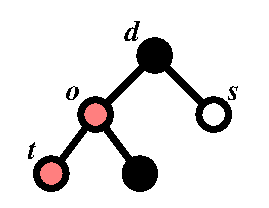
\includegraphics{pics/rbt-i}
\caption{Obecn� situace p�i INSERTu}
\label{rbt-i}
\end{figure}

Nejprve z�le�� na tom, jakou barvu m� $s$, str�c $t$:
\begin{enumerate}
\item $s$ je �erven�. Pak pouze p�ebarv�me $o$, $d$ a $s$ podle
obr�zku \ref{rbt-i1}.
Podm�nky 1 a 3 jsou spln�ny. Nyn� $d$ m��e b�t porucha, ov�em posunut� o 2
hladiny v��e. Vznikl 2t��s $(T,d)$.

\begin{figure}[!htb]
\centering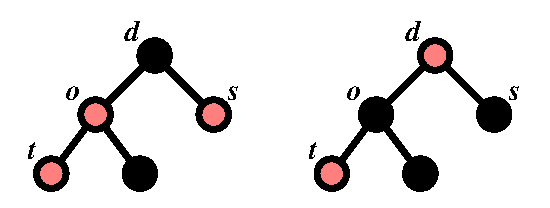
\includegraphics{pics/rbt-i1}
\caption{Oprava INSERTu p�ebarven�m}
\label{rbt-i1}
\end{figure}

\item $s$ je �ern�. Z�le�� na tom, zda hodnota $t$ le�� mezi hodnotami
$o$ a $d$ nebo ne. Jin�mi slovy, zda cesta $t$-$o$-$d$ obsahuje
\emph{zat��ku}.
\begin{enumerate}
\item Bez zat��ky:
Provedeme rotaci a p�ebarv�me podle obr�zku \ref{rbt-i2a}.
Spln�ny budou podm�nky 1, 2 i 3, tedy m�me �erveno�ern� strom.

\begin{figure}[!htb]
\centering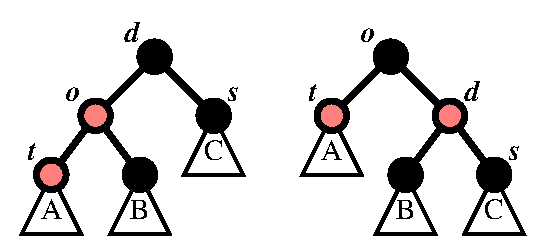
\includegraphics{pics/rbt-i2a}
\caption{Oprava INSERTu rotac� a p�ebarven�m}
\label{rbt-i2a}
\end{figure}

\item Se zat��kou:
Provedeme dvojitou rotaci a p�ebarv�me podle obr�zku \ref{rbt-i2b}.
Spln�ny budou podm�nky 1, 2 i 3, op�t m�me rovnou �erveno�ern� strom.

\begin{figure}[!htb]
\centering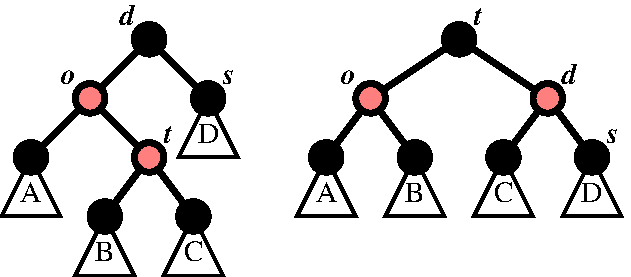
\includegraphics{pics/rbt-i2b}
\caption{Oprava INSERTu dvojitou rotac� a p�ebarven�m}
\label{rbt-i2b}
\end{figure}

\end{enumerate}
\end{enumerate}

\subsection{Operace DELETE}
Zat�mco INSERT se p��li� neli�il od sv� obdoby u AVL strom�, operace
DELETE u �erveno�ern�ch strom� je oproti AVL strom�m slo�it�j��
ment�ln�, ov�em jednodu��� �asov�.

Situace: odstra�ujeme vrchol $t$ (kter� nemus� reprezentovat
odstra�ovan� prvek --- viz DELETE v obecn�ch bin�rn�ch vyhled�vac�ch
stromech) a jeho syna, kter� je list.

Druh�ho syna $t$, $u$, d�me na m�sto smazan�ho $t$ a za�ern�me ho. T�m
m�me spln�n� podm�nky 1 a 2. Pokud byl ale $t$ �ern�, chyb� n�m na
cest�ch proch�zej�c�ch nyn� vrcholem $u$ jeden �ern� vrchol.
\begin{defn}
Strom a jeho vrchol $(T,u)$ nazveme \emph{3-t�m�� �erveno�ern� strom
(3t��s),} jestli�e plat�
\begin{itemize}
\item{1} Listy jsou �ern�. {\it (nezm�n�no)}
\item{2} Pokud m� �erven� vrchol otce, je otec �ern�. {\it (nezm�n�no)}
\item{3'}
V�echny cesty z ko�ene do listu neproch�zej�c� $u$ maj� stejn� po�et
�ern�ch vrchol�, nech� je to $k$. 
V�echny cesty z ko�ene do listu   proch�zej�c� $u$ maj� stejn� po�et
�ern�ch vrchol�, nech� je to $\ell$. 
A plat� $k-1 \leq \ell \leq k$.
\end{itemize}
Kdy� $u$ nen� ko�en a $\ell < k$, pak �ekneme, �e $u$ je \emph{porucha}.
\end{defn}

\begin{pozn}
Takov�mu vrcholu v 3t��s se n�kdy ��k� \emph{3-porucha}.
\end{pozn}

Nech� vrchol $u$  je porucha. Pak m��eme p�edpokl�dat, �e je 
obarven �ern�, jinak bychom ho p�ebarvili na �erno a t�m by se porucha 
odstranila a vznikl �erveno�ern� strom.

Situace: m�me 3t��s $(T,u)$, $u$ je porucha s otcem $o$, bratrem $b$ a
synovci $s1$, $s2$, viz obr�zek \ref{rbt-d}.

\begin{figure}[!htb]
\centering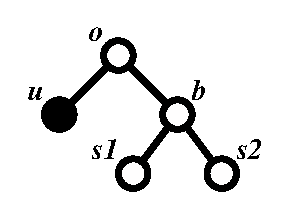
\includegraphics{pics/rbt-d}
\caption{Obecn� situace p�i DELETE}
\label{rbt-d}
\end{figure}
Oprava z�le�� na barv� vrcholu $b$:

\begin{enumerate}
\item Bratr je �ern�. 
Rozli�ujeme d�le 4 p��pady, z nich� jeden propaguje poruchu o hladinu
v�� a ostatn� skon�� s �erveno�ern�m stromem.

\begin{enumerate}
\item Otec i synovci jsou �ern�.
P�ebarv�me $b$ na �erveno, viz obr�zek \ref{rbt-d1a}. Dost�v�me 3t��s $(T,o)$,
tedy porucha je o hladinu v��e.

\begin{figure}[!htb]
\centering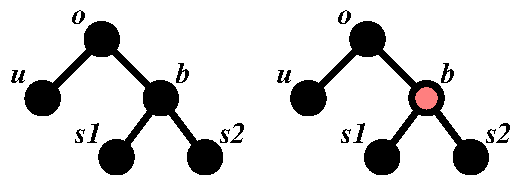
\includegraphics{pics/rbt-d1a}
\caption{��ste�n� oprava DELETE p�ebarven�m}
\label{rbt-d1a}
\end{figure}
\item \label{rbt-cd1b} Otec je �erven�, synovci �ern�.
P�ebarv�me otce a bratra podle obr�zku \ref{rbt-d1b} a dost�v�me
�erveno�ern� strom.

\begin{figure}[!htb]
\centering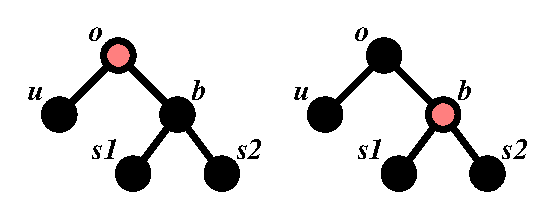
\includegraphics{pics/rbt-d1b}
\caption{Oprava DELETE p�ebarven�m}
\label{rbt-d1b}
\end{figure}
\item \label{rbt-cd1c} Synovec $s1$, jeho� hodnota le�� mezi hodnotami
otce a bratra, je �ern�, druh� synovec je �erven�.
P�ebarv�me a zrotujeme podle obr�zku \ref{rbt-d1c}, barva otce se
nem�n� (tj., vrchol $b$ bude m�t barvu, kterou p�vodn� m�l vrchol $o$).
Dost�v�me �erveno�ern� strom.

\begin{figure}[!htb]
\centering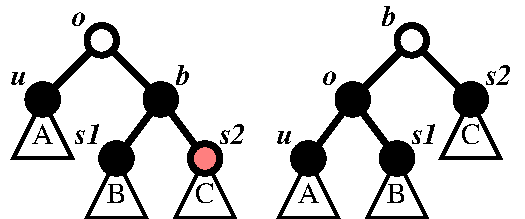
\includegraphics{pics/rbt-d1c}
\caption{Oprava DELETE p�ebarven�m a rotac�}
\label{rbt-d1c}
\end{figure}
\item \label{rbt-cd1d} Synovec $s1$, jeho� hodnota le�� mezi hodnotami
otce a bratra, je �erven�, druh� synovec m� libovolnou barvu.
P�ebarv�me a dvojit� zrotujeme podle obr�zku \ref{rbt-d1d} (tj., vrchol $s1$ 
bude m�t barvu, kterou p�vodn� m�l vrchol $o$ a barva vrcholu $s2$ se nezm�n�).
Dost�v�me �erveno�ern� strom.

\begin{figure}[!htb]
\centering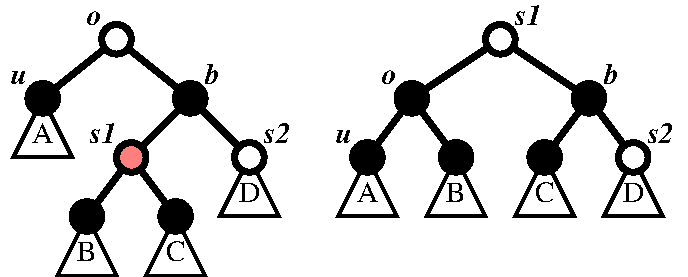
\includegraphics{pics/rbt-d1d}
\caption{Oprava DELETE p�ebarven�m a dvojitou rotac�}
\label{rbt-d1d}
\end{figure}

\end{enumerate}

\item Bratr je �erven�. Provedeme rotaci. 
Dostaneme strom ve tvaru, kter� je na \ref{rbt-d2}.
a aplikujeme p�edchoz� p��pad �.1. \\
P�esto�e to tak na prvn� pohled nevypad�, m�me vyhr�no, proto�e bratr 
poruchy je �ern� a otec �erven�, tedy p���t� oprava bude p��pad \ref{rbt-cd1b}, \ref{rbt-cd1c}, nebo \ref{rbt-cd1d} a skon��me s �erveno�ern�m 
stromem.

\begin{figure}[!htb]
\centering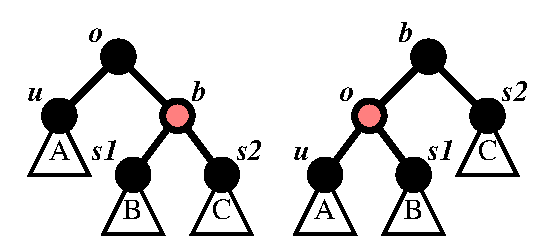
\includegraphics{pics/rbt-d2}
\caption{��ste�n� oprava DELETE p�ebarven�m a rotac�}
\label{rbt-d2}
\end{figure}

\end{enumerate}

\subsection{Z�v�ry}
Pro bin�rn� vyhled�vac� �erveno�ern� stromy lze implementovat MEMBER,
INSERT a DELETE tak, �e vy�aduj� �as $O(\log n)$ a INSERT pou��v�
nejv��e jednu (dvojitou) rotaci a DELETE pou��v� nejv��e dv� rotace
nebo rotaci a dvojitou rotaci. 

Jsou lep�� ne� AVL stromy, kter� p�i DELETE spot�ebuj� a� $\log n$
rotac�. Oproti v�hov� vyv�en�m strom�m i proti AVL strom�m jsou 
�erveno�ern� stromy jen
konstantn� lep��, ale i to je dobr�. P�i pou�it� bin�rn�ch vyhled�vac�ch 
strom� ve v�po�etn� geometrii nese informaci i rozlo�en� prvk� ve strom�, 
a tato informace se mus� po proveden� rotace nebo dvojit� rotace aktualizovat. 
To znamen� prohled�n� cel�ho stromu a tedy �as $O(n)$ za ka�dou rotaci a 
dvojitou rotaci nav�c. Pro tyto probl�my jsou �erveno�ern� stromy obzvl�t� 
vhodn�, proto�e minimalizuj� po�et pou�it�ch rotac� a dvojit�ch rotac�. 

�erveno�ern� stromy se pou��vaj� p�i implementaci $(2,4)$-strom�, se
kter�mi se sezn�m�me v dal�� kapitole. Vrchol 
se dv�ma syny je nahrazen jedn�m �ern�m vrcholem, vrchol se t�emi syny 
je nahrazen �ern�m vrcholem s jedn�m �erven�m synem a vrchol se �ty�mi 
syny je nahrazen �ern�m vrcholem se dv�ma syny. Pozor! Aktualiza�n� 
operace pro $(2,4)$-stromy neodpov�daj� aktualiza�n�m operac�m na 
�erveno�ern�ch stromech (i reprezentace prvk� je odli�n�).

�erveno�ern� stromy se pou��vaj� nap��klad ve 
\href{http://www.sgi.com/tech/stl/}%
{standardn� �ablonov� knihovn� jazyka C++ od SGI}, 
kter� je zahrnuta do GCC. M�te-li Linux, zkuste se pod�vat do
\path{/usr/include/g++-2/stl\_tree.h}; pokud pou��v�te OpenBSD, najdete
implementaci jak �erveno�ern�ch, tak splay strom� v
\path{/usr/include/sys/tree.h}.
\footnote{A pokud v�te o podobn� dostupn�ch implementac�ch jin�ch
datov�ch struktur z t�hle p�edn�ky, sem s nimi!}

% ==========================================================================
% Sou��st skript Datov� struktury. ds.tex
% Authors: Martin Vidner
%	   Vladimir Kotal
\markright{$ $Id$ $}

\chapter{$(a,b)$ stromy}

% --------------------------------------------------------------------------
\section{Z�kladn� varianta}

Nech� $a, b \in \mathbb{N}, a \leq b$. Strom je $(a,b)$ strom, kdy�
plat�
\begin{enumerate}
\item Ka�d� vnit�n� vrchol krom� ko�ene m� alespo� $a$ a nejv��e $b$
syn�.
\item Ko�en m� nejv��e $b$ syn�. Pokud $a \geq 2$, pak m� alespo� 2
syny, nebo je listem.
\item V�echny cesty z ko�ene do listu jsou stejn� dlouh�.
\end{enumerate}
\exercise
{Co by se stalo, kdybychom definici zjednodu�ili a m�sto podm�nek 1 a
2 po�adovali, aby \emph{ka�d�} vrchol m�l $a$ a� $b$ syn�?}{Nebyly by
mo�n� mal� $(a,b)$ stromy.}

\begin{figure}%[!htb]
\centering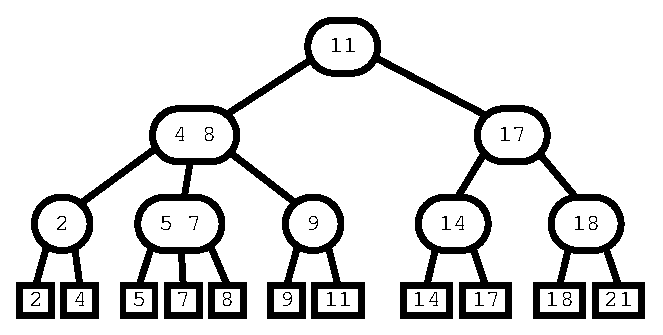
\includegraphics{pics/abt}
\caption{P��klad $(a,b)$ stromu}
\label{abt}
\end{figure}

\begin{defn}
Jsou-li synov� ka�d�ho vrcholu o��slov�ni, m��eme
definovat \emph{lexikografick� uspo��d�n� vrchol� na stejn� hladin�}.

$u \leq_l v$, jestli�e $\text{otec } u <_l \text{otec } v$ nebo
$\text{otec } u = \text{otec } v$, $u$ je $i$-t� syn, $v$ je $j$-t� syn
a $i \leq j$.
\end{defn}

\begin{pozn}
Prvky z mno�iny $S$ koresponduj� s listy $T$ tak, �e $s < s', s,s' \in S$,
pr�v� kdy� list odpov�daj�c� $s <_l$ list odpov�daj�c� $s'$.
\end{pozn}

Pozorov�n�: Bu� $T$ $(a,b)$ strom s hloubkou $h$. Plat�
\[
2 a^{h-1} \leq \text{po�et list� $T$} \leq  b^h,
\]
tedy pro libovoln� $n$ m� ka�d� $(a,b)$ strom $T$ s $n$ listy 
hloubku $\Theta(\log n)$.

% ..........................................................................
\subsection{Reprezentace mno�iny $S$ $(a,b)$ stromem}

M�jme $S \subseteq U$, p�i�em� universum je line�rn� uspo��dan�.
$(a,b)$ strom $T$ reprezentuje mno�inu $S$, jestli�e existuje
jednozna�n� p�i�azen� prvk� $S$ list�m $T$, kter� zachov�v� uspo��d�n�.

Pot�ebujeme nav�c podm�nku
\begin{enumerate}
\item[4.] $a \geq 2$ a $b \geq 2a - 1$ 
\end{enumerate}

Struktura vnit�n�ho vrcholu $v$:
\begin{itemize}
\item $\rho_v$ je po�et syn�
\item $S_v[1\ .. \ \rho_v]$ je pole ukazatel� na syny
\item $H_v[1\ .. \ \rho_v - 1]$: $H_v[i]$ je maxim�ln� prvek 
v~podstromu $S_v[i]$ 
\end{itemize}

% ..........................................................................
\subsection{MEMBER($x$) v $(a,b)$ stromu}
\begin{algorithmic}
\STATE \COMMENT{vyhled�n� $x$}
\STATE $t := \text{ko�en}$
\WHILE {$t$ nen� list}
	\STATE $i := 1$
	\WHILE {$H_t[i] < x \land i < \rho_t$}
		\STATE $i := i + 1$
	\ENDWHILE
	\STATE $t := S_t[i]$ 
\ENDWHILE
\STATE \COMMENT{testov�n� $x$}
\IF {$t$ reprezentuje $x$}
	\STATE $x \in S$
\ELSE
	\STATE $x \notin S$
\ENDIF
\end{algorithmic}

% ..........................................................................
\subsection{INSERT($x$) do $(a,b)$ stromu}
\begin{algorithmic}
\STATE vyhled�n� $x$
\IF {$t$ nereprezentuje $x$}
	\STATE $o := \text{otec } t$
	\STATE vrcholu $o$ p�idej nov�ho syna $t'$ 
	reprezentuj�c�ho $x$
	\STATE za�a� $t'$ na spr�vn� m�sto mezi jeho bratry
	a uprav $\rho_o$, $S_o$ a $H_o$
	\STATE $t := o$
	\WHILE {$\rho_t > b$}
		\STATE \COMMENT {�t�pen� 
				--- m��eme prov�st d�ky podm�nce 4}
		\STATE rozd�l $t$ na $t_1$ a $t_2$ 
		\STATE \quad k $t_1$ dej prvn�ch 
			$\lfloor (b+1)/2 \rfloor$ syn� $t$
		\STATE \quad k $t_2$ dej zbyl�ch 
			$\lceil (b+1)/2 \rceil$ syn� $t$
		\STATE $o := \text{otec } t$
		\STATE uprav $\rho_o$, $S_o$ a $H_o$
		\STATE \COMMENT {p�i �t�pen� ko�ene je�t� mus�me
				vytvo�it nov� ko�en}
		\STATE $t := o$
	\ENDWHILE
\ENDIF
\end{algorithmic}

% ..........................................................................
\subsection{DELETE($x$) z $(a,b)$ stromu}
\begin{algorithmic}
\STATE vyhled�n� $x$, nav�c si zapamatuj vrchol $u$, 
	v jeho� poli $H_u$ je $x$
\IF {$t$ reprezentuje $x$}
	\STATE $o := \text{otec } t$
	\STATE odstra� $t$
	\STATE uprav $H_o$, $H_u$ \COMMENT {...}
	\STATE uprav $S_o$ a $\rho_o$
	\STATE $t := o$
	\WHILE {$\rho_t < a \land t \text{ nen� ko�en}$}
		\STATE $v := \text{bezprost�edn� bratr } t$ 
		\IF[sm�me spojit] {$\rho_v = a$}
			\STATE \COMMENT {Spojen�}
			\STATE $o := \text{otec } t$
			\STATE slu� $v$ a $t$ do $t$
			\STATE uprav $\rho_o$, $S_o$ a $H_o$
			\STATE $t := o$
		\ELSE[$\rho_v > a$, spojen� by mohlo m�t v�ce ne� $b$ syn�]
			\STATE \COMMENT {P�esun}
			\STATE p�esu� krajn�ho syna $v$ do $t$
			\STATE uprav $H_{\text{otec } t}$
		\ENDIF
	\ENDWHILE
	\IF {$t$ je ko�en a m� jen jednoho syna}
		\STATE sma� $t$
	\ENDIF
\ENDIF
\end{algorithmic}

% ..........................................................................
\subsection{Shrnut�}
Operace �t�pen�, p�esun i spojen� vy�aduj� konstantn� �as. 
\begin{theorem}
Operace MEMBER, INSERT a DELETE pro $(a,b)$ stromy vy�aduj� �as
$O(\log n)$, kde $n$ je velikost reprezentovan� mno�iny.
\end{theorem}

S $H$ a $S$ jsme pracovali jako se seznamy, nepot�ebujeme, aby to byla
pole. T�m se zjednodu�� implementace. 
\mnote{V�hodnost pro vn�j�� pam�ti?}

% ..........................................................................
\subsection{Jak volit parametry $(a,b)$}

Pro vnit�n� pam� je vhodn� $a = 2$ nebo $a=3$, $b = 2a$.
Pro vn�j�� pam� je vhodn� $a \approx 100$, $b = 2a$.

Pro minimalizaci pam�ov�ch n�rok� je v�hodn� $b = 2a-1$,
pro minimalizaci �asov�ch n�rok� je v�hodn� $b = 2a$.
\mnote{pro�? pr� se k tomu je�t� dostaneme}

% --------------------------------------------------------------------------
\section{Dal�� operace}

%MIN, MAX

% ..........................................................................
Pro operaci JOIN je vhodn� spolu se stromem uchov�vat tak� 
nejv�t�� prvek reprezentovan� mno�iny.

\subsection{Algoritmus JOIN($T_1, T_2$) pro $(a,b)$ stromy}
\begin{algorithmic}
\REQUIRE {$T_1$ reprezentuje $S_1$, $T_2$ reprezentuje $S_2$ 
	a $\max S_1 < \min S_2$ }
\STATE $n := \text{hloubka } T_1 - \text{hloubka } T_2$ 
\IF {$n \geq 0$}
	\STATE $t := \text{ko�en } T_1$
	\WHILE {$n > 0$}
		\STATE $t := \text{posledn� syn } t$
		\STATE $n := n - 1$
	\ENDWHILE
	\STATE Spoj $t$ s ko�enem $T_2$ a vytvo� nov� vrchol $t'$.
	\COMMENT {zde se vyu�ije znalost nejv�t��ho prvku mno�iny $S_1$}
	\WHILE {$\rho_t > b$}
		\STATE �t�pen� $t$		
		\STATE $t := \text{otec } t$
	\ENDWHILE
\ELSE
	\STATE \COMMENT {analogicky: ko�en $T_2$, prvn� syn \dots}
\ENDIF
\end{algorithmic}

JOIN vy�aduje �as $O(\text{rozd�l hloubek strom�}) 
\leq O(\log(|S_1| + |S_2|))$.

% ..........................................................................
\subsection{Algoritmus SPLIT($x, T$) pro $(a,b)$ strom}
\begin{algorithmic}
\ENSURE {Vytvo�� 
	$T_1$ reprezentuj�c� $\{ s \in S: s < x \}$ a
	$T_2$ reprezentuj�c� $\{ s \in S: s > x \}$}
\STATE Nech� $Z_1$ a $Z_2$ jsou pr�zdn� z�sobn�ky
\STATE $t := \text{ko�en } T$
\WHILE {$t$ nen� list}
	\STATE $i := 1$
	\WHILE {$H_t[i] < x \land i < \rho_t$}
		\STATE $i := i + 1$ 
	\ENDWHILE
	\STATE Vytvo� strom $T_1$, jeho� ko�en %$t_1$
	m� syny $S_t[1] \dots S_t[i-1]$
	\STATE Vytvo� strom $T_2$, jeho� ko�en %$t_2$
	m� syny $S_t[i+1] \dots S_t[\rho_t]$
	\IF {$T_1$ nen� jednoprvkov� strom}
		\STATE Push($Z_1, T_1$)
	\ENDIF
        \IF {$T_2$ nen� jednoprvkov� strom}
		\STATE Push($Z_2, T_2$)
	\ENDIF
	\STATE $t := S_t[i]$ 
\ENDWHILE
\IF {$t$ reprezentuje prvek r�zn� od $x$}
	\STATE Ud�lej z $t$ $(a,b)$ strom a vlo� ho
	do p��slu�n�ho z�sobn�ku.
\ENDIF
\STATE $T_1 := \text{STACKJOIN}(Z_1)$ \COMMENT {viz d�le}
\STATE $T_2 := \text{STACKJOIN}(Z_2)$
\end{algorithmic}

�as roz�ez�v�n� stromu je �m�rn� jeho hloubce. Celkov� �as operace
SPLIT ov�em z�vis� je�t� na slo�itosti operace STACKJOIN.

% ..........................................................................
\subsection{Algoritmus STACKJOIN($Z$) pro z�sobn�k $(a,b)$ strom�}
\begin{algorithmic}
\STATE $T := \text{Pop}(Z)$
\WHILE {$Z \ne \emptyset$}
	\STATE $T' := \text{Pop}(Z)$
	\STATE $T := \text{JOIN}(T, T')$
\ENDWHILE
\end{algorithmic}

Nech� $Z$ obsahuje $(a,b)$ stromy $T_1 \dots T_k$, p�i�em� $T_1$ je
vrchol z�sobn�ku.
Plat�
\[
\forall i:\ \text{hloubka }T_i \leq \text{hloubka }T_{i+1}
\]
\begin{align*}
\text{�as STACKJOIN}
 & = \text{hloubka }T_2 - \text{hloubka }T_1 + 1 \\
 & + \text{hloubka }T_3 - \text{hloubka }T_2 + 1 \\
 & + \dots \\
 & + \text{hloubka }T_k - \text{hloubka }T_{k-1} + 1 \\
 & = \text{hloubka }T_k - \text{hloubka }T_1 + \text{po�et JOIN�} \\
 & = O(\text{hloubka }T) = O(\log |S|)
\end{align*}

Tedy i operace SPLIT vy�aduje �as $O(\log |S|)$.

% ..........................................................................
\subsection{Algoritmus FIND($T, k$) pro $(a,b)$ strom}
Nalezen� $k$-t�ho nejmen��ho prvku.

Roz����me reprezentaci stromu a ka�d�mu vnit�n�mu vrcholu $v$ p�id�me:
\begin{itemize}
\item $K_v[1\ .. \ \rho_v]$: $K_v[i]$ je po�et list�
v~podstromu $S_v[i]$ 
\end{itemize}

\begin{algorithmic}
\STATE $t := \text{ko�en }T$
\WHILE {$t$ nen� list}
	\STATE $i := 1$
	\WHILE {$K_t[i] < k \land i < \rho_t$}
		\STATE $k := k - K_t[i]$ 
		\STATE $i := i + 1$ 
	\ENDWHILE
	\STATE $t := S_t[i]$ 
\ENDWHILE
\IF {$k > 1$}
	\STATE \textbf{return} nil \COMMENT {$k > |S|$}
\ELSE
	\STATE \textbf{return} $t$
\ENDIF
\end{algorithmic}

�asov� slo�itost je op�t logaritmick�, p�i�em� d��ve uveden� operace
nejsou zpomaleny t�m, �e aktualizuj� pole (seznam) $K$.

% ..........................................................................
\subsection{A-sort}

Na prvn� pohled se zd�, �e pou�it� $(a,b)$ strom� ke t��d�n� nen�
v�hodn�. Pam�ov� n�roky budou oproti b�n�mu t��d�n� v poli asi
p�tkr�t v�t��. Aby se tedy t��d�n� $(a,b)$ stromem vyplatilo, muselo
by p�in�st zv��en� rychlosti. V t�to ��sti p�edvedeme, �e to skute�n�
je mo�n�, jestli�e vstupn� data jsou ji� ��ste�n� set��d�n�.

Pro ��ely A-sortu roz����me reprezentaci takto:
\begin{itemize}
\item Listy stromu jsou propojeny do seznamu
\item Je zn�ma cesta z nejmen��ho (nejlev�j��ho) listu do ko�ene
(ulo�en� nap�. v z�sobn�ku)
\end{itemize}

Pou�ijeme $(2,3)$-strom.\mnote{pro�?}

Nech� vstupn� posloupnost je $a_1, \dots, a_n$. Postupn� odzadu
vkl�d�me jej� prvky do stromu modifikovan�m INSERTem:
\begin{algorithmic}
\STATE $k := n$
\WHILE {$k > 1$}
	\STATE A-INSERT($a_k$)
	\STATE $k := k - 1$
\ENDWHILE
\end{algorithmic}
Na konci p�e�teme set��d�nou posloupnost pomoc� spojov�ho seznamu
list�.

A-INSERT, stejn� jako p�vodn� INSERT, najde spr�vn� list a potom
p��padn� p�id� nov� prvek. K nalezen� spr�vn�ho listu ov�em vyu��v�
cestu z nejmen��ho listu. Zde uveden� verze A-INSERTu odstra�uje 
duplicitn� prvky, operaci lze pochopiteln� upravit tak, �e nech�v� 
duplicitn� prvky, kter� z�st�vaj� ve stejn�m po�ad�.
\begin{algorithmic}
\STATE \COMMENT {Nalezen�}
\STATE $t := \text{nejmen�� list}$
\REPEAT
	\STATE $t := \text{otec } t$
\UNTIL {$t \text{ je ko�en} \lor x \leq H_t[1]$}
\STATE \COMMENT {nyn� jako v p�vodn�m INSERTu, pouze jsme jinak
inicializovali $t$}
\WHILE {$t$ nen� list}
	\STATE $i := 1$
	\WHILE {$H_t[i] < x \land i < \rho_t$}
		\STATE $i := i + 1$
	\ENDWHILE
	\STATE $t := S_t[i]$ 
\ENDWHILE
\STATE \COMMENT {P�id�n�}
\IF {$t$ nereprezentuje $x$}
	\STATE $o := \text{otec } t$
	\STATE vrcholu $o$ p�idej nov�ho syna $t'$ 
	reprezentuj�c�ho $x$
	\STATE za�a� $t'$ na spr�vn� m�sto mezi jeho bratry
	a uprav $\rho_o$, $S_o$ a $H_o$
	\STATE $t := o$
	\WHILE {$\rho_t > b$}
		\STATE \COMMENT {�t�pen� 
				--- m��eme prov�st d�ky podm�nce 4}
		\STATE rozd�l $t$ na $t_1$ a $t_2$ 
		\STATE \quad k $t_1$ dej prvn�ch 
			$\lfloor (b+1)/2 \rfloor$ syn� $t$
		\STATE \quad k $t_2$ dej zbyl�ch 
			$\lceil (b+1)/2 \rceil$ syn� $t$
		\STATE $o := \text{otec } t$
		\STATE uprav $\rho_o$, $S_o$ a $H_o$
		\STATE \COMMENT {p�i �t�pen� ko�ene je�t� mus�me
				vytvo�it nov� ko�en}
	\ENDWHILE
\ENDIF
\end{algorithmic}

�as A-sortu
= $\sum$ �asu vyhled�n� + $\sum$ �asu p�id�n� + �as vytvo�en� v�stupn�
posloupnosti.
�as vytvo�en� v�stupn� posloupnosti = $O(n)$.

$\sum \text{�asu p�id�n�} 
= \text{po�et p�idan�ch vrchol�} \cdot \text{�as p�id�n� vrcholu}
+ \text{po�et �t�pen�} \cdot \text{�as �t�pen�}
= O(n) \cdot O(1)
+ \text{po�et �t�pen�} \cdot O(1).$ 
Proto�e se zde neprov�d� operace DELETE, lze ka�d�mu �t�pen� p�i�adit 
vnit�n� vrchol, kter� byl p�i tomto �t�pen� vytvo�en (�t�pen� rozd�l� 
vrchol $t$ na dva vrcholy $t_1$ a $t_2$, budeme p�edpokl�dat, �e 
vrchol $t_1$ je pokra�ov�n�m vrcholu $t$ a vrchol $t_2$ je vrchol 
vznikl� p�i �t�pen�). Tedy po�et �t�pen� je men�� ne� po�et vnit�n�ch 
vrchol� (p�i �t�pen� ko�ene vznik� nav�c je�t� nov� ko�en),  
tedy $\sum \text{�asu p�id�n�} = O(n).$

�as A-sortu tedy z�vis� hlavn� na celkov�m �ase vyhled�n� prvk�.
Ozna�me
\[
f_i = |\{ j > i:\ a_j < a_i \}|,
\]
tedy po�et prvk� posloupnosti, kter� v neset��d�n� posloupnosti
n�sleduj� $a_i$, ale v set��d�n� pat�� p�ed $a_i$. P�i vyhled�n� $a_i$
ve stromu vyjad�uje $f_i$ po�et list� nalevo od $a_i$. �as
vyhled�n� $a_i$ je tedy $O(\log f_i)$ a celkov� �as vyhled�n� je 
$O(\sum \log f_i)$.
\mnote{o�et�it $\log 0$}

Hodnota $F = \sum f_i$, zvan� 
\emph{po�et inverz�}, \mnote{nebo transpozic? standardn� term�n?}%
vyjad�uje uspo��danost vstupn�
posloupnosti. Pro spr�vn� uspo��danou posloupnost je $F = 0$, pro
obr�cen� uspo��danou posloupnost je $F = n (n-1) / 2$. To jsou tak�
mezn� hodnoty, jich� m��e $F$ nab�vat.

Z vlastnost� logaritmu a srovn�n�m geometrick�ho a aritmetick�ho
pr�m�ru dost�v�me
\[
\sum \log f_i = \log \prod f_i = n \log \sqrt[n]{\prod f_i}
\leq n \log (F/n).
\]

A-sort tedy vy�aduje �as $O(n \max(1, \log((F+1)/n)))$. V nejhor��m
p��pad� to je $O(n \log n)$ a Mehlhorn a Tsakalidis uk�zali, �e A-sort
je lep�� ne� Quicksort v p��pad�, �e $F \leq 0.02 n^{1.57}$.
Naproti tomu Insertsort, jednoduch� algoritmus, kter� postupn�
line�rn�m prohled�n�m zat�i�uje prvky pole do jeho ji� set��d�n�ho
po��te�n�ho �seku, vy�aduje �as $O(n + F)$, co� je v nejhor��m p��pad�
$O(n^2)$.

Zb�v� je�t� zd�vodnit, pro� pou��t $(2,3)$-stromy. V�me, �e $(2,3)$-stromy 
maj� nejmen�� prostorov� n�roky mezi $(a,b)$-stromy. Na druh� stran� v�ak 
$(2,3)$-stromy v obecn�m p��pad� vy�aduj� zbyte�n� mnoho vyva�ovac�ch 
operac�, a proto jsou v�razn� pomalej�� ne� nap�. $(2,4)$-stromy. Proto�e 
v�ak A-sort nepou��v� operaci DELETE, uk�zali jsme (viz po�et operac� 
�t�pen�), �e pro A-sort to nen� pravda. Zde $(2,3)$-stromy pat�� mezi 
nejrychleji pracuj�c� $(a,b)$-stromy.

% --------------------------------------------------------------------------
\section{Paraleln� p��stup do $(a,b)$ strom�}

P�i operac�ch INSERT a DELETE jsme nejprve sestupovali stromem dol� a�
k list�m, potom jsme se vraceli nahoru a �t�pili nebo spojovali
vrcholy. To znemo��uje dovolit paraleln� p��stup do stromu. Procesu,
kter� je ve f�zi vyhled�n�, by se mohlo st�t, �e mu jin� proces zm�n�
strom ``pod rukama''. St�vaj�c� operace INSERT a DELETE tedy po�aduj�
v�lu�n� p��stup ke stromu.

Nyn� p�edvedeme paraleln� verzi t�chto operac�, kde se �t�pen� nebo
spojov�n� prov�d� ji� p�i sestupu. Potom ji� nen� nutn� se vracet a je
tedy mo�n� rovnou odemykat ��sti stromu, ke kter�m ji� dan� proces
nebude p�istupovat. Cenou za tento p��stup jsou zbyte�n�
�t�pen�/spojen�.
\mnote{ud�lat obr�zek ilustruj�c� zbyte�n� �/s}

Pot�ebujeme omezit $b$: podm�nku $b \geq 2a - 1$ zp��sn�me na
\begin{enumerate}
\item[4'.] $a \geq 2$ a $b \geq 2a$ 
\end{enumerate}

% ..........................................................................
\subsection{Paraleln� INSERT($x$) do $(a,b)$ stromu}
\begin{algorithmic}
\STATE $o := \text{lock}(\text{nadko�en})$ \COMMENT {Nadko�en
je implementa�n� pom�cka. Slou�� k zamknut�
p��stupu k cel�mu stromu a uchov�v� $\max(S)$}
\STATE $t := \text{ko�en}$ 
\STATE \COMMENT {Invariant mezi pr�chody cyklem:
	$o$ je otec $t$, $o$ je jedin� vrchol zamknut� t�mto procesem.}
\WHILE {$t$ nen� list}
	\STATE $i := 1$
	\WHILE {$i < \rho_t \land H_t[i] < x$}
		\STATE $i := i + 1$
	\ENDWHILE
	\STATE $s := S_t[i]$ 
	\STATE \COMMENT {preventivn� roz�t�pen�:}
	\IF {$\rho(t) = b$}
		\STATE rozd�l $t$ na $t_1$ a $t_2$: \COMMENT {viz 4'}
		\STATE \quad k $t_1$ dej prvn�ch 
			$\lfloor (b+1)/2 \rfloor$ syn� $t$
		\STATE \quad k $t_2$ dej zbyl�ch 
			$\lceil (b+1)/2 \rceil$ syn� $t$
		\STATE \quad $t_1$ p�edch�z� $t_2$
		\STATE uprav $\rho_o$, $S_o$ a $H_o$
		\STATE \COMMENT {implic.: uprav $\rho_{t_1}$, \dots, $H_{t_2}$}
		\STATE \COMMENT {p�i �t�pen� ko�ene je�t� mus�me
				vytvo�it nov� ko�en}
		\STATE $n := t_j$, kde $s$ je syn $t_j$
	\ELSE
		\STATE $n := t$
	\ENDIF
	\STATE lock($n$) 
	\STATE unlock($o$) 
	\STATE $o := n$
	\STATE $t := s$
\ENDWHILE
\IF {$t$ nereprezentuje $x$}
	\STATE vrcholu $o$ p�idej nov�ho syna $t'$ 
	reprezentuj�c�ho $x$
	\STATE za�a� $t'$ na spr�vn� m�sto mezi jeho bratry
	a uprav $\rho_o$, $S_o$ a $H_o$
\ENDIF
\STATE unlock($o$)
\end{algorithmic}

% ..........................................................................
\subsection{Paraleln� DELETE($x$) z $(a,b)$ stromu}
\begin{algorithmic}
\STATE $o := \text{lock}(\text{nadko�en})$ \COMMENT {Nadko�en
je implementa�n� pom�cka. Slou�� k zamknut�
p��stupu k cel�mu stromu a uchov�v� $\max(S)$}
\STATE $t := \text{ko�en}$ 
\STATE $h := \textbf{nil}$ \COMMENT 
	{Jakmile $h \neq \textbf{nil}$, 
	$x \in H_h$ a $h$ bude zam�en� do konce procesu.}
\STATE \COMMENT {Invariant mezi pr�chody cyklem:
	$o$ je otec $t$, $o$ je krom� $h$ jedin� vrchol
	zamknut� t�mto procesem.}
\WHILE {$t$ nen� list}
	\STATE $i := 1$
	\WHILE {$i < \rho_t \land H_t[i] < x$}
		\STATE $i := i + 1$
	\ENDWHILE
	\IF {$H_t[i] = x$}
		\STATE $h := t$
	\ENDIF
	\STATE $s := S_t[i]$ 
	\STATE \COMMENT {preventivn� spojen�/p�esun:}
	\IF {$\rho(t) = a$}
		\STATE $v := \text{bezprost�edn� bratr } t$ %bratr[fi]=_v_eli
		\IF[sm�me spojit] {$\rho_v = a$}
			\STATE \COMMENT {Spojen�}
			\STATE slu� $v$ a $t$ do $t$ \COMMENT {viz 4'}
			\STATE uprav $\rho_o$, $S_o$ a $H_o$
			\STATE $t := o$
		\ELSE[$\rho_v > a$, spojen� by m�lo v�ce ne� $b$ syn�]
			\STATE \COMMENT {P�esun}
			\STATE p�esu� krajn�ho syna $v$ do $t$
			\STATE uprav $H_o$, $H_v$ a $H_t$
		\ENDIF
	\ENDIF
	\STATE lock($t$) 
	\IF {$o \neq h$}
		\STATE unlock($o$)
	\ENDIF
	\STATE $o := t$
	\STATE $t := s$
\ENDWHILE
\IF {$t$ reprezentuje $x$}
	\STATE odstra� $t$
	\STATE uprav $H_o$, $H_h$
	\STATE uprav $S_o$ a $\rho_o$
	\STATE unlock($h$)
\ENDIF
\STATE unlock($o$)
\end{algorithmic}


% --------------------------------------------------------------------------
\section{Slo�itost posloupnosti operac� na $(a,b)$ stromu}

A-sort funguje jednak proto, �e v p�edt��d�n� posloupnosti rychle
najde m�sto, kam se m� vkl�dat, jednak proto, �e se p�i sam�ch
INSERTech ({\it a d�ky spr�vn�m $a$, $b$?}) prov�d� m�lo
vyva�ovac�ch krok�. V t�to sekci se pod�v�me na po�et vyva�ovac�ch
krok� pro posloupnost operac� INSERT a DELETE.

Nech� $b \geq 2a$.
\begin{theorem}
M�jme posloupnost $n$ operac� INSERT a DELETE aplikovanou na pr�zdn�
$(a,b)$ strom. Ozna�me $P$ po�et p�esun� p�i prov�d�n� posloupnosti,
$SP$ po�et spojen� a $ST$ po�et �t�pen�. D�le ozna�me $P_h$, $SP_h$ a
$ST_h$ po�et p�esun�. spojen� a �t�pen�, kter� nastanou ve v��ce $h$
(listy maj� v��ku 0).

Nech�
\begin{equation}
\begin{split}
% this is ``occult alignment'' :)
c = \min
 &\left(
   \phantom{b - \vphantom{x}}
        \min \left( 2a-1, \left\lceil \frac{b+1}{2}\right\rceil  \right) - a, 
  \right.\\
 &\left.
		\phantom{\left(
		\vphantom{\left. \frac xy\right.}
		\right.}
    b - \max \left( 2a-1, \left\lfloor\frac{b+1}{2}\right\rfloor \right)
   \phantom{\vphantom{x} - a}
  \right)
\end{split}
\end{equation}

Pak plat�
%\renewcommand{\labelenumi}{\alph{enumi}}
\begin{eqnarray}
P &\leq& n \\
\label{ab-v-stsp}
(2c-1)ST + cSP &\leq& n + c + \frac c{a+c-1} (n-2) \\
\label{ab-v-sthsph}
P_h + SP_h + ST_h &\leq& \frac{2 n^{c+2}}{(c+1)^h} 
\end{eqnarray}
\end{theorem}

Plat� $c \geq 1$ (p�i $b = 2a$ dokonce $c = 1$). Z toho
\begin{equation}
ST + SP \leq \frac nc + 1 + \frac{n-2}a,
\end{equation}
tedy line�rn� vzhledem k $n$.

Pro paraleln� verze INSERT a DELETE plat� obdobn� v�ta, kdy� 
$b \geq 2a + 2$.

Pro d�kaz pou�ijeme \emph{bankovn� paradigma}: datovou strukturu
ohodnot�me podle toho, jak je ``uklizen�''. Operace, kter� datovou
strukturu ``uklid�'', zv�t�� jej� ``z�statek na ��t�''. Ty, kter� ji
``naru��'', z�statek zmen��. Potom najdeme vztah mezi z�statkem a
spot�ebovan�m �asem.
{\it Tohle pokulh�v�. Myslel jsem si, �e z�statek je n�co jako �as v
konzerv�, kter� si pomal� operace berou od rychl�ch \dots, ale  v
tomhle p��pad� to asi funguje jinak.}
\mnote{vyjasnit}
\mnote{pou�iju $z$ jako z�statek m�sto $b$ jako balance, proto�e
souvislost s vyva�ov�n�m stromu je zde sp�� matouc�}

$(a,b)$ stromy jsou uklizen�, kdy� maj� vrcholy po�et syn� n�kde
uprost�ed mezi $a$ a $b$. Tehdy nenastane v brzk� dob� vyva�ovac�
operace. V tomto smyslu definujme:
\begin{align}
z(v) &=
	\min ( \rho_v - a, b - \rho_v, c ) 
	&&\text{$v$ je vnit�n� vrchol r�zn� od ko�ene}\\
z(\text{ko�en}) &=
        \min ( \rho_v - 2, b - \rho_v, c ) 
\end{align}

Pro strom $T$ definujme 
\[
z(T) = \sum_{v \in T} z(v)
\]
\[
z_h(T) = \sum_{\substack{v \in T\\v \text{ m� v��ku } h}} z(v)
\]
Plat�
\[
z(T) = \sum_h z_h(t)
\]

Podobn� jako u �erveno�ern�ch strom� definujme parci�ln� $(a,b)$-strom:
\begin{defn}
$(T,v)$ je \emph{parci�ln� $(a,b)$-strom,} kdy� $v$ je vnit�n� vrchol $T$
r�zn� od ko�ene a
krom� $v$ jsou spln�ny podm�nky pro $(a,b)$-strom a
$a-1 \leq \rho_v \leq b+1$.
\end{defn}

Z definice z�statku vypl�vaj� tyto vlastnosti:
\begin{align}
\label{ab-1}
  \rho_v = a-1 \text{ nebo }b+1 &\implies z(v) = -1\\
\label{ab-0}
  \rho_v = a \text{ nebo } b    &\implies z(v) = 0\\
\label{ab-spojeni}
  \rho_v = 2a-1                 &\implies z(v) = c\\
\label{ab-stepeni}
  \rho_u = \left\lfloor\frac{b+1}{2}\right\rfloor \land
  \rho_v = \left\lceil \frac{b+1}{2}\right\rceil
                                &\implies z(u)+z(v) \geq 2c - 1\\
\label{ab-presun}
  |\rho_u - \rho_v| \leq 1      &\implies z(u) \geq z(v) - 1
\end{align}

\subsection{p�id�n�/ubr�n� listu}
M�jme $(a,b)$-strom $T$ a p�id�me nebo ubereme list, jeho� otec je $v$.
Pak vznikne parci�ln� $(a,b)$-strom $(T',v)$ a plat�:
\begin{align}
  z_1(T')        & \geq z_1(T) - 1\\
  z_h(T')        & = z_h(T) \quad h>1\\
  z(T')          & \geq z(T) - 1
\end{align}

\subsection{�t�pen�}
M�jme parci�ln� $(a,b)$-strom $(T,v)$, kde $v$ je ve v��ce $h$.
Nech� $T'$ vznikl \emph{�t�pen�m $v$}. 
Pak $(T',\text{otec }v$ je parci�ln� $(a,b)$-strom a plat�:
\begin{align}
  z_h(T')       & \geq 2c + z_h(T)
	\qquad\text{z \ref{ab-1} a \ref{ab-stepeni}}\\
  z_{h+1}(T')   & \geq z_{h+1}(T) - 1\\
  z_i(T')       & = z_i(T) \quad i \neq h, h+1\\
  z(T')         & \geq z(T) + 2c - 1
\end{align}

\subsection{spojen�}
M�jme parci�ln� $(a,b)$-strom $(T,v)$, kde $\rho_v = a-1$ a 
$v$ je ve v��ce $h$, $y$ je bezprost�edn� bratr $v$.
Nech� $\rho_y = a$ a $T'$ vznikl \emph{spojen�m $v$ a $y$}. 
Pak $(T',\text{otec }v$ je parci�ln� $(a,b)$-strom a plat�:
\begin{align}
  z_h(T')       & \geq c + 1 + z_h(T)
	\qquad\text{z \ref{ab-1}, \ref{ab-0} a \ref{ab-spojeni}}\\
  z_{h+1}(T')   & \geq z_{h+1}(T) - 1\\
  z_i(T')       & = z_i(T) \quad i \neq h, h+1\\
  z(T')         & \geq z(T) + c
\end{align}

\subsection{p�esun}
M�jme parci�ln� $(a,b)$-strom $(T,v)$, kde $\rho_v = a-1$ a 
$v$ je ve v��ce $h$, $y$ je bezprost�edn� bratr $v$.
Nech� $\rho_y > a$ a $T'$ vznikl \emph{p�esunem syna od $y$ k $v$}. 
Pak $T'$ je $(a,b)$-strom a plat�:
\begin{align}
  z_h(T')       & \geq z_h(T)
	\qquad\text{z \ref{ab-1}, \ref{ab-0} a \ref{ab-presun}}\\
  z_i(T')       & = z_i(T) \quad i \neq h\\
  z(T')         & \geq z(T)
\end{align}

Nech� po skon�en� posloupnosti operac� m�me $(a,b)$-strom $T_k$.
Se�teme p�edchoz� v�sledky:
\begin{equation}
\label{eq:ab-secti}
  z(T_k) \geq (2c - 1)ST + c SP - n  
\end{equation}

\begin{align}
  z_1(T_k)      & \geq 2c ST_1 + (c+1) SP_1 - n\\
  z_h(T_k)      & \geq 2c ST_h + (c+1) SP_h - ST_{h-1} - SP_{h-1} \quad h>1
\end{align}
Vad� n�m, �e jsou ve v�razu i spojen� a �t�pen� z jin� hladiny.

$c \geq 1 \implies 2c \geq c+1$.
\[
  z_h(T_k) \geq (c+1) (ST_h + SP_h) - ST_{h-1} - SP_{h-1}
\]
\begin{align}
  ST_h + SP_h 
&  \leq \frac{z_h(T_k)}{c+1} + \frac{ST_{h-1} + SP_{h-1}}{c+1}
  \leq \frac{z_h(T_k)}{c+1} + 
         \frac{z_{h-1}(T_k)}{(c+1)^2} + 
         \frac{ST_{h-2} + SP_{h-2}}{(c+1)^2}\\
&  \leq \left( \sum_{i=0}^{h-1} \frac{z_{h-i}(T_k)}{(c+1)^{i+1}} \right) + 
         \frac{ST_0 + SP_0}{(c+1)^h}
                \qquad\text{$j=h-i$, roz����me $(c+1)^{h-i}$}\\
\label{ab-sthsph}
&  = \left( \sum_{j=1}^h \frac{z_j(T_k)(c+1)^j}{(c+1)^{h+1}} \right) + 
         \frac{n}{(c+1)^h}
\end{align}

Nech� $T$ je $(a,b)$-strom s $m$ listy. Chceme shora odhadnout $z(T)$.
\begin{equation}
  m_j = \text{po�et vnit�n�ch vrchol� r�zn�ch od ko�ene}
  \begin{cases}
    \text{s pr�v� $a+j$ syny}   & \text{kdy�}\ j \in\intrange{0}{c-1}\\
    \text{s alespo� $a+j$ syny} & \text{kdy�}\ j = c
  \end{cases}
\end{equation}

Kdy� $v$ je vnit�n� vrchol r�zn� od ko�ene s pr�v� $a+j$ syny,
$j \in\intrange{0}{c-1}$,
pak $z(v) \leq j$.

Kdy� $v$ je vnit�n� vrchol r�zn� od ko�ene s alespo� $a+c$ syny,
pak $z(v) \leq c$.

Tedy
\begin{equation}
  \label{eq:ab-mj}
  z(T) \leq c + \sum_{j=0}^c j m_j = *
\end{equation}

Spo��t�me hrany v $T$: nalevo jsou hrany vych�zej�c� z ko�ene a
vnit�n�ch vrchol�, napravo jsou hrany p�ich�zej�c� do vnit�n�ch
vrchol� a list�.
\begin{equation}
2 + \sum_{j=0}^c (a+j) m_j \leq
\text{po�et hran}
= \left( \sum_{j=0}^c m_j \right) + m
\end{equation}
Tedy $m-2 \geq \sum_{j=0}^c (a+j-1) m_j$.

\begin{equation}
  *
  =    c + \sum_{j=0}^c \frac{j}{a+j-1}(a+j-1) m_j 
  \leq c + \sum_{j=0}^c \frac{c}{a+c-1}(a+j-1) m_j 
  \leq c + \frac{c}{a+c-1} (m-2)
\end{equation}

Spojen�m tohoto v�sledku s \ref{eq:ab-secti} dostaneme \ref{ab-v-stsp}.

K d�kazu \ref{ab-v-sthsph} vyu�ijeme \ref{ab-sthsph}.
\begin{equation}
  m_{h,j} = \text{po�et vnit�n�ch vrchol� ve v��ce $h$}
  \begin{cases}
    \text{s pr�v� $a+j$ syny}   & \text{kdy�}\ j \in\intrange{0}{c-1}\\
    \text{s alespo� $a+j$ syny} & \text{kdy�}\ j = c
  \end{cases}
\end{equation}

\begin{equation}
  z_h(T) \leq \sum_{j=0}^c j m_{h,j}
\end{equation}
\begin{equation}
  \sum_{j=0}^c m_{h,j}
   = \text{po�et vrchol� ve v��ce $h$} 
  \geq \sum_{j=0}^c (a+j) m_{h+1,j}
\end{equation}
\begin{equation}
\label{ab-x}
  \sum_{j=0}^c j m_{h,j}
  \leq \sum_{j=0}^c m_{i-1,j} - a \sum_{j=0}^c m_{i,j} 
\end{equation}
\begin{align}
   \sum_{i=1}^h z_i(T_k)(c+1)^i
 & \leq \sum_{i=1}^h (c+1)^i \left( \sum_{j=0}^c j m_{i,j} \right) \\
\intertext{ozna�me $s_i = \sum_{j=0}^c m_{i,j}$}
 & \stackrel{\text{\ref{ab-x}}}{\leq} 
        \sum_{i=1}^h (c+1)^i \left( s_{i-1} - a s_i \right) \\
 & = (c+1)s_0 - (c+1)^h a s_h + 
        \sum_{i=2}^h (c+1)^i \left( s_{i-1} - \frac{a}{c+1} s_{i-1} \right) \\
 & \leq (c+1) m \qquad\text{proto�e $\frac{a}{c+1} \geq 1$ a $s_0 = m$}
\end{align}

\[
ST_h + SP+h \leq \frac{m}{(c+1)^h} + \frac{n}{(c+1)^h} \leq \frac{2n}{(c+1)^h}
\]
\[
P_h \leq SP_{h-1} - SP_h \leq SP_{h-1} + ST_{h-1} \leq \frac{2n}{(c+1)^{h-1}}
\]
T�m dost�v�me \ref{ab-v-sthsph}:
\[
ST_h + SP_h + P_h \leq \frac{2 n (c+2)}{(c+1)^h}
\]
% --------------------------------------------------------------------------
\section{Propojen� $(a,b)$ stromy s prstem}

Struktura vnit�n�ho vrcholu $v$: \\
$\rho(v) =$ po�et syn� $v$ \\
$Syn[1..\rho(v)]$ je pole ukazatel� na syny vrcholu v \\
$Hod[1..\rho(v)]$ je pole hodnot, plat� \\
$Hod(i-1) <$ prvky reprezentovan� v podstromu i-t�ho syna $\leq Hod(i)$ \\ 
$otec(v)$ = ukazatel na otce v

\begin{tabular}{l}
P�edch�dce$(v)$ \\
N�sledn�k$(v)$
\end{tabular}
$\Bigl\}$
\begin{tabular}{l}
ukazatele na bezprost�. p�edch�dce (n�sledn�ka) v na hladin� vrcholu v \\
(v lexikogr. uspo��d�n�)
\end{tabular}
\par

h - hodnota, kter� le�� mezi nejv�t��m prvkem podstromu v a nejmen��m
prvek podstromu n�sledn�ka

\mnote{zde chyb� v�t�� obr�zek}

\subsection{Algoritmus MEMBER}

Viz algoritmus \ref{alg:trie.k.mem}

\begin{algorithm}[!htb]
\caption{MEMBER (a,b) stromy s prstem}
\label{alg:abtrees.mem}
\begin{algorithmic}
\STATE MEMBER(x)
\STATE 1) Nech� y je hodnota, na kterou ukazuje Prst.
  \IF {$x < y$} 
    \STATE pokra�uju 2)
  \ELSE
    \STATE 3)
  \ENDIF
\STATE 2) $v \leftarrow otec(y)$
  \STATE dokud $x < h$(P�edch�dce(P�edch�dce($v$))
   \STATE jdu na otce(P�edch�dce($v$))
  \STATE v opa�n�m p��pad�
    \STATE kdy� $x \leq$ h(P�edch�dce($v$)) pak
    \STATE $v$ $\leftarrow$ P�edch�dce($v$)
    \STATE a pokra�uji norm�ln�m vyhled�v�n�m
\STATE 3) symetrick� ke 2)
\end{algorithmic}
\end{algorithm}

\subsection{Algoritmus FINGER}

FINGER(x) \\
nastav� hodnotu na list, kter� reprezentuje prvek nejbli��� k x.

Pou�it�: \\
kdy� lze operace p�irozen�m zp�sobem rozd�lit do segment� a operace v ?
segmentu maj� operace bl�zko sebe
\par

\begin{itemize}
\item vyhled�n� x vy�aduje �as O(1 + log(l))
\item nastav�m prst na n�jakou vhodnou hodnotu
\end{itemize}

\begin{theorem}
Nech� T je propojovan� (a,b) strom s prstem a nech� P je posloupnost
p��kaz� MEMBER, INSERT, DELETE, FINGER, kterou provedeme na T.
Pak P vy�aduje �as $O(log(n) + \text{�as na vyhled�n�})$
kde $n$ je velikost mno�iny reprezentovan� stromem T. ($b \geq 2a$)
\end{theorem}

\subsection{Amortizovan� slo�itost}

Vezmeme posloupnost $n$ operac�, spo��t�me maxim�ln� �as, kter� vy�aduj� a
ten vyd�l�me $n$. 
Limita takto z�skan�ch ��sel pro $n \rightarrow \infty$ je amortizovan�
slo�itost.

\subsubsection{Bankovn� paradigma}

$D \stackrel{o}{\rightarrow} D'$

$D$ - vstupn� situace \\
$o$ - operace \\
$D'$ - v�stupn� operace \\

Amortizovan� slo�itost operace o je �as$(O) + bal(D') - bal(D)$,
kde $bal()$ je ohodnocen� konfigurace.

$D_0 \stackrel{O_1}{\rightarrow} D_1 \stackrel{O_2}{\rightarrow} D_2 \rightarrow \ldots \rightarrow D_n$

$$\sum_{i=1}^{n} \text{�as}(O_i) + bal(D_n) - bal(D_0) = \sum a(O_i) \leq
\sum i(O_i)$$

Obvykle plat�, �e $bal \geq 0$ nebo $bal \leq 0$. \\
Kdy� $bal \geq 0$, pak: \\
  $$\sum \text{�as}(O_i) \leq \sum a(O_i) + bal(D_0) \leq \sum i(O_i) + bal(D_0)$$
Kdy� $bal \leq 0$, pak \\
  $$\sum \text{�as}(O_i) \leq \sum a(O_i) - bal(D_n) \leq \sum i(O_i) - bal(D_0)$$

za��n�me na pr�zdn�m (a,b) strom� $\rightarrow bal = 0$.

% ==========================================================================
% Sou��st skript na Datov� struktury. Viz main.tex
% p�epsal Vladim�r Kotal, 2003


% nasleduje prednaska z 19.3.2003, p�epsal Vladim�r Kotal

\markright{$ $Id$ $}

\chapter{Samoopravuj�c� se struktury}

Upravuj�c� algoritmy pracuj� na seznamech, mohou p�em�stit prvek, 
kter� je argumentem operace. (pokud z�st�v� v seznamu) 
�as na vyhled�n� - to je pozice hledan�ho prvku. Pokud nen� v seznamu, je
to d�lka seznamu + 1.
\par

Pokud byl prvek na $i$-t�m m�st� a p�esune se na $j$-t�, tak je-li\\
  $j < i$, provedou $i-j$ voln�ch v�m�n\\
  $j > i$, provedou $j-i$ placen�ch v�m�n
\par

Voln� v�m�ny se nezapo��t�vaj� do slo�itosti.
Pokud x nen� v seznamu p�i operaci INSERT(x), tak p�edpokl�dejme, �e je na
1. pozici po ukon�en� seznamu.


% --------------------------------------------------------------------------
\section{Seznamy}

{\mnote XXX operace nad obycejne seznamy jsou velmi jednoduche. V�echny
mus� line�rn� proj�t cel� seznam ne� provedou danou operaci.}

MEMBER
INSERT
DELETE


% MFR -----------------------------------------------------------------------

\subsection{Algoritmus MFR (Move Front Rule)}
\mnote{p�edn�ka z 18.3.2003}

{\bf Pravidlo MFR}: P�i operaci MEMBER(x) je $x$ v seznamu nebo p�i 
operaci INSERT($x$) bude $x$ po skon�en� operace na 1. m�st� seznamu.

\begin{theorem}
\label{theor:samoop.MFRtime}
M�jme posloupnost $P$ operac� MEMBER, INSERT a DELETE a m�jme dva
prost� seznamy $S1$, $S2$ mno�iny $S$. \\
Pak pro ka�d� upravuj�c� algoritmus $A$ plat�:\\
Kdy� MFR provede $P$ na seznam $S1$ a A provede $P$ na seznam $S2,$ 
tak plat�:
\par

Ozna��me:
\begin{itemize}
\item $s$ = �as na vyhled�n� A
\item $p$ = po�et placen�ch v�m�n A
\item $f$ = po�et voln�ch v�m�n A
\end{itemize}

Pak �as MFR $\leq$ 
\(
  \begin{cases}
  s + p - f - |P| 
  	& \text{kdy� } S1 = S2 \\

  s+ p - f - |P| + \binom{|S|}{2}
  	& \text{kdy� } S1 \neq S2 
 \end{cases}
\)

\end{theorem}

\begin{defn}
Nech� $S1$, $S2$ jsou dva prost� seznamy mno�iny $S$, pak $bal(S1,S2)$ je
po�et neuspo��dan�ch dvojic $\{x,y\}$, $x \neq y$, $x,y \in S$ takov�ch �e 
$x$ je p�ed $y$ v $S1$ a $y$ je p�ed $x$ v $S2$.
\end{defn}

\begin{pozn}
Plat� \\
\begin{itemize}
\item $bal(S1,S2) = 0 \Leftrightarrow S1 = S2$ (prvky jsou ve stejn�m
	po�ad� $\Leftrightarrow$ seznamy jsou stejn�)
\item $bal(S1,S2) \leq \binom{|S|}{2}$ (v�echny dvojice jsou p�eh�zen�)
\end{itemize}
\end{pozn}

\begin{proof}[D�kaz v�ty \ref{theor:samoop.MFRtime}] 
\mnote{tento dukaz je nejaky podivny}
P�es amortizovanou slo�itost A. \\
P�edpokl�dejme, �e A i MFR maj� prov�st operaci O.\\
A ... prov�d� na seznam $S_A$, v�sledek bude $S_A'$ \\
MFR .. prov�d� O na seznam $S_{MFR}$, v�sledek bude $S_{MFR}'$\\
amortizovan� slo�itost operace O bude: 
$$
= \text{�as MFR pro operaci } O + bal(S_A', S_{MFR}') 
  - bal(S_A, S_{MFR})
$$
Balance $bal$ je definov�na vzhledem k algoritmu A.
\par

Uk�eme, �e amortizovan� slo�itost $O$ pro MFR 
$$
\leq 2*\text{�as na vyhled�n� A} +
\text{po�et placen�ch v�m�n A} - \text{po�et voln�ch v�m�n A} - 1
$$

$$
{\rm S_A}\stackrel{\text{vyhled�n�}}{\rightarrow} S_A''
\stackrel{\text{v�m�ny}}{\rightarrow} S_A'
$$
$$
{\rm S_{MFR}} \rightarrow S_{MFR}' \rightarrow S_{MFR}'
% XXX carkovana sipka
$$
\par

kde po operaci \\

\begin{tabular}{|l|l|}
\hline
DELETE(x) & $S_A''$ = $S_A'$\\
MEMBER(x) & $S_A''$ = $S_A$\\
INSERT(x) & $x$ je v seznamu , $S_A''$ = $S_A$\\
  	  & $x$ nen� v seznamu, $S_A''$ vznikne z $S_A'$ p�id�n�m $x$ za
		posledn� prvek seznamu\\
\hline
\end{tabular}

\hspace{8mm}

% \(
% \begin{cases}
%  x\ je\ v\ seznamu , S_A'' = S_A\\
%  x\ nen�\ v\ seznamu, S_A''\ vznikne\ z\ S_A'\ p�id�n�m\ x za posledn� prvek seznamu
% \end{cases}
% \)


Podstatn� je, �e seznamy jsou nad stejnou mno�inou.
\par

Amort. slo�itost prvn� ��sti $\leq 2*\text{�as na vyhled�n� pro } A - 1$ \\
Amort. slo�itost druh� ��sti $= \text{po�et placen�ch v�m�n A} - 
\text{po�et voln�ch v�m�n A}$
\par

% jak donutit itemize aby cislovalo pomoci i, ii, iii, ... ?
\begin{itemize}
\item[(i)]
P�edpokl�dejme, �e x nen� v seznamu a d�lka seznam� je $n$.
�as MFR je $n+1$ , �as na vyhled�n� pro algoritmus je $n+1$
operace MEMBER(x) a DELETE(x) $S_A''$ = $S_{MFR}'$
a tedy amort. slo�. MFR = �as operace = $n+1 \leq 2(n+1) - 1$ \\
$n+1$ je �as na vyhled�n� pro $A - 1$ \\
$S_A''$ vznikne z $S_A$ p�id�n�m $x$ za posl. prvek $S_A$ \\
$S_{MFR}'$ vznikne z $S_{MFR}$ p�id�n�m $x$ na za�. seznamu
tedy 
$$
bal(S_A'', S_{MFR}') - bal(S_A, S_{MFR}) = n
$$
Amort. slo�. operace MFR 
$= n+1 + n=2n + 1=2(n+1) - 1 = 2*\text{�as na vyhled�n� A} - 1$

\item[(ii)] $x$ je v seznamu. P�edpokl�dejme, �e $x$ je na $i$-t�m m�st� v
seznamu $S_A$ na $j$-t�m m�st� v seznamu $S_{MFR}$
�as operace pro MFR je $j$, �as na vyhled�n� pro $A$ je $i$.
Ozna�me $k$ po�et $y$ v seznamu takov�ch, �e $y$ je v $S_A$ za $x$, v
$S_{MFR}$ p�ed $x$.
\par
Pak $i+k \geq j$ ($i+k \geq i-k+j$)
amort. slo�. pro MFR 
$= j + bal(S_A'', S_{MFR}') - bal(S_A, S_{MFR})$
\par

\begin{itemize}
  \item DELETE(x)\\
  $bal(S_A'', S_{MFR}') - bal(S_A, S_{MFR}) \leq -k$ \\
  amort. slo�. $\leq j - k \leq 2i - 1 = 2*\text{�as na vyhled�n� A - 1}$
  
  \item MEMBER(x), INSERT(x) \\
  $bal(S_A'', S_{MFR}') - bal(S_A, S_{MFR}) \leq -k + i-1$
  (n�jak� dvojice mohly p�ib�t) \\
  amort. slo�. operace MFR 
  $\leq j-k+i-1 \leq i+i-1 = 2i - 1 = 2*\text{�as na vyhled�n� A} - 1$
\end{itemize}
\end{itemize}


\subsubsection{Amort. slo�itost}

\begin{enumerate}
\item f�ze operace $\leq 2*\text{�as na vyhled�n� A} - 1$
\item f�ze operace 
	$= \text{po�et placen�ch v�m�n A} - 
	\text{po�et voln�ch v�m�n A}$
\end{enumerate}

P�i placen� v�m�n� si v seznamu $S_A''$ vym�n� $x$ m�sto $z$ za $x$, tedy
dvojice $\{x,z\}$ p�ibude p�i po��t�n� 
$bal(S_A', S_{MFR}') - bal(S_A'', S_{MFR}')$ \\
(v $S_{MFR}$ je x prvn�)
\par
P�i voln� v�m�n� se v seznamu $S_A''$ vym�n� $x$ m�sto s prvkem $u$ p�ed
$x$, tedy dvojice $\{x,u\}$ se vynech� p�i po��t�n� $bal$.
Amort. slo�. MFR $\leq 2*\text{�as na vyhled�n� A} +
\text{po�et placen�ch v�m�n A} - \text{po�et voln�ch v�m�n A} - 1$
\par

Tedy plat�: \\
�as posloupnosti P pro MFR 
$\leq \text{odhad amort. slo�itosti} + bal(S_1, S_2) = 
2*\text{�as na vyhled�n� v P algoritmem A} + 
\text{po�et placen�ch v�m�n A p�i P} - 
\text{po�et voln�ch v�m�n A p�i P} - |P| + bal(S_1, S_2)$

\mnote{$|P|$ ... za ka�dou operaci je -1}

\begin{itemize}
\item kdy� $S_1$ = $S_2$ pak $bal(S_1, S_2)=0$ a plat� a)
\item kdy� $S_1 \neq S_2$ pak $bal(S_1, S_2) \leq \binom{|S|}{2}$ a
plat� b)
\end{itemize}
\end{proof}

\mnote{temporary solution by T.Matou�ek}

\subsubsection{O�ek�van� slo�itost MFR}

% XXX kdyz dukaz, tak by tady melo byt nejake tvrzeni

\begin{proof}
$E_{MFR} = \sum l_i p_i$
kde $l_i$ je o�ek�van� vzd�lenost $x_i$ od za��tku seznamu a $p_i$ je
pravd�podobnost, �e se budeme pt�t na $x_i$.
\par
$$
l_i = 1 + E(\sum\limits_{j=1}^n Y_{ij})
$$

Jedni�ka je tam za prvek $x_i$, kde $Y_{ij}$ je n�hodn� prom�nn� s 
alternativn�m rozd�len�m s pravd�podobnost� $p_{ij}$ a
��k�, jestli je prvek $x_j$ p�ed $x_i$.
\par
Pr�m�r sou�tu je sou�et pr�m�r�, tak�e plat�: \\
$$
l_i = 1 + \sum\limits_{j=1}^n EY_{ij}
$$

D�le v�me, �e $EY_{ij} = p_{ij}$, nebo-li
$$
l_i = 1 + \sum\limits_{j=1}^n p_{ij}
$$
\par

Zb�v� tedy spo��tat $p_{ij}$ : \\

\begin{equation}
\begin{split}
p_{ij} & = p(\text{"} x_j \text{ bude p�ed } x_i \text{"}) \\
& = p(\text{"posledn� MEMBER, kter� byl na }x_i \text{ nebo } x_j\text{,}
\text{byl na } x_j \text{"}) \\
& = p(\text{"posledn� zavol�n� MEMBER bylo na } x_j \text{"} | 
\text{"posledn� zavol�n� MEMBER bylo na } x_i \text{ nebo } x_j \text{"}) \\
& \stackrel{*}{=} p(\text{"zavol�n� MEMBER na } x_j \text{"} | 
\text{"zavol�n� MEMBER na } x_i \text{ nebo } x_j \text{"}) \\
& = \frac{p_j}{p_i + p_j}
\end{split}
\end{equation}
\mnote{* - ka�d� vol�n� MEMBER na dan� prvek je stejne pravd�podobn�}

Kdy� to d�me dohromady:
$$
E_{MFR} = \sum l_i p_i = \sum [1 + \sum\limits_{j=1}^n \frac{p_j}{p_i +
p_j}] p_i = 1 + \sum\limits_{i, j = 1}^{n} {p_i p_j}{p_i + p_j}
$$
\end{proof}

\begin{pozn}
S t�mto jsme se setkali p�i EISCH. \\
Je to d�vod, pro� je EISCH lep�� ne� LISCH, VICH lep�� ne� LICH.
\end{pozn}

% TR -----------------------------------------------------------------------

\subsection{Algoritmus TR (Transposition Rule)}

Kdy� je $x$ p�i operaci MEMBER($x$) a INSERT($x$) na $i$-t�m m�st�, 
tak ho d� p��sl. operace na ($i-1$)-n� m�sto.
\par
Pokud p�i INSERT($x$) nen� $x$ v seznamu, INSERT um�st� $x$ na p�edposledn� 
m�sto.
\par

\begin{pozn}
Lze naj�t posloupnost p��kaz� $P$ lib. d�lky, �e MFR vy�aduje �as $(|P|)$ a
TR vy�aduje �as $(|P|^2)$. Na druhou stranu o�ek�van� �as TR $\leq$
o�ek�van� �as MFR.
\end{pozn}


Chceme spo��tat o�ek�van� �as MFR pro posloupnosti $P$ aplikovan� na
seznam $S$,
kde $P$ obsahuje jen operace MEMBER($x$) pro $x \in S$. 
\par
P�edpokl�dejme, �e $S={1,2, ... , n}$ a $\beta_1$ = pravd�podobnost operace
MEMBER(x) pro $x \in S$.
$S = \{1,2,3\}$ ... stavy Markovova �et�zce jsou v�echny permutace $S$
pravd�podobnost p�echodu je pst. operace p�ev�d�j�c� jeden stav do
druh�ho.
\par

\begin{figure}[!htb]
\centering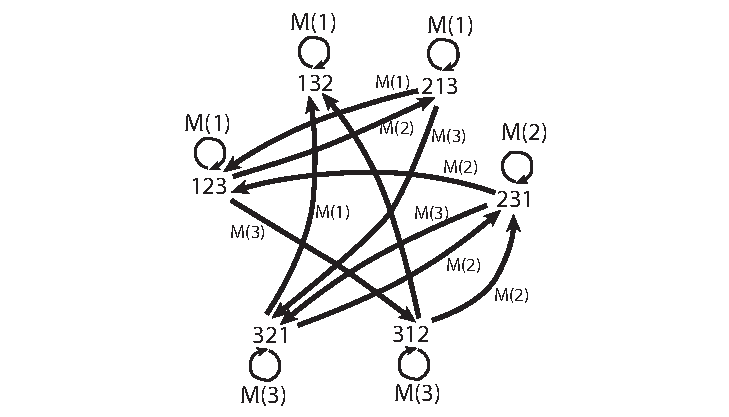
\includegraphics{pics/tr-markov}
\caption{P�echody mezi stavy}
\label{tr-markov}
\end{figure}


Tyto Markovovy �et�zce jsou nerozlo�iteln� a aperiodick� a to znamen�, �e
existuj� asymptot. pravd�podobnosti, tj. pro seznam $\Pi$ je d�na
pravd�podobnost ${\kappa}_{\Pi}$, �e po proveden� n�hodn� posloupnosti $P$ s
dan�m rozlo�en�m operac� skon��me u seznamu $\Pi$.
\par

Pak o�ek�van� �as je $\sum_{\Pi}{\kappa}_{\Pi}\sum_{i}{\beta}_i\Pi(i)$, 
$\Pi(i)$ je pozice $i$ v seznamu $\Pi$.
\par
$p_1 = \sum_{\Pi}{\kappa}_{\Pi}\Pi(i)$ ... o�ek�van� pozice prvku $i$
\par
$\delta(j,i)$ = asmyptot. pst., �e prvek $j$ je p�ed $i$, pak plat� \\
$$
\delta(j,i) = \sum\{\kappa_\Pi , \Pi\ seznam, \Pi(j) < \Pi(i)\}
$$

pak 
\begin{equation}
\begin{split}
p_i & = \sum_{\Pi}\kappa_\Pi\Pi(i) \\
& = \sum_{\Pi}\kappa_\Pi(1 + |{j, \Pi(j) < \Pi(i)|} \\
& = 1 + \sum{j,\Pi}\{\kappa_\Pi, \Pi(j) < \Pi(i)\} \\
& = 1 + \sum_{j}\delta(j,i) (1)
\end{split}
\end{equation}

Zkus�me $\delta(j,i)$ spo��tat jin�m zp�sobem: \\
Idea: jak se m��e st�t, �e ve v�sledn�m seznamu je $j$ p�ed $i$ ?
V posloupnosti $P$ existovala operace MEMBER($x$) a po n� se u� nevyskytovala
operace MEMBER($i$) ani MEMBER($j$).
\par

Jak� je pravd�podobnost tohoto jevu ?
\begin{multline}
\beta_j\sum_{k=0}^{\infty}[1 - (\beta_i - \beta_j)]^k 
= \beta_j \frac{1}{1-(1-(\beta_i+\beta_j)} 
= \frac{\beta_j}{\beta_j+\beta_i} \stackrel{(1)}{=} 
1 + \sum_{\substack{j,i\\j \ne i}} \frac{\beta_j}{\beta_j+\beta_i}
\end{multline}

O�ek�van� �as operace \mnote{jake operace ? XXX} je 
$$
\sum_{i} \beta_i p_i 
= \sum_{\substack{j,i\\j \ne i}} \frac{\beta_i\beta_j}{\beta_i+\beta_j}
$$

P�edpokl�dejme, �e $\beta_1 \geq \beta_2 \geq ... \geq \beta_n$ \\
pak nejrychlej�� algoritmus na seznam $x_1 - x_2 - ... - x_n$ je klasick�
algoritmus bez p�em�s�ov�n� prvk�. Klasick� algoritmus je takov�
algoritmus, kter� p�edem v�, jak� jsou pravd�podobnosti
p��stupu k jednotliv�m prvk�m a m� p�edem seznam srovnan� 
sestupn� podle t�chto pravd�podobnost�.
\par
O�ek�van� �as tohoto algoritmu je 

\begin{equation}
\begin{split}
\sum_{i=1}^{n}i\beta_i 
& = 1 + \sum_{i,j=1} 2\frac{\beta_j\beta_i}{\beta_i+\beta_j} \\
& \leq 1 + \sum_{\substack{i,j\\j<i}} 2\beta_i 
= 1 + \sum_{i=1}^{n} 2(i-1)\beta_i \\
& = 1 + 2\cdot\sum_{i}i\beta_i - 2\sum_{i}\beta_i \\
& = 2\sum_{i=1}^{n}i\beta_i - 1
\end{split}
\end{equation}

Plat�
$$
\frac{\beta_j}{\beta_j+\beta_i} \leq 1
$$


% Splay stromy -------------------------------------------------------------

\section{Splay stromy}
% thanks to Jana Skot�kov� & Martin Mal� za z�pisky, p�epsal Vladim�r Kotal

% \mnote{��ste�n� p�evzato z text� FIT VUTBR}

Splay strom (splay tree, rozvinut� strom) pat�� do kategorie 
adaptabiln�ch datov�ch struktur ur�en�ch k vyhled�v�n�. M� z�kladn� 
vlastnosti bin�rn�ch vyhled�vac�ch strom� - obsahuje ohodnocen� prvky. 
Ka�d�mu reprezentovan�mu prvku $s \in S$, kde $S \subseteq U$, 
($U$ je universum) je p�i�azena v�ha.
\par
V pr�b�hu operac� nad touto strukturou se v�ak m�n� jej� uspo��d�n� 
ve prosp�ch celkov�ho sn��en� �asov� slo�itosti.


\subsection{Operace SPLAY}

Z�kladn� operac� je pro pr�ci s t�mito stromy je SPLAY($x$) - roz���en�, 
kter� zjist�, zda $x$ je reprezentov�n v dan� mno�in�. 
Pokud x le�� v mno�in�, algoritmus ho p�em�st� do ko�ene.

Kdy� $x$ nele�� v mno�in�, pak algoritmus p�em�st� do ko�ene bu� nejmen��
prvek v�t�� ne� $x$ nebo nejv�t�� prvek men�� ne� $x$ (kter� le�� v reprez.
mno�in�)

Tento mechanismus 
se za��n� od stanoven�ho uzlu, a postupn�mi rotacemi zp�sobuje, �e 
stanoven� uzel se stane ko�enem stromu, p�i zachov�n� vyhled�vac�ch 
relac�. Celkov�m v�sledkem je skute�nost, �e �asto pou��van� polo�ky se 
hromad� v bl�zkosti ko�ene. Na rozd�l od BVS, jeho� nejhor�� p��pad pro 
degenerovan� (line�rn�) strom m� slo�itost $O(N)$ a je slo�itost splay 
stromu pro "$k$" r�zn�ch po sob� jdouc�ch operac� $O(k*\log(N))$. Tato 
slo�itost nen� stanovena tradi�n�m p��stupem "nejhor�� p��pad", kter� hled� 
nejnev�hodn�j�� situaci izolovan� operace, ale metodou "amortizovan� 
anal�zy" (amortized analysis), kter� hodnot� celou sekvenci r�zn�ch 
operac�. N�kter� z nich jsou del��, n�kter� krat�� ne� $\log(N)$, ale v 
pr�m�ru vych�z� slo�itost $O(ln(N))$.

Splay stromy p�edstavuj� jeden z p��klad� adaptabiln�ch datov�ch 
struktur, jejich� vnit�n� uspo��d�n� se m�n� vlivem jako vedlej�� jev 
operac� nad t�moto strukturami. Maj� dobrou tendenci vyva�ovat stromovou 
strukturu a svou vlastnost� p�ibli�ovat �asto vyhled�van� kl��e ko�eni 
se podobaj� adaptibiln� line�rn� struktu�e pro sekven�n� vyhled�v�n�, v 
n�� se ka�d� vyhledan� uzel vym�n� se sv�m lev�m p�edch�dcem. I ve 
stromov� podob� si algoritmus zachov�v� jednoduchost a pr�hlednost. 


\subsection{Podporovan� operace}

MEMBER($x$,$T$), INSERT($x$,$T$), DELETE($x$,$T$), 
JOIN2($T_1$,$T_2$), JOIN3(x, $T_1$, $T_2$) 
(nebo asi taky JOIN3($T_1$, $x$, $T_2$)), SPLIT($x$), 
CHANGEWEIGHT($x$, $\triangle$).

\begin{itemize}
\item JOIN2($T_1$,$T_2$) \\
P�edpokl�d�, �e $\forall$ prvky reprezentovan� $T_1 < \forall$ prvky
reprezentovan� $T_2$, tj. $max T_1 < min T_2$.

V�sledn� strom reprezentuje $T_1 \cup T_2$.

\item JOIN3($T_1$, $x$, $T_2$) \\
P�edpokl�d�, �e $\forall$ prvky reprezentovan� $T_1 < x < \forall$ prvky 
reprezentovan� $T_2$, tj. $max T_1 < x < min T_2$.

V�sledn� strom reprezentuje $T_1 \cup T_2 \cup x$.


\item SPLIT($x$,$T$) \\
V�sledek: strom $T_1$ : $\forall$ prvky $\in T_1 < x$\\
	strom $T_2$: $\forall$ prvky $\in T_2 > x$\\
+ informace, zda $x$ le�el v reprezentovan� mno�in�

\item CHANGEWEIGHT($x$, $\triangle$) \\
Zjist�, zda $x$ le�� ve strom� a pokud ano, pak k jeho v�ze p�i�te
$\triangle$.
\end{itemize}


\subsection{Algoritmus MEMBER}

Mechanismus vyhled�n� (splay search), pracuje stejn� jako u BVS, ale 
po vyhled�n� se aplikuje na vyhledan� uzel mechanismus Splay, jeho� 
v�sledkem je p�esunut� uzlu na m�sto ko�ene. 

Viz algoritmus \ref{alg:splay.mem}

\begin{algorithm}[!htb]
\caption{MEMBER pro Splay stromy}
\label{alg:splay.mem}
\begin{algorithmic}
\STATE SPLAY(x, S)
\IF {x je reprezentov�n v ko�eni}
  \STATE "$x$ je v $S$"
\ELSE 
  \STATE "$x$ nen� v $S$"
\ENDIF
\end{algorithmic}
\end{algorithm}

\subsection{Algoritmus JOIN2}

Viz algoritmus \ref{alg:splay.join2}

\begin{algorithm}[!htb]
\caption{JOIN2($T_1$,$T_2$)}
\label{alg:splay.join2}
\begin{algorithmic}
% oprava by M. Macok (nejmensi -> nejvetsi), argumenty SPLAY()
% oprava by T. Matousek - opracne
\STATE SPLAY($\infty$, $T_1$) // XXX (nejv�t�� ?) nejmen�� prvek \\
\STATE ko�en $T_2$ bude prav� syn ko�ene $T_1$
\end{algorithmic}
\end{algorithm}

Operac� SPLAY se z $T_1$ stane strom, kde prav� syn ko�ene bude list. 
M�sto toho listu nav�s�me strom $T_2$. \\
Pak budou v lev�m podstromu ko�ene tohoto nov�ho stromu v�echny prvky 
men�� ne� hodnota v ko�enu a v prav�m v�echny v�t��, co� chceme.

\begin{figure}[!htb]
\centering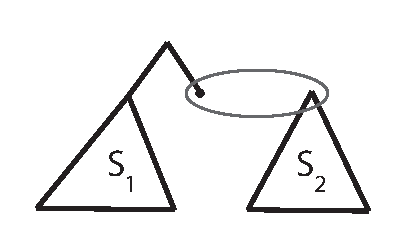
\includegraphics{pics/splay-join2}
\caption{JOIN2 pro splay stromy}
\label{splay-join2}
\end{figure}


\subsection{Algoritmus JOIN3}

Viz algoritmus \ref{alg:splay.join3}

\begin{algorithm}[!htb]
\caption{JOIN3($T_1$, x, $T_2$)}
\label{alg:splay.join3}
\begin{algorithmic}
\STATE vytvo��me vrchol $t$ reprezentuj�c� $x$
\STATE ko�en $T_1$ je lev� syn $t$ \\
\STATE ko�en $T_2$ je prav� syn $t$
\end{algorithmic}
\end{algorithm}

Vytvo��me nov� vrchol reprezentuj�c� $x$ a jeho synov� budou $T_1$ -- lev�,
$T_2$ -- prav�.

\begin{figure}[!htb]
\centering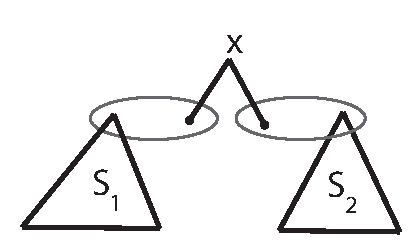
\includegraphics{pics/splay-join3}
\caption{JOIN3 pro splay stromy}
\label{splay-join3}
\end{figure}

\subsection{Algoritmus SPLIT}

Viz algoritmus \ref{alg:splay.split}

\begin{algorithm}[!htb]
\caption{SPLIT($x$,$T$)}
\label{alg:splay.split}
\begin{algorithmic}
%\STATE SPLAY(x)
%\IF {ko�en T reprezentuje x}
%  \STATE $T_1$ podstrom lev�ho syna ko�ene
%       \STATE $T_2$ podstrom prav�ho syna ko�ene
%       \STATE v�stup $T_1$, $T_2$, x, $x \in S$
%  \ELSE
%       \IF {ko�en T reprezentuje prvek $<$ x}
%          \STATE $T_2$ podstrom prav�ho syna ko�ene T
%	       \STATE $T_1 = T - T_2$
%	  \STATE T1 podstrom prav�ho syna ko�ene T
%	       \STATE $T_2 = T - T_1$
%       \ENDIF
%       \STATE v�stup $T_1$, $T_2$, $x \in S$
%\ENDIF
\STATE SPLAY($x$)
\STATE $y$ = prvek reprezentovan� ko�enem
\STATE $T_1$ = podstrom lev�ho syna ko�ene
\STATE $T_2$ = podstrom prav�ho syna ko�ene
\IF {$y = x$}
  \STATE v�stup $T_1$, $T_2$
  \STATE $x \in T$
\ELSIF {$y < x$}
  \STATE v�stup $T \setminus T_2, T_2$
\ELSE
  \STATE v�stup $T_1, T \setminus T_1$
\ENDIF
\STATE $x \not\in T$
\end{algorithmic}
\end{algorithm}

\mnote{zde chybi obrazek, ale celkem nen� pro pochopen� pot�eba :)}


\subsection{Algoritmus DELETE}

Mechanismus ru�en� uzlu (splay delete) je pon�kud slo�it�j��. Uzel, 
kter� se m� zru�it, se mechanismem splay p�esune na pozici ko�ene. 
Zru�en�m ko�ene z�sk�me 2 podstromy. Mechanismus splay se d�le aplikuje 
na bezprost�edn�ho p�edch�dce a nen�-li tak n�sledn�ka zru�en�ho uzlu 
(ve smyslu relace uspo��d�n� - v pr�chodu inorder). T�m se tento uzel 
dostane do pozice ko�ene lev�ho podstromu. Podle pravidel vyhled�vac�ho 
stromu mus� b�t v�echny uzly lev�ho podstromu men�� ne� jeho ko�en a 
v�echny uzly prav�ho podstromu v�t��. Proto mus� m�t lev� podstrom ko�en 
vpravo voln� a na toto m�sto se p�ipoj� prav� podstrom. Tento postup m� 
symetrickou - levou versi. Operace "Splay Delete", ru��c� uzel D XXX je 
uvedena na obr.2.2. XXX
\par
Viz algoritmus \ref{alg:splay.delete}

\begin{algorithm}[!htb]
\caption{DELETE(x)}
\label{alg:splay.delete}
\begin{algorithmic}
\STATE SPLAY(x)
\IF {ko�en reprezentuje x}
  \STATE $T_1$ je podstrom lev�ho syna ko�ene T
       \STATE $T_2$ je podstrom prav�ho syna ko�ene T
       \STATE T $\leftarrow$ JOIN2($T_1$, $T_2$)
\ENDIF
\end{algorithmic}
\end{algorithm}

jin� z�pis:
\begin{algorithmic}
\STATE $T_1, T_2 \leftarrow SPLIT(x, T)$
\STATE $T \leftarrow JOIN2(T_1, x, T_2)$
\end{algorithmic}

\subsection{Algoritmus INSERT}

Mechanismus vkl�d�n� (splay insert) vlo�� uzel jako list stejn�m 
zp�sobem jako BVS, ale potom se aplikuje na vlo�en� uzel mechanismus 
"splay", kter� op�t posune vlo�en� uzel na pozici ko�ene. Operace
"Splay 
insert" uzlu s kl��em C XXX je uvedena na obr. \ref{splay-insert}.
\par


\begin{figure}[!htb]
\centering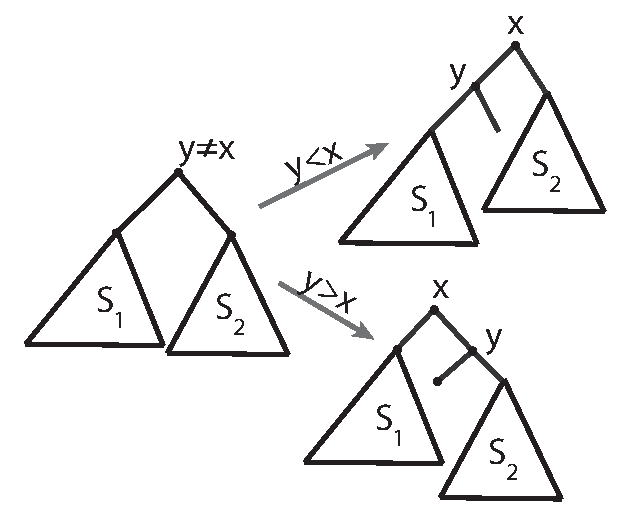
\includegraphics{pics/splay-insert}
\caption{INSERT(x) pro splay stromy}
\label{splay-insert}
\end{figure}


Viz algoritmus \ref{alg:splay.insert}

\begin{algorithm}[!htb]
\caption{INSERT(x)}
\label{alg:splay.insert}
\begin{algorithmic}
\STATE SPLAY(x)
\IF {ko�en nereprezentuje x}
  \IF {ko�en stromu reprez. prvek $<$ x}
          \STATE $T_2$ je podstrom prav�ho syna ko�ene
               \STATE $T_1$ = T - $T_2$ 
	  \ELSE 
	       \STATE T1 je podstrom lev�ho syna ko�ene
	       \STATE $T_2$ = T - $T_1$
       \ENDIF
       \STATE JOIN3($T_1$, x, $T_2$)
\ENDIF
\end{algorithmic}
\end{algorithm}

jin� z�pis:
\begin{algorithmic}
\STATE $T_1, T_2 \leftarrow SPLIT(x, T)$
\STATE $T \leftarrow JOIN3(T_1, x, T_2)$
\end{algorithmic}

\subsection{Algoritmus CHANGEWEIGHT}

Viz algoritmus \ref{alg:splay.chgw}

\begin{algorithm}[!htb]
\caption{CHANGEWEIGHT(x, $\triangle$)}
\label{alg:splay.chgw}

\begin{algorithmic}
\STATE SPLAY(x)
\IF {x je reprezentov�n v ko�eni}
	\STATE k v�ze x p�i�ti $\triangle$
\ENDIF
\end{algorithmic}
\end{algorithm}

P�edpokl�dejme, �e $w(x)$ je v�ha prvku a je to kladn� cel� ��slo.
\par
$tw(x)$ - tot�ln� v�ha $x$, je to sou�et vah v�ech prvk� v podstrom�
ur�en�m $x$.

\begin{priklad}
\mnote{chyb� obr�zek, tady je to nejake zmatene}
% XXX obr

$tw(a) = w(a) + w(b) + w(c)$ \\

$r(x)$ je $rank(x)$ \\
$r(x) = \lfloor \log tw(x) \rfloor$

$bal(konfigurace) = \sum \{ r(x) : x \in konfigurace \}$

Pro strom $T$ je $tw(x) = tw(\text{ko�en }T)$ \\
	       $r(T) = r(\text{ko�en }T)$
\end{priklad}

\begin{lemma}
Nech� $T$ je bin�rn� vyhled�vac� strom, $t$ je vnit�n� vrchol a $u$,$v$ jsou
synov� $t$. Pak $r(t) > min\{r(u), r(v)\} (r(list) = -\infty)$.
\end{lemma}

\begin{proof}
P�edpokl�dejme, �e $tw(u) \leq tw(v)$\\
$$
r(t) = \lfloor \log tw(t) \rfloor \geq \lfloor \log 2tw(u) \rfloor =
1 + \lfloor \log tw(u) \rfloor = 1 + r(u)
$$
\end{proof}

\subsection{Algoritmus SPLAY}

Vol�n� algoritmu SPLAY se v�t�inou zapisuje jako SPLAY($x$), kde explitictn�
neuv�d�me strom, na kter�m je operace prov�d�na - to v�t�inou vyplyne z
kontextu. Tam, kde je nutn� uv�st, na kter�m strom� se operace SPLAY
prov�d� (nap�. v implementaci operace JOIN2, p��eme vol�n� jako 
SPLAY($x$,$T$).

Viz algoritmus \ref{alg:splay.spl}

\begin{algorithm}[!htb]
\caption{SPLAY(x)}
\label{alg:splay.spl}
\begin{algorithmic}
\STATE SPLAY(x)
\STATE $t$ $\leftarrow$ ko�en
\WHILE {$t$ nen� list a $t$ nereprezentuje $x$}
	\IF {$x < t$}
		\STATE $t$ $\leftarrow$ lev� syn $t$
	\ELSE
		\STATE $t$ $\leftarrow$ prav� syn $t$
	\ENDIF
\ENDWHILE
\IF {$t$ je list}
	\STATE $t \leftarrow otec(t)$
\ENDIF
\WHILE {$t$ nen� ko�en}
	\IF {$otec(t)$ je ko�en}
	  \STATE rotace($t$, otec($t$))
	\ELSE
		\IF {otec($t$) i $t$ jsou oba lev� (prav�) synov�}
		  \STATE rotace(otec($t$), d�d($t$))
		  \STATE rotace($t$, otec($t$))
		\ELSE
		  \STATE dvojit� rotace($t$, otec($t$), d�d($t$))
		\ENDIF
	\ENDIF
\ENDWHILE
\end{algorithmic}
\end{algorithm}

V algoritmu
SPLAY (algoritmus \ref{alg:splay.spl}) se pou��v� jednoduch� 
(obr. \ref{splay-rot}) a dvojit� (obr. \ref{splay-dvojrot}) rotace.
Vrchol $t$ se po skon�en� operace SPLAY(x) dostane do ko�ene. Toho
dos�hneme tak, �e v prvn�m cyklu najdeme vrchol $t$ reprezentuj�c� prvek
$x$, v druh�m cyklu p�esouv�me vrchol $t$ do ko�ene.

\begin{figure}[!htb]
\centering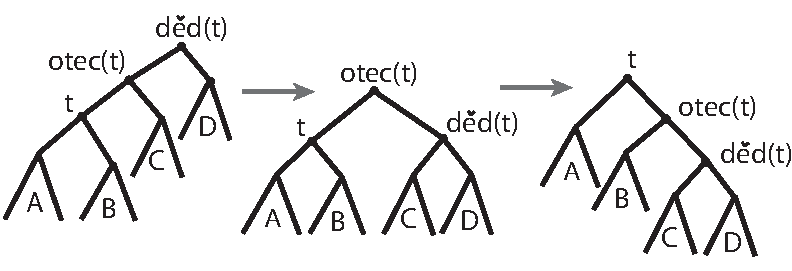
\includegraphics{pics/splay-rot}
\caption{Dvakr�t jednoduch� rotace pro SPLAY($x$)}
\label{splay-rot}
\end{figure}

\begin{figure}[!htb]
\centering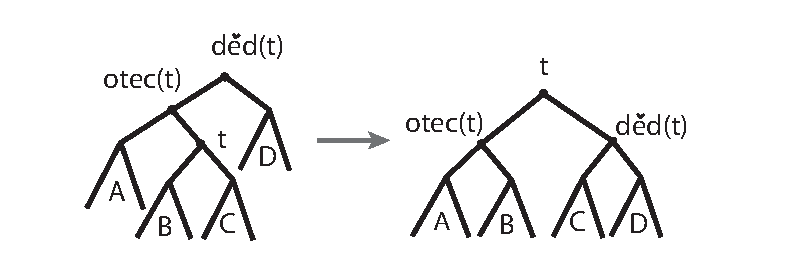
\includegraphics{pics/splay-dvojrot}
\caption{Dvojrotace pro SPLAY($x$)}
\label{splay-dvojrot}
\end{figure}


\subsection{Amortizovan� slo�itost SPLAY}

Budeme p�edpokl�dat, �e $v(x) \geq 1$ pro ka�d� $x$. \\
Tot�ln� v�ha $x = w(x)$, co� je sou�et vah v�ech prvk� v podstromu vrcholu
reprezentuj�c�ho $x$.
\par
Zna��me $r(x) = \lfloor log_2 w(x)\rfloor = \text{rank vrcholu } x$
\par
Pro strom $T$: \\
$$w(T) = w(\text{ko�en}(T)) \\
r(T) = r(\text{ko�en}(T))$$
\par
bal(konfigurace) = sou�et rank� v�ech vrchol� v mno�in�ch tvo��c�ch
konfigurace
\par
N� c�l : Budeme cht�t uk�zat, �e amortizovan� slo�itost operac� je
$O(\log\frac{w(T)}{v(x)})$, kdy� $T$ reprezentuje $S$.
\par
�as operace SPLAY = po�et b�h� druh�ho cyklu, kter� vrchol $t$ 
transportuje do ko�ene.


\begin{lemma}
\label{splay-pomlemma}
Pomocn� lemma: M�jme vrchol $w$ ve strom� $T$ se syny $y_1$ a $y_2$ a
p�edpokl�dejme, �e $y_1$, $y_2$ nejsou listy. Kdy� $w$ reprezentuje $a$,
$y_r$ reprezentuje $b_i$ pro $i=1,2$, pak $rank(a) > min\{r(b_1),r(b_2)\}$
\end{lemma}

\begin{proof}
\begin{figure}[!htb]
\centering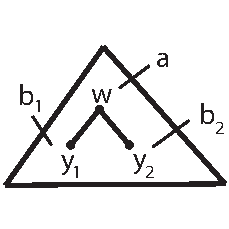
\includegraphics{pics/splay-lemma}
\caption{Pro d�kaz pomocn�ho lemmatu pro splay stromy}
\label{splay-lemma}
\end{figure}

Situaci lze vid�t na obr�zku \ref{splay-lemma}. 
\par
Z�ejm� $r(a) \geq r(b_1)$ a $r(a) \geq r(b_2)$, tedy $r(b_1) \neq r(b_2) 
\Rightarrow r(a) > min\{r(b_1),r(b_2)\}$
\par
\begin{equation}
\begin{split}
r(a) 
& = \lfloor \log_2 w(a) \rfloor \geq \lfloor (w(b_1) + w(b_2)) \rfloor \\
& \geq \lfloor \log_2(2 - min\{w(b_1),w(b_2)\}) \\
& = 1 + \log_2 min\{w(b_1),w(b_2)\} \\
& = 1 + min\{w(b_1),w(b_2)\}
\end{split}
\end{equation}
\end{proof}

\begin{theorem}
Amortizovan� slo�itost operace SPLAY($x$,$T$) $\leq 3(r(T)-r(t)) + 1$, 
kde $t$ je vrchol, kter� transportujeme do ko�ene. $T$ je strom
reprezentuj�c� $S$.
(kdy� $x$ je prvek reprez. mno�iny, pak $t$ reprezentuje $x$, jinak je to bu�
nejv�t�� nebo nejmen�� prvek men�� (v�t��) ne� $x$)
\end{theorem}

\begin{proof}
Ozna�me $T_0$ p�vodn� strom, $T_i$ strom po $i$-t�m b�hu druh�ho cyklu 
v SPLAY a
p�edpokl�dejme, �e druh� cyklus b�� k-kr�t. (tj. $T_k$ je v�sledn� strom)
\par
Amortizovan� slo�itost (SPLAY($x$,$T$)) 
\mnote{$\text{"�as operace" } = k$}
\begin{equation}
\begin{split}
& = \text{�as operace} + bal(\text{v�sledn� konfigurace}) - 
bal(\text{p�vodn� konfigurace}) \\ 
& = k + bal(T_k) - bal(T_0) \\
& = \sum_{i=1}{k}(1 + bal(T_i) + bal(T_{i-1})
\end{split}
\end{equation}
\mnote{$balance = \sum \text{rank v }T_k$}

Ozna�me $r_i$ rank ve strom� $T_i$, nech� $u_i$ je otec $t$ ve strom�
$T_i$ a kdy� $u_i$ nen� ko�en $T_i$, pak $v_i$ je otec $u_i$ v $T_i$.

\begin{itemize}
\item a)
$u_i$ je ko�en: \\
chci odhadnout $1 + bal(T_i) - bal(T_{i-1})$ :
\begin{equation}
\begin{split}
& 1 + bal(T_i) - bal(T_{i-1}) \\
& = 1 + \sum_{z \text{ reprezentov�n v }T_i} r_i(z) + \sum_{z} r_{i-1}(z) \\
& = 1 + r_i(u_{i-1}) + r_i(t) - r_{i-1} - r_{i-1}(t) \\
& = 1 + r_i(u_{i-1}) - r_{i-1}(t) 
\leq 1 + 3(r_{i-1}(u_{i-1}) - r_{i-1}(t))
\end{split}
\end{equation}

\begin{figure}[!htb]
\centering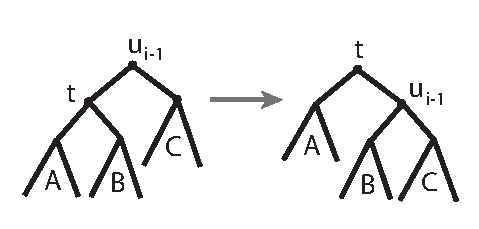
\includegraphics{pics/splay-amortproof1}
\caption{Pro d�kaz amort. slo�itosti operace SPLAY}
\label{splay-amortproof1}
\end{figure}

Plat� $r_i(t) = r_{i-1}(u_{i-1})$, proto�e stromy $A$,$B$,$C$ na obr.
\ref{splay-amortproof1} jsou stejn�.
\par
Plat�
$$
r_i(u_{i-1}) \leq r_{i-1}(u_{i-1}) 
$$
$$
r_{i-1}(u_{i-1}) \geq r_{i-1}(t)
$$

\item b)
  $u_{i-1}$ nen� ko�en: 
  \begin{enumerate}
  \item $u_{i-1}$ je jin� syn v $T_{i-1}$ ne� $t$
  \item $u_{i-1}$ je stejn� syn v $T_{i-1}$ jako $t$
  \end{enumerate}
\end{itemize}

\par
\begin{itemize}
\item ad b1) : \\
\begin{equation}
\begin{split}
& 1 + bal(T_i) - bal(T_{i-1} = \sum_{z}{} r_i(z) - \sum_{z}{} r_{i-1}(z) \\
& = 1 + r_i(t) - r_i(u_{i-1}) + r_i(v_{i-1}) - r_{i-1}(t) - r_i(u_{i-1}) -
	r_{i-1}(v_{i-1}) \\
& = 1 + r_i(u_{i-1}) + r_i(v_{i-1}) - r_{i-1}(t) - r_{i-1}(u_{i-1}) \\
& \leq 2(r_{i-1}(v_{i-1}) - r_{i-1}(t)) \\
& \leq 3(r_{i-1}(v_{i-1}) - r_{i-1}(t))
\end{split}
\end{equation}

Prvn� nerovnost v odvozen� plat�, proto�e 
$1 + r_i(u_{i-1}) + r_i(v_{i-1}) = 2r_{i-1}(t) = 2r_{i-1}(v_{i-1})$.
\par
Amortizovan� slo�itost b�hem cyklu: $\leq 3(r_i(v_{i-1}) - r_{i-1}(t))$

\item ad b2) : \\

$1 + bal(T_i) - bal(T_{i-1}) = ... 
= 1 + r_i(u_{i-1}) + r_i(v_{i-1}) - _{i-1}(t) - r_{i-1}(u_{i-1}) \leq$

  \begin{itemize}
  \item{$\alpha$} \\
    P�edpoklad: $r_{i-1}(t) < r_i(v_{i-1})$ \\
    Pak plat�: \\
    $\leq 1 + 2(r_{i-1}(v_{i-1}) - r_{i-1}(t)) 
    \leq 3(r_i(v_{i-1}) - r_{i-1}(t))$
  \item{$\beta$} \\
    P�edpoklad: $r_{i-1}(t) = r_i(v_{i-1})$, $r_i(t) > r_i(v_{i-1})$ \\
    $... = 1 + r_i(u_{i-1}) + r_i(v_{i-1}) - r_{i-1}(t) - r_{i-1}(u_{i-1})
    \leq 2(2(r_{i-1}(v_{i-1}) - r_{i-1}(t))
    \leq 3(r_i(v_{i-1}) - r_{i-1}(t))$
  \item{$\gamma$} \\
    P�edpoklad: $r_i(t) = r_i(v_{i-1}) - r_{i-1}(v_{i-1}) = r_{i-1}(t)$ \\
    V�m: $r_{i-1}(t) = r'(t) = r_{i-1}(v_{i-1}) = r'(u_{i-1}) 
    = r_i(t) = r_i(v_{i-1}) = r'(v_{i-1})$
    spor s lemmatem \ref{splay-pomlemma}.
    $\Rightarrow$ p��pad $\gamma$ nem��e nastat
  \end{itemize}

  Z�v�r pro b) : Amortizovan� slo�itost b�hem cyklu 
  $\leq 3(r_i(v_{i-1}) - r_{i-1}(t))$

\end{itemize}

V�dy plat� $r_i(v_{i-1}) = r_i(t)$ \\
\begin{equation}
\begin{split}
& \sum_{i=1}{k}(1 + bal(T_i) - bal(T_{i-1})) \\
& \leq \sum_{i=1}{k} 3(r_i(v_{i-1}) - r_{i-1}(t)) \\
& = 1 + 3(r_{k-1}(v_{k-1}) - r_0(t)) = 1 + 3(r_o(T) - r_0(t))
\end{split}
\end{equation}


%
% XXX toto je puvodni dukaz jsem napsal nekdy v 2003:
%
%rozd�l�me podle akce, kter� se prov�d� ve while cyklu
%\begin{itemize}
%\item while cyklus prov�d� rotace
%
%$= 1 + r'(u) - r(v) \leq 1 + r(u) + r(v)$ \\
%$\leq 1 + 3(r(u) - r(v))$
%
%proto�e $x$ m� v p�vodn�m i nov�m strom� stejn� prvky
%\mnote{ne�iteln�}
%$r(u) = r'(t)$ \\
%$r'(u) \leq r'() = r(u)$
%
%\par
%% b)
%\item while cyklus prov�d� dvojitou rotaci
%
%\mnote{tady chybi obr.}
%
%\begin{multline}
%\label{amort-dvojrotace}
%\text{Amortizovan� slo�itost t�to operace} \\
%\text{= �as operace + bal(nov� konf.) - bal(p�vodn� konf.) =} \\
%= 1 + r'(u) - r(v) - r(u) - r(t)
%\end{multline}
%
%pro $x \neq t,u,v$ plat� $r(x) = r'(x)$ \\
%$r(v) = r'(t)$
%
%\begin{itemize}
%  \item
%  \begin{multline}
%  r(v) > r(t), pak r'(u),r'(v) \leq r'(t) = r(v)\\
%  r(u) \geq r(t), 1 \leq r(v) - r(t) \stackrel{\text{ \ref{amort-dvojrotace}
%  }}{\leq} \\
%  r(v) - r(t) + 2r(u) - 2r(t) = 3(r(v) - r(t))
%  \end{multline}
%  
%  \item
%  r(v) = r(t), pak podle lemmatu $r'(t) > min\{r'(u), r'(v)\}$ plati \\
%  \begin{multline}
%  2r'(t) \geq r'(u) + r'(v) + 1 
%    \stackrel{\text{ \ref{amort-dvojrotace} }}{\leq} \\
%  2r(u) - 2(r(t) = 2(r(v) - r(t)) = (r(t) = 0) 3(r(u) - 3r(t))
%  \end{multline}
%  
%\end{itemize}
%\end{itemize}

\end{proof}




% -------------------------------------------------------------------------

\subsection{Amortizovan� slo�itost ostatn�ch operac�}

\begin{defn}
Amortizovan� slo�itost operace $SPLAY(x,T) \leq 1 + 3(r(T)-r(t))$, kde $t$
je prvek, kter� se p�em�st� do ko�ene.
\end{defn}

\par
Ozna�me $t_{-}$ prvek ve strom� T, kter� reprezentuje nejv�t�� prvek 
$\leq x$.
\par
Ozna�me $t_{+}$ prvek ve strom� T, kter� reprezentuje nejmen�� prvek 
$\geq x$.
\par
Kdy� $x$ je reprezentov�no $T$, pak $t_{-} - t_{+}$ je prvek reprezentuj�c�
$x$.
\par
Jednotliv� operace maj� n�sleduj�c� amortizovan� slo�itosti:

\begin{itemize}
\item $SPLAY(x,T) = O(\log\frac{w(T)}{min\{w(t_{-}),w(t_{+})\}})$ \\
\item $MEMBER(x,T) = O(\log\frac{w(T)}{min\{w(t_{-}),w(t_{+})\}})$ \\
\item $SPLIT(x,T) = O(\log\frac{w(T)}{min\{w(t_{-}),w(t_{+})\}})$ \\
\item $CHANGEWEIGHT(x, \triangle) = O(\log\frac{
w(T) - max\{\triangle,0\}}{min\{w(t_{-}),w(t_{+})\}
})$ \\
\item $JOIN3(T_1, x, T_2) = O(\log\frac{w(T_1)+w(T_2)+v(x)}{v(x)})$
\end{itemize}

Ozna�me $t_{\infty}$ prvek v $T_1$, kter� reprezentuje nejv�t�� prvek z
$T_1$. Pak amortizovan� slo�itosti pro zb�vaj�c� operace jsou
n�sledujic�:
\par

\begin{itemize}
\item $JOIN2(T_1,T_2) = O(\log\frac{w(T_1) + w(T_2)}{w(t_{\infty})})$ \\
\item $DELETE(x,T) = O(\log\frac{w(T)}{min\{w(t_{-}),w(t_{+}),w(t_{1}\}})$ \\
\end{itemize}

Prvek $t_1$ je prvek $T_1$, kter� reprezentuje v $T$ nejv�t�� prvek $\leq x$.

\begin{itemize}
\item $INSERT(x,T) = O(\log\frac{w(T) + v(x)}{min\{w(t_{-}),w(t_{+})\}})$
\end{itemize}

% priklad pro SPLAY stromy ----------------------------------------------

\begin{priklad}
M�jme mno�inu $X={x_1,...,x_n}$ a pravd�podobnosti pro v�skyt operace
MEMBER(x). Nech� $U$ je optim�ln� bin�rn� vyhled�vac� strom. Nech� $T$ je
bin�rn� vyhled�vac� strom reprezentuj�c� $X$. $P$ je posloupnost operac�
MEMBER(x) vyhovuj�c� dan�m pravd�podobnostem.
\par
Chceme aplikovat $P$ na strom $T$, kde pro implementaci pou�ijeme strategii
SPLAY strom�.
\par
Srovn�me �as, kter� tato strategie vy�aduje s �asem obvykl� implementace
MEMBER p�i aplikaci $P$ na $U$.
\par
Definujeme $v(x) = 3^{d-d(x)}$, kde d je hloubka stromu $U$ a $d(x)$ je
hloubka prvku v $U$ reprezentuj�c�ho prvek $x$.
\par
Spo��t�me tot�ln� v�hu prvku $x$:
$$w(x) = \sum_{i=0}{d-d(x)} 2^i3^{d-d(x)-i} 
\leq 3^{d-d(x)} \sum_{i=0}{d-d(x)} (\frac{2}{3})^i \leq 3^{d-d(x)+1}$$
\par
Pak plat�: \\
$r(x) \leq d-d(x)+1$ \\
$r(T) \leq d+1$, (prvek v ko�eni m� hloubku $0$)
\par
Amortizovan� slo�itost operace MEMBER(x) 
$$\leq O(d(x)) = 
O(r(T)-r(x)) = O(d+1-d+d(x)-1) = O(d(x))$$
\par
�as posloupnosti $P$ pou�it� na strom $T$ a implementovan� strategi� SPLAY 
$$= (\sum_{\text{operace v P}}{} \text{amortizovan� slo�itost operac� v P}) +
bal(T) = O(\text{�as P pro strom U} + bal(T))$$
\par
$bal(T)$ je balance stromu $T$. 
$$bal(T) = \sum_{x \in X}{} r(x) = 
\sum_{x \in X}{} d+1 = O(x^2)$$
\par
$$\Rightarrow  O(\text{�as P pro strom U}) + bal(T) = 
O(\text{�as P pro U} + x^2)$$
\mnote{tady bylo ve vzorci n�co jako $|x^2|$ (?)}
\par
Z�v�r: pro dlouh� posloupnosti snad t�m�� stejn� jako opt. BVS.
\end{priklad}

% EOF

% ==========================================================================
% ==========================================================================
% prednaska DS 7.4.2003

\chapter{Haldy}

\begin{defn}
Haldy jsou stromov� struktury, kter� spl�uj� 
\begin{itemize}
\item lok�ln� podm�nku na uspo��d�n�
  - prvek reprezentuj�c� otce je men�� ne� prvek reprezentovan� synem
    apod.
% oprava by M. Macok:
% "strukturalni podminky" na stromy jsou podminky na tvar
% stromu (event. lesu), podle kterejch se ty haldy rozdelujou na Fib.,
% leftlist apod... neni tam nic o tom, jestli jsou synove vetsi/mensi
% nez otcove apod., od toho je tam ta prvni podminka...
\item struktur�ln� podm�nku na stromy, ze kter�ch jsou vytvo�en� 
\end{itemize}
\end{defn}

\begin{pozn}
podle t�chto podm�nek se haldy rozd�luj� na Fibonacciho, Leftist,
d-regul�rn� apod. (mohou se li�it jak lok�ln�, tak struktur�ln� podm�nkou)
\end{pozn}

% --------------------------------------------------------------------------
\section{$d$-regul�rn� haldy}

\begin{defn}
d-regul�rn� halda, d cel� ��slo d$\geq$ 2 \\
Je to strom T takov�, �e existuje jednozna�n� korespondence mezi vrcholy
strom� a prvky reprezentovan� mno�iny a plat�: 
\begin{enumerate}

\item strom T spl�uje struktur�ln� podm�nky
\begin{enumerate}
\item ka�d� vrchol s vyj�mkou nejv��e jednoho je bu� list nebo m� d syn�
\item ka�d� vrchol m� nejv��e d syn�
\item existuje o��slov�n� syn� ka�d�ho vrcholu tak, �e po o��slov�n�
pr�chodem ���ky plat�: \\
kdy� vrchol nen� list, pak ka�d� vrchol s men��m ��slem m� d syn�.
\end{enumerate}

\item podm�nku na lok�ln� uspo��d�n�: \\
kdy� x je prvek p�i�azen� vrcholu t, pak otci(t) je p�i�azen prvek
$\leq$ x
pak po o��slov�n� pr�chodem do ���ky plat�:
kdy� vrchol m� ��slo i, jeho synov� maj� ��sla
% oprava by M.Macok :
% strana 70, prvni syn vrcholu neni na pozici d(i-1)+1 ale ..+2
d(i-1)+2,d(i-1)+3,...,di+1 a otec m� ��slo 
$\lceil\frac{i-1}{d}\rceil$.
\end{enumerate}
\end{defn}

P�. 3-regul�rn� halda

% obr.

kdy� takto o��slovan� prvky d�me do pole, pak plat�: kdy� je vrchol na
i-t�m m�st�, ��sla syn� jsou 3(i-1)+2, 3i, 3i+1
a otec je na $\lceil\frac{i-1}{3}\rceil$ m�st� v poli.
to vyu�ijeme pro implementaci polem - u�et��me m�sto.
\par

\begin{pozn}
nejpopul�rn�j�� jsou 2-reg. haldy, proto�e synov� i-t�ho vrcholu
jsou na m�stech $2(i-1)+2=2i, 2(i-1)+3=2i + 1$, otec je na
$\lceil\frac{i-1}{2}\rceil + 1 = \lceil\frac{i}{2}\rceil$. 
$\Rightarrow$ snadn� po��t�n� (bitov� posun)
\end{pozn}

\subsection{Algoritmus UP}
UP(x) ... srovn� haldu sm�rem nahoru

A: if prvek reprezentovan� x je $<$ prvek reprezentovan� otcem(x) then
  x a otce(x) vym�n�me a pokra�ujeme v A


\subsection{Algoritmus DOWN}

A: if prvek reprezentovan� x $>$ prvek reprezentovan� n�kter�m synem x
then vym�n�me x a syna x, kter� reprezentuje nejmen�� prvek, pokra�ujeme
v A

\begin{pozn}
kdy� m� hlada hloubku h, pak UP(x) vy�aduje �as O(h), DOWN(x) �as
O(dh).
\end{pozn}

\subsection{Operace na hald�}

\subsubsection{INSERT}
p�id�me posledn� list t reprezentuj�c� x
UP(t)

\subsubsection{MIN}
... prvek reprezentovan� v ko�eni

\subsubsection{DELETEMIN}
prvek reprezentovan� posledn�m listem d�me do ko�ene, odstran�me posledn� list \\
DOWN(ko�en)

\subsubsection{DECREASEKEY$(x, \Delta)$}
mus�me zn�t polohu vrcholu t reprezentuj�c�ho x, toto halda neumo��uje nal�zt. \\
zm�n�me uspo��d�n� v bod� x \\
UP(x) mohl by b�t men�� ne� jeho otec, proto provedeme UP \\

\subsubsection{INCREASEKEY$(x, \Delta)$}
mus�me zn�t polohu vrcholu t reprezentuj�c�ho x, toto halda neumo��uje nal�zt \\
zm�n�me uspo��d�n� v bod� x \\
DOWN(x)

\subsubsection{DELETE}
Mus�me zn�t polohu vrcholu t reprezentuj�c�ho x, toto halda neumo��uje
nal�zt \\
Vezmeme prvek y reprezentovan� posledn�m listem, odstran�me posledn� list,
prvek t, kter� reprezentoval x bude reprezentovat y

\begin{algorithmic}
\IF {y $<$ x} 
  \STATE UP(t) else DOWN(t) 
\ENDIF
\end{algorithmic}

\subsection{Algoritmus MAKEHEAP}
D�na prost� posloupnost $x_1, x_2, ..., x_n$.
Chceme vytvo�it d-reg. haldu reprezentuj�c� mno�inu 
${ x_1, x_2, ..., x_n }$. Vezmeme "d-reg. strom" T s vrcholy p�i�ad�me
prvky $x_1, x_2, ..., x_n$. Pro v�echny vrcholy, kter� nejsou listy podle
o��slov�n� v po�ad� od nejv�t��ho k nejmen��mu provedeme DOWN(t).
\par

\mnote{chyb� obr�zek}
% XXX obr.

Invariant: v okam�iku, kdy prov�d�m DOWN(t), tak vrcholy, kter�
reprezentuj�c� v�t�� prvky spl�uj� sm�rem dol� podm�nku 

\subsection{Slo�itost operac�}
V d-reg. hald� reprezentuj�c� n-prvkovou mno�inu implementace operac�
vy�aduje �asy dan� tabulkou: \\
\par

\begin{tabular}{|l|l|}
\hline
Operace & slo�itost \\
\hline
MIN & O(1) \\
INSERT, DECREASEKEY & $O(log_d(n))$ \\
DELETEMIN, INCREASEKEY, DELETE & $O(d \cdot log_d(n))$ \\
\hline
\par
\end{tabular}
\\

M�me vrchol v i-t� hladin� a "d-reg. strom" m� hloubku h. 
Kolik �asu pot�ebuje DOWN(t) ?
Je to O(d(h-1))
po�et vrchol� v i-t� hladin� je di �as MAKEHEAP je 
$O(\sum{i=0}{h-1} d^id(h-i)) = O(dS)$, kde 
$$
S = \sum{i=0}{h-1}d^i(h-i)
$$
Budeme po��tat 
\begin{multline}\bigparens
dS - S = \sum{i=0}{h-1}d^{i+1}(h-i) - \sum{i=0}{h-1}d^{i}(h-i) = \\
d^h - h + \sum{i=0}{h-1}d^{i}(h-i-(h-i-1)) = d^h - h\frac{d^h - 1}{d-1} \\
\Rightarrow S = \frac{d^h - h}{d-1} + d\frac{d^{h-1} - 1}{(d-1)^2}, 
h = log_d(n) \Rightarrow S \approx O(\frac{n}{d})
\end{multline}


\subsection{Dijkstr�v algoritmus}

K �emu jsou d-reg. haldy dobr� ? nap�. pro implementaci Dijkstrova
algoritmu.
\par

Vstup: orientovan� graf (V,E), fce $c:E \rightarrow R^+$, vrchol z \\
V�stup: $d(v)$, $v \in V$ \\
	$d(v)$ je d�lka nejkrat�� cesty ze $z$ do $v$ \\

\begin{algorithm}[!htb]
\caption{Dijkstra pro d-regularni haldy}
\label{alg:heaps.d-reg.dijkstra}
\begin{algorithmic}
\STATE $d(z) = 0, d(v) = \infty \forall v \in V, v \neq z, U = {z}$\\
\WHILE {$U \neq \emptyset$}
  \STATE vezmeme z U prvek $u \in U$ s nejmen�� hodnotou d(u),
    \STATE odstran�me ho z U.
  \FOR {$\forall(u,v) \in E$}
    \IF {$d(v) > d(u) + c(u,v)$} 
       \STATE $d(v) = d(u) + c(u,v)$ , v p�id�me do U
    \ENDIF
  \ENDFOR
\ENDWHILE
\end{algorithmic}
\end{algorithm}
\par

U reprezentujeme pomoc� d-reg. haldy. Pak �as Dijkstrova algoritmu je 
O($|V| \cdot$ �as na INSERT + $|V| \cdot$ �as na DELETEMIN + $|E| \cdot$ �as na
DESCREASEKEY) 
\par

kdy� d = 2, pak to je $O(|E|log_2(|V|))$
$d = max {\frac{|E|}{|V|}, 2}$, vyjde �as $O(|E|log_d(|V|))$ \\
kdy� $\exists \epsilon$ , �e $|E| \geq c|V|^{1+\epsilon}$ pro n�jak� cc,
pak �as je $O(|E|)$. (graf je dostate�n� hust�) \\
$|E| \geq c|V|\log^{\epsilon} |V|$ pro n�jak� c, $\epsilon$, pak �as
$O(|E|\log log |V|)$.
\par

Dal�� aplikace: t��d�n� \\

HEAPSORT - viz. alg. \ref{alg:heaps.d-reg.heapsort} \\
Vstup: prost� posloupnost prvk� $x_1, x_2, ..., x_n$. \\
V�stup: uspo��dan� psl. pvrk� $x_1, x_2, ..., x_n$. \\

\begin{algorithm}[!htb]
\caption{Heapsort pro d-regularni haldy}
\label{alg:heaps.d-reg.heapsort}
\begin{algorithmic}
\STATE MAKEHEAP($x_1, x_2, ..., x_n$)
  \STATE i = 1
  \WHILE {$HEAP \neq \emptyset$}
    \STATE $x_1$ = MIN(HEAP)
    \STATE DELETEMIN(HEAP)
    \STATE i = i + 1
  \ENDWHILE
\end{algorithmic}
\end{algorithm}
\par

\begin{pozn}
Optimum pro d-reg. haldy je n�kde mezi d=6 a d=7.
\end{pozn}

% --------------------------------------------------------------------------
\section{Leftist haldy}

\begin{defn}
LEFTIST strom \\
M�jme bin�rn� strom a pro ka�d�ho syna m�me ur�eno, zda je lev� nebo
prav�. Pro vrchol v definujeme npl(v) jako d�lku nejkrat�� cesty z v do
vrcholu v podstromu v s nejv��e jedn�m synem. \\
Bin�rn� strom je LEFTIST, kdy� \\
a kdy� v m� jednoho syna, pak je to lev� syn
b kd� v m� dva syny, pak npl(lev�ho syna) $\geq$ npl(prav�ho syna)
\end{defn}

\begin{defn}
Cesta $x_1, x_2, ..., x_n$ se naz�v� prav�, kdy� $x_i$ je prav� syn
$x_{i-1}$ pro i=2,3,...,n a $x_n$ nem� prav�ho syna.
\end{defn}
\par

Vlastnosti: 
\begin{enumerate}
\item ka�d� podstrom leftist stromu je leftist 
\item d�lka prav� cesty z $\forall$ vrcholu v je $\leq$ log(po�et vrchol� v
podstromu vrcholu v)
\end{enumerate}

\begin{defn}
Letist halda reprezentuj�c� mno�inu S je leftist strom T s n vrcholy
takov�, �e exzistuje jednozna�n� korespondence mez prvlky S a vrcholy T
takov�, �e $\forall$ v prvek p�i�azen� vrcholu v $\geq$ prvek p�i�ayen�
otci v.
\end{defn}
\par

\begin{defn} 
MERGE($T_1, T_2$) \\
podm�nka: $T_1, T_2$ reprezentuj� disjunktn� mno�iny $S_1, S_2$.
V�sledek: halda reprezentuj�c� $S_1 \cup S_2$.
\end{defn}
\par

\begin{pozn}
podobn� operaci JOIN v AVL stromech (ale...)
\end{pozn}

\begin{algorithm}[!htb]
\caption{MERGE pro leftist haldy}
\label{alg:heaps.leftist.merge}
\begin{algorithmic}
\STATE MERGE($T_1$, $T_2$)
\IF {$T_1$ = 0}
  \STATE MERGE($T_1$, $T_2$) $\rightarrow T_2$ konec 
\ENDIF
\IF {$T_2$ = 0}
  \STATE MERGE($T_1$, $T_2$) $\rightarrow T_1$ konec 
\ENDIF
\IF {ko�en $T_2$ reprezentuje prvek $<$ prvek repr. ko�enem $T_1$}
  \STATE vym�n�me $T_1$ a $T_2$
\ENDIF
\STATE prav� syn ko�ene $T_1 \rightarrow$ MERGE($T_2$, podstrom prav�ho syna ko�ene $T_1$)
\IF {npl(lev�ho syna ko�ene $T_1$) $<$ npl(prav�ho syna ko�ene $T_1$)}
  \STATE prohod�m syny ko�ene $T_1$
\ENDIF
\STATE npl(ko�ene $T_1$) = npl(prav�ho syna ko�ene $T_1$) + 1
\STATE MERGE($T_1$, $T_2$) $\rightarrow T_1$ 
\end{algorithmic}
\end{algorithm}

\begin{pozn}
�asov� slo�itost operace MERGE v leftist hald�ch je $O(log(n_1+n_2))$, kde
$n_1, n_2$ jsou velikosti reprezentovan�ch mno�in.
\end{pozn}

\begin{algorithm}[!htb]
\caption{INSERT pro leftist haldy}
\label{alg:heaps.leftist.insert}
\begin{algorithmic}
\STATE INSERT(x)
\STATE vytvo��me novou haldu $T_1$ reprezentuj�c� pouze prvek x
\STATE T $\rightarrow$ MERGE($T_1$, $T_2$)
\STATE DELETEMIN
\STATE $T_1 \rightarrow$ podstrom lev�ho syna ko�ene T
\STATE $T_2 \rightarrow$ podstrom prav�ho syna ko�ene T
\STATE T $\rightarrow$ MERGE($T_1$, $T_2$)
\end{algorithmic}
\end{algorithm}

\begin{theorem}
Operace MIN v leftist hald�ch vy�aduje �as O(1), operace MERGE, INSERT, a
DELETEMIN vy�aduj� �as O(log n), kde n je po�et prvk� ve v�sledn� hald�.
\end{theorem}

\begin{pozn}
% XXX obr.
koukneme se jak vypad� v�sledn� strom a pod�v�me se na vrcholy, se kter�mi
jsme n�co museli prov�d�t - tyto vrcholy le�� na prav� cest�, tj. je jich
omezen� po�et.
\end{pozn}

\begin{algorithm}[!htb]
\caption{DECREASEKEY pro leftist haldy}
\label{alg:heaps.leftist.decreasekey}
\begin{algorithmic}
\STATE DECREASEKEY(x)
\STATE odtrhneme podstrom $T_1$ vrcholu x, y $\rightarrow$ otec(x)
\STATE $T_2 = T - T_1$
\STATE zmen��me ohodnocen� ko�ene stromu $T_1$
\IF {y m� jen prav�ho syna}
  \STATE  zm�m�me tohoto syna na lev�ho, npl(y) = 0
\ENDIF
\STATE y $\rightarrow$ otec(y)
\WHILE {npl(y) $>$ min{npl(lev� syn y), npl(prav� syn y)} + 1}
  \IF {npl(lev�ho syna y) < npl(prav�ho syna y)}
    \STATE prohod�me syny y
  \ENDIF
  \STATE npl(y) = npl(prav�ho syna y) + 1, y $\rightarrow$ otec(y)
\ENDWHILE
\STATE T $\rightarrow$ MERGE($T_1$, $T_2$)
\end{algorithmic}
\end{algorithm}

\begin{pozn}
npl, kter� jsem musel p�episovat je v�dycky prav� syn
\end{pozn}

\begin{theorem}
Operace DECREASEKEY, INCREASEKEY a DELETE vy�aduj� �as O(log n) v leftist
hald�ch (a po�et prvk� v�sledn� reprez. mno�iny)
\end{theorem}

% --------------------------------------------------------------------------
\section{Binomi�ln� haldy}

jsou zalo�eny na binomi�ln�m rozvoji ��sel, jsou definov�ny na speci�ln�ch
stromech.

% XXX obr.

Vlastnosti strom� $H_i$
\begin{itemize}
\item $H_i$ m� $2^i$ vrchol�
\item hloubka $H_i$ je i
\item ko�en $H_i$ m� i syn�
\item $\forall j < i$ existuje syn ko�ene $H_i$ takov�, �e 
  jeho podstrom je izomorfn� s $H_j$.
\end{itemize}

\begin{proof}
D�kaz: indukc� p�es i (element�rn�)
\end{proof}

\begin{defn}
Binomick� halda je soubor strom� takov�ch, �e
\begin{itemize}
\item ka�d� strom je izomorfn� s n�jak�m $H_i$
\item ��dn� dva stromy nejsou izomorfn�
\item existuje jednozna�n� korespondence mezi vrcholy reprezentovan�
mno�iny a vrcholy strom� takov�, �e prvek odpov�daj�c� otci je men�� ne�
prvek odpov�daj�c� vrcholu.
\end{itemize}
\end{defn}

\subsection{Operace}

\begin{algorithm}[!htb]
\caption{MERGE pro binomialni haldy}
\label{alg:heaps.binom.merge}
\begin{algorithmic}
\STATE MERGE($T_1$, $T_2$)
\STATE ($T_1, T_2$ binom. haldy velikosti $n_1,n_2$)
\STATE $P = 0, i = 0, T = 0$
\WHILE {$i \leq log(n_1 + n_2)$}
  \STATE $S_1$ je strom v $T_1$ izomorfn� s $H_i$ (pokud neexistuje, tak $S_1=0$)
  \STATE $S_1$ je strom v $T_1$ izomorfn� s $H_i$ (pokud neexistuje, tak $S_1=0$)
  % XXX \CASE
     \IF {$S_1, S_2$, P = 0}
       \STATE neprovedeme nic
     \ENDIF
     \IF {jeden strom z $S_1, S_2$, $P$ je nepr�zdn�} 
        \STATE vlo��m tento strom do $T$, $P=0$
     \ENDIF
     \IF {dva stromy z $S_1, S_2$, $P$ jsou nepr�zdn�}
       \STATE spoj�m tyto stromy a v�sledek vzlo��m do $P$
     \ENDIF
     \IF {v�echny stromy z $S_1, S_2$, $P$ jsou nepr�zdn�}
       \STATE vlo��m do $T$, spojen� $S_1, S_2$ vlo��m do $P$
     \ENDIF
  % \ENDCASE
  \STATE $i = i + 1$
\ENDWHILE
\end{algorithmic}
\end{algorithm}

\begin{pozn}
$P$ odpov�d� p�enosu v bin�rn�m s��t�n�, $T$ je v�sledn� halda.
\end{pozn}

\begin{algorithm}[!htb]
\caption{Spojen� dvou binom. hald}
\label{alg:heaps.binom.spoj}
\begin{algorithmic}
\STATE Spojeni($S_1$, $S_2$)
\STATE $S_1, S_2$ jsou stromy izomorfn� s $H_i$ pro n�jak� $i$
\IF {prvek reprezentovan� ko�enem $S_1 \leq$ prvek reprezentovan� ko�enem $S_2$}
  \STATE ko�en $S_2$ se stane dal��k synem ko�ene $S_1$
\ELSE
  \STATE ko�en $S_1$ se stane dal��k synem ko�ene $S_2$
\ENDIF
\end{algorithmic}
\end{algorithm}

\begin{pozn}
INSERT - stejn� jako v leftist hald�ch \\
MIN - prohled�me prvky reprezentovan� ko�eny strom� a najdeme nejmen��
\end{pozn}

\begin{algorithm}[!htb]
\caption{DELETEMIN pro binom. haldu}
\label{alg:heaps.binom.deletemin}
\begin{algorithmic}
\STATE DELETEMIN
\STATE prohled�n�m prvk� reprezentovan�ch ko�eny strom� naleznu strom $S$,
jeho� ko�en reprezentuje nejmen�� prvek
\STATE $T_1 = T \ {S}, T_2$ je tvo�en podstormy v�echn syn� ko�ene S
\STATE (tj. utrhnu ko�en a zbytek d�m do haldy) - 
	je to halda d�ky vlastnosti 4
\STATE $T \rightarrow$ MERGE($T_1, T_2$)
\end{algorithmic}
\end{algorithm}

\begin{pozn}
Operace DELETE se ned� rozumn� prov�st, museli bychom p�ebudovat cel�
strom.
\end{pozn}

\begin{theorem}
Operace MERGE, INSERT, MIN, DELETEMIN a DECREASEKEY vy�aduj� �as $O(log n)$.
Operace INCREASEKEY vy�aduje �as $O(log^2 n)$.
\end{theorem}

\begin{pozn}
XXX
S��t�n� v bin�rn�ch ��slech m� (XXX amort?) slo�itost $O(1)$.
\\
1 0 0 ... 0 \\
1 1 1 ... 1 \\
\\
amort. slo�. \\
Neplat� n�co podobn�ho pro binom. stromy ? Ano, pro operaci INSERT.
\end{pozn}

\begin{theorem}
Amortizovan� slo�itost operace INSERT je O(1).
\end{theorem}

\begin{pozn}
MERGE zab�r� dost �asu - mus�me ho d�lat ?
\end{pozn}


\subsection{L�n� implementace binom. hald}
Zm�n�me definici - vynech�me podm�nku 2, tj. te� v na�� binom. hald�
mohou b�t izomorfn� stromy.
\par
Operace MERGE($T_1, T_2$) - provedeme konkatenaci seznam� $T_1 a T_2$.
Jenom to by nefungovalo, mus�me je�t� zm�nit operace MIN, DELETEMIN.

\begin{algorithm}[!htb]
\caption{DELETEMIN pro line binom. haldy}
\label{alg:heaps.binom-line.min}
\begin{algorithmic}
\STATE MIN
\STATE p�i prohled�v�n� prvk� reprezentovan�ch ko�eny strom� se�ad�me
stromy do mno�in $Q_i$, $i=0,...,n$ , kde $Q_i$ je mno�ina v�ech strom� v
$T$ izomorfn�ch s $H_i$.
\STATE $i = 0, T = 0$
\WHILE {$\exists Q_i \neq 0$}
  \WHILE {$|Q_i| > 1$}
    \STATE vezmeme dva stromy z $Q_i$, spoj�me je, v�sledek d�me do $Q_{i+1}$
  \ENDWHILE
  \IF {$Q_i \neq 0$}
    \STATE strom z $Q_i$ d�m do $T$
  \ENDIF
  \STATE $i = i + 1$
\ENDWHILE
\end{algorithmic}
\end{algorithm}

DELETEMIN
d� stromy po odtr�en� nejmen��ho prvku do odpov�daj�c�ch mno�in $Q_i$

\begin{theorem}
Operace MERGE a INSERT p�i l�n� implementaci vy�aduj� �as O(1), operace
DELETEMIN a MIN vy�aduj� �as $O(\text{po�et strom�})$.
\end{theorem}

\begin{pozn}
$bal(\text{konfigurace}) = \text{po�et v�ech strom� ve v�ech hald�ch v
konfiguraci}$
\end{pozn}

\subsubsection{Amort. slo�.}
$\text{amort. slo�.} = \text{�as pro operaci} + 
bal(\text{v�sledn� konfigurace}) - bal(\text{p�vodn� konfigurace})$

\begin{tabular}{ll}
MERGE & $O(1)$ \\
INSERT & $O(1)$ \\
MIN & $O(log n)$ \\
DELETEMIN & $O(log n)$ \\
\end{tabular}

\subsection{Zobecn�n� binomi�ln� haldy}

XXX
\mnote{p�edn�elo se to tento rok (2004) v�bec ?}

% --------------------------------------------------------------------------
\section{Fibonacciho haldy}

XXX dopsat !



% ==========================================================================
% Sou��st skript na Datov� struktury. Viz main.tex
\markright{$ $Id$ $}
% p�epsal Vladim�r Kotal

\chapter{Dynamizace}

V uspo��dan�m poli um�me rychle vyhled�vat, ale p�idat prvky znamen�
cel� ho p�ebudovat. Ve str�staj�c�m ha�ov�n� zase ne�ly prvky mazat,
ve velmi komrimovan�ch trie ani p�id�vat, ani mazat. V t�to kapitole
uk�eme obecnou metodu, jak tyto probl�my �e�it, podobnou p��stupu u
binomi�ln�ch hald.

% --------------------------------------------------------------------------
\section{Zobecn�n� vyhled�vac� probl�m}

\begin{defn}
\emph{Vyhled�vac� probl�m} je funkce $f: U_1 \times 2^{U_2} \to U_3$, kde
$U_1$, $U_2$ a $U_3$ jsou univerza.
\end{defn}
\begin{defn}
\emph{�e�en� vyhled�vac�ho probl�mu} pro $x \in U_1, A \subseteq U_2$
je nalezen� hodnoty $f(x, A)$.
\end{defn}

\begin{pozn}
Chceme naj�t strukturu, kter� reprezentuje A a algoritmus, kter� pro vstup
$x \in U_1$ spo��t� $f(x, A)$. Takov� struktu�e se ��k� statick� struktura
pro vyhled�vac� probl�m.
\end{pozn}

P�.:
\begin{description}
\item[Klasick� vyhled�vac� probl�m:]

	$U_1 = U_2 = U$, univerzum prvk�;
	$U_3 = \{0, 1\}, A \subseteq U_2$

	$f(x, A) =
	\begin{cases}
	0& \text{kdy� } x \notin A\\
	1& \text{kdy� } x \in A
	\end{cases}$
	(rozlo�iteln�)
\item[Euklidovsk� vzd�lenost bod� v rovin�:]

	$U_1 = U_2 = $ euklidovsk� rovina; 
	$U_3 = \mathbb{R}^+$; 
	$f(x, A) = dist(x,A$ vzd�lenost bodu $x \in U_1$ od mno�iny $A$.
	(rozlo�iteln�, $\oplus$ ... operace min)
\item{Nalezen� p�edch�dce}
	$U_1 = U_2 = U_3$ 
	pro $x \in U_1$ a $A \subseteq U_!$ a je $f(x,U_!)$ je nejv�t�� 
		prvek $A \leq x$
	(rozlo�iteln�, je pot�eba disjunkce)
\item[P��slu�nost ke konvexn�mu obalu]

	$U_1 = U_2 = $ rovina; 
	$U_3 = \{0, 1\}$;

	\(f(x, A) =
	\begin{cases}
	0& \text{kdy� $x$ nepat�� do konvexn�ho obalu $A$}\\
	1& \text{kdy� $x$ pat�� do konvexn�ho obalu $A$}
	\end{cases}\)
	(nen� rozlo�iteln� probl�m)
% XXX obr.
\mnote{chyb� obr�zek}
\end{description}


\subsection{Operace INSERT a DELETE}
Pro mno�inu $A \subseteq U_2$ a pro statickou strukturu {\cal S}
�e��c� vyhled�vac� probl�mf pro $x \in U_2$.
INSERT(x,A) - vybudov�n� struktury �e��c� vyhled�vac� probl�m pro mono�inu
$A \cup \{x\}$.
DELETE(x,A) - vytvo�en� struktury �e��c� vyhl. probl�m pro mno�inu 
$A - \{x\}$.

Pozn:
ze statick� struktury chce vytovo�it dynamickou (dynamizace).INSERT je
obvykle jednodu��� ne� DELETE, na tu budeme pot�eboivat dodate�n�
p�edpoklady.

N�roky na dynamizaci
- chceme aby se f(x,A) v nov� struktu�e spo��talo p�ibli�n� stejn� rychle
  jako v p�vodn� struktu�e
- kdy� vytvo�en� p�vodn� struktury pro n prvnkovou mno�inu trvalo
  t, pak operace INSERT by p�ibli�n� m�la vy�adovat �as t $t/n$.

\begin{defn}
Vyhled�vac� probl�m je \emph{rozlo�iteln�}, kdy�
existuje operace $\oplus$ spo�itateln� v konstantn�m �ase a plat�:
kdy� $x \in U_1$ a $A$ a $B$ jsou disjunktn� podmno�iny $U_2$, pak
\[
	f(x, A \cup B) = f(x, A) \oplus f(x, B).
\]
\end{defn}

\begin{pozn}
Z v��e uveden�ch p��klad� nen� rozlo�iteln�m probl�mem p��slu�nost ke
konvexn�mu obalu, ostatn� vyhled�vac� probl�my jsou rozlo�iteln�.
\end{pozn}

\newcommand{\staticka }{\ensuremath{\mathcal{S}}}
\newcommand{\dynamicka}{\ensuremath{\mathcal{D}}}


\begin{defn}
Nech� $f$ je rozlo�iteln� vyhled�vac� probl�m a $\staticka$ je
``statick�'' datov� struktura, kter� ho �e��. Neboli $\staticka$ je
tvo�ena pro pevnou mno�inu $A \subseteq U_2$ a obsahuje operaci, kter�
pro vstup $x$ po��t� $f(x, A)$.

Pop��eme d�le�it� parametry $\staticka$: nech� $n = |A|$, ozna�me
\begin{align*}
Q_\staticka(n) & = \text{�as pot�ebn� pro v�po�et $f(x,A)$}\\
S_\staticka(n) & = \text{pam� pot�ebn� pro vybudov�n� \staticka}\\
P_\staticka(n) & = \text{�as pot�ebn� pro vybudov�n� \staticka}
\end{align*}
\end{defn}

Budeme p�edpokl�dat, �e $Q_\staticka(n)$, $S_\staticka(n)/n$ a
$P_\staticka(n)/n$ jsou neklesaj�c� funkce.

M�me mno�inu A a vytvo��me pro ni novou strukturu D.
Nech� $A_i \subseteq A$ takov�, �e bu� $|A_i| = 2^i$ nebo $A_i = \emptyset$ \\
$A_i \cap A_j = \emptyset pro i \neq j$.
$\bigcup A_i = A$

Plat� $A_i \neq \emptyset$ pr�v� kdy� (i+1)-n� bit v dvojkov�m rozvoji ��sla
|A| je 1.

Chceme navrhnout strukturu, kter� by um�la
\begin{enumerate}
\item Pro $x \in U_1$ a pevn� $A \subseteq U_2$ rychle spo��tat $f(x, A)$.
\item Pro $A$ a $y \in U_2$ rychle vytvo�it strukturu pro $A \cup \{y\}$.
\end{enumerate}

M�jme $A_0, A_1, \cdots$ takov�, �e
\begin{enumerate}
\item $A_i \cap A_j = \emptyset$ pro $i \neq j$
\item bu� $A_i = \emptyset$ nebo $|A_i| = 2^i$ 
\item $\bigcup_i A_i = A$ 
\end{enumerate}

Nov� struktura \dynamicka\ reprezentuj�c� $A$ je potom
\begin{itemize}
% \item XXX Seznam statick�ch struktur pro $A_i \neq \emptyset$, $\staticka_i$
\item n�jak� dynamick� struktura reprezentuj�c� A
(nap�. (a,b)-strom, �erveno-�ern� strom, AVL-strom)
% \item XXX Vyhled�vac� strom reprezentuj�c� $A$
\item Pro ka�d� $A_i \neq \emptyset$ m�me S strukturu reprezentuj�c� $A_i$.
\item Pro ka�d� $A_i \neq \emptyset$ seznam prvk� v $A_i$; prvky
t�chto seznam� jsou projpojeny s odpov�daj�c�mi prvky ve strom�.
\end{itemize}

Jak v nov� struktu�e spo��t�me f(x,A) ?
pro ka�dou $A_i \neq \emptyset$ spo��t�me $f(x,A_i)$ a pomoc� operace
$\oplus$ pak spo��t�me f(x,A).

\begin{pozn}
 plat�, kdy� $A_i \neq \emptyset$, pak 
$i \leq \lceil log_2|A| \rceil$
�as, kter� je pot�eba v nov� struktu�e na v�po�et f(x,A)
\end{pozn}

\begin{multline}
log_2|A| + \sum_{i=0}^{log|A|}Q(2^i) \leq log|A| + \sum_{i=0}^{log|A|}Q(|A|)
= log|A|(Q(|A|) + 1)
\end{multline}

$log_2(|A|)$ - vyhodnocen� $f(x,A)$ z $f(x,A_i), i=0,1,...$
\par

tedy algoritmus pot�ebuje O(log|A| Q(|A|)) �asu
kdy� $Q(n) = \Theta(n^\epsilon) pro \epsilon > 0$, pak plat�. �e nov�
struktura pro v�po�et f pot�ebuje
\begin{multline}
log|A| + \sum_{i=0}^{log n}Q(2^i) = \\
|A| + \sum_{i=0}^{log|A|}
\frac{S(2^i)}{2^i} 2^i \leq |A| + \sum_{i=0}^{log|A|} \frac{S(|A|)}{|A|} 2^i \\
= |A| - \frac{S(|A|)}{|A|} 2^i = |A| -
\frac{S(|A|)}{|A|}(\sum_{i=0}^{log|A|} 2^i) \\
= O(S(|A|))
\end{multline}


INSERT(x)
\begin{algorithmic}
\IF {$x \not\in A$} 
  \STATE nalezneme nejmen�� j, �e $A_j = \emptyset$
\ENDIF
\STATE $A_j = \{x\} \cup \bigcup{i<j} A_i, A_i = \emptyset pro i<j$
\STATE vytvo��me strukturu S spojov� seznam pro $A_j$
\STATE x p�id�me do reprezentace A.
\end{algorithmic}


Kdy se buduje znovu S struktura pro $A_j$ ? 
\begin{enumerate}
\item mus� se naplnit v�echny $A_i$ pro i<j 
to je $2^{j-1}$ �sp�n�ch INSERT� (ty, kter� p�idaly prvek)
\item provede se �sp�n� INSERT, kter� vypr�zdn� $A_i$ pro $i \leq j$
\item znovu se mus� naplnit $A_i$ tj. $2^{j-1}-1$ �sp�n�ch INSERT�
\item da�� �spe�n� INSERT vytvo�� teprve S strukturu pro $A_j$
\end{enumerate}

tj. $2 \cdot 2^j$ �sp�n�ch INSERT�

\subsection{Amortizovan� �as operace INSERT}
$$
log|A| + \sum_{i=0}^{log|A|} \frac{P(2^j)}{2^{j+1}} \leq
log|A| + \sum_{i=0}^{log|A|} \frac{P|A|}{|A|} = 
O(log|A| \cdot \frac{P|A|}{|A|})
$$

\begin{pozn}
pokud $\frac{P(n)}{n} = \Theta(n^\epsilon) pro \epsilon > 0$, pak
amortizovan� �as pro operaci INSERT bude $O(\frac{P|A|}{|A|})$.
\end{pozn}

\begin{theorem}
M�me rozlo�iteln� vyhled. probl�m f a m�me pro n�j statickou strukturu,
kter� ho �e�� v �ase $Q(n)$, vy�aduje $S(n)$ pam�ti a vytvo�� se v �ase
$P(n)$,
$kde Q(n), \frac{P(n)}{n}, \frac{S(n)}{n}$ jsou neklesaj�c� funkce. Pak
jsme navrhli novou semidynamickou dat. strukturu D, �e��c� f v �ase
$O(Q(n) log(n))$ vy�aduj�c� $O(S(n))$ pam�ti a umo��uj�c� INSERt s 
amort. slo�itost�
$O(\frac{P(n)}{n} \cdot log(n))$.
\end{theorem}

M�me mno�inu A \\
budeme m�t roklad A na disjunktn� mno�iny $A_{i,j}, i=0,1,..., j \in
{0,1,...,k_j}$, kde $k_j \in {0,1,2}$. \\
$|A_{i,j}| = 2^i$ a plat�: \\
kdy� $A_{i,0}$ existuje pro $i > 0$, pak existuj� $A_{i-1,0}, A_{i-1,1}$.
\par

Struktura: 
\begin{enumerate}
\item reprezentace A (pomoc� (a,b)-strom�, �erveno-�ern�ch strom�, ...)
\item $\forall$ existuj�c� $A_{i,j}$ je S struktura reprezentuj�c�
$A_{i,j}$ 
\item $\forall$ existuj�c� $A_{i,j}$ je spojov� seznam reprezentuj�c�
$A_{i,j}$
\item kdy� $A_{i,0}$ a $A_{i,1}$ existuj� pro n�jak� i, pak je 
"rozpracovan�" S struktura pro mno�inu $A_{i-1,k_i+1} = A{i,0} \cup
A_{i,1}$.
tj. bylo provedeno n�kolik krok� pro jej� vytvo�en�, ale nen� dokon�ena.
\end{enumerate}


% nasleduje prednaska z 12.5.2003, p�epsal Vladim�r Kotal


$A \subseteq U_2, i_0 \in N$ \\
$\forall i = 0,1,...,i_0$ je d�no $j_i \in {0,1,2}$ takov�, �e $j_i > 0$
kdy� $i < i_0$. \\
$\forall i = 0,1,...,i_0$ a $\forall j = 0,1,...,j_i$ je $A_{i,j} \in A$
takov�, �e $|A_{i,j}| < 2^i$.

\begin{defn}
${ A_{i,j}, i=0,1,...,i_0, j=1,2,...,j_i }$ je rozklad A.
\end{defn}

Pro ka�d� $A_{i,j}$ je d�na S struktura reprezentuj�c� $A_{i,j}$ a spojov�
seznam prvk� z $A_{i,j}$, nav�c d�na dat. struktura reprezentuj�c� A.
Kdy� $A_{i,1}$ existuje, pak je rozpracovan� S struktura pro
$A_{i+1,j_{i+1}+1} = A_{1,0} \cup A_{i,1}$.

pozn. struktura je rozpracovan�, jestli�e bylo provedeno n�kolikj krok�
pro postavern� S struktury, ale je�t� nen� dokon�ena.

- toto je definice nov� semidynamick� struktury

\subsection{Pam�ov� n�roky}

\begin{multline}
% XXX \underbrace{|A|}{pamet pro pom. struktury} + 
% \underbrace{\sum_{i=0}^{log|A|} 4S(2^i)}{pamet potrebna na S struktury} = 
\underbrace{|A|} + \sum_{i=0}^{log|A|} 4S(2^i) = 
|A| + \sum_{i=0}^{log|A|} \frac{S(2^i)}{2^i}2^i \leq 
|A| + 4 \sum_{i=0}^{log|A|} \frac{S(|A|)}{|A|}2^i = \\
|A| + \frac{4S(|A|)}{|A|} (\sum 2^i) = 
|A| + 4S(|A|) = O(S(|A|))
\end{multline}

\subsection{Algoritmus pro v�po�et}
spo��t�me $f(x,A_{i,j})$ pro ka�dou $A_{i,j}$ a pomoc� operace $\oplus$
spo��t�me f(x,A). 

�as pot�ebn� pro v�po�et A
\begin{multline}
\sum_{i=0}^{log|A|} 3Q(2^i) + 3log(|A|) \leq 
3\sum_{i=0}^{log|A|} Q(|A|) + 3log|A| = 
3Q(|A|)log(|A|) = O(Q(|A|)log(|A|))
\end{multline}

Plat�: $Q(n) \geq n^{\epsilon}$ pro n�jak� $\epsilon$, pak �as pot�ebn� pro
v�po�et f je $O(Q(N))$.

INSERT(x)
\begin{algorithmic}
\STATE kdy� $x \notin A$ jinak provedeme:
  \STATE vytvo��me S strukturu pro $A_{0,j_i+1} = \{x\}$ (zv�t��me $j_0$ o 1)
  \IF {$j_o$ je lich�}
      \STATE pak provedeme 1.krok pro vytvo�en� S struktury
      \STATE pro mno�inu $A_{1,j_1 + \lceil \frac{j_0}{2} \rceil} = A_{0,j_0 - 1}
      \cup A_{0,j_0}$
  \ENDIF
  \STATE pro $i = 1,2,...,i_0+1$ v roustouc�m po�ad�:
  \IF {S je rozpracovan� struktura pro $A_{i,j_i+1}$}
    \STATE provedeme dal��ch $\frac{P(2^i)}{2^i}$ krok� pro jej� vybudov�n�
  \ENDIF
  \STATE kdy� jsme dobudovali S strukturu pro $A_{i,j_i+1}$, zv�t��me $j_i$ o 1
  \STATE zru��me $A_{i-1,0} \cup A_{i-1,1}$, zmen��me $j_i$ o 2 a $A_{i-1,j}$ p�ep��eme
  na $A_{i-1,j_i+2}$.
  \IF {$j_i$ lich�} 
    \STATE provedeme 1.krok pro vytvo�en� Q struktury pro
    \STATE mno�inu $A_{1,j_i+1 + \lceil \frac{j_i}{2}} = A_{i,j_i} \cup A_{i,j_i-1}$.
  \ENDIF
\end{algorithmic}


\subsection{�as pro INSERT(x)}
\begin{multline}
\underbrace{log|A|}{�as pro zji�t�n� zda x \in A} + \sum_{i=0}^{log|A|} (\frac{P(2^i)}{2^i} + 1) = 
2log|A| + \sum_{i=0}^{log|A|} \frac{2P(|A|)}{|A|} = \\
2log|A| + \frac{2P(|A|)}{|A|} \sum_{i=0}^{log|A|} 1 = 
2log|A| \frac{2P(|A|)}{|A|} log|A| = O(\frac{2P(|A|)}{|A|} log|A|)
\end{multline}

kdy� $\frac{P(n)}{n} \geq n^{\epsilon}$ pro $\epsilon > 0$, pak INSERT
vy�aduje �as $O(\frac{P(n)}{n})$.

\par
P�.:

\begin{tabular}{|l|l|l|}
\hline
INSERT($x_1$) & INSERT($x_2$) & INSERT($x_3$) \\
$A_{0,0} = \{x_1\}$ & $A_{0,0} = \{x_1\}$ & $A_{0,0} = \{x_1\}$ \\
 & $A_{0,1} = \{x_2\}$ & $A_{0,1} = \{x_2\}$ \\
 & 1. krok pro $A_{1,0} = \{x_1,x_2\}$ & $A_{0,2} = \{x_3\}$ \\
 & & $\frac{P(2)}{2}$ krok� pro $A_{1,0} = \{x_1,x_2\}$ \\
\hline
INSERT($x_4$) & INSERT($x_5$) & INSERT($x_6$) \\
% XXX prvni dva radky skrtneme 
% prepsat skrtani poradne ze zapisku
$A_{0,0} = \{x_1\}$ & $A_{0,0} = \{x_3\}$ & $A_{0,0} = \{x_3\}$ \\
$A_{0,1} = \{x_2\}$ & $A_{0,1} = \{x_4\}$ & $A_{0,1} = \{x_4\}$ \\
$A_{0,2} = \{x_3\} \rightarrow A_{0,0} = \{x_3\}$ &
$A_{0,2} = \{x_5\}$ &
$A_{0,2} = \{x_5\} \rightarrow A_{0,0} = \{x_5\}$ \\
$A_{0,3} = \{x_4\} \rightarrow A_{0,1} = \{x_4\}$ &
$A_{1,0} = \{x_1,x_2\}$ &
$A_{0,3} = \{x_6\} \rightarrow A_{0,1} = \{x_6\}$ \\
dokon��me $A_{1,0} = \{x_1,x_2\}$ &
$\frac{P(2)}{2}$ krok� pro $A_{1,1} = \{x_3,x_4\}$ &
$A_{1,0} = \{x_1,x_2\}$ \\
1. krok pro $A_{1,1} = \{x_3,x_4\}$ & &
dokon�eno $A_{1,1} = \{x_3,x_4\}$ \\
& & 1. krok pro $A_{1,2} = \{x_5,x_6\}$  \\
& & 1. krok pro $A_{2,0} = \{x_1,x_2,x_3,x_4\}$ \\
& & $\frac{P(4)}{4}$ krok� \\
\hline
\end{tabular}

\begin{theorem}
Nech� S je statick� struktura pro rozlo�iteln� vyhled�vac� probl�m f
a nech� K je "hladk�" funkce. Pak existuje semidynamick� struktura D
zalo�en� na rozkladu ur�en�m funkc� K, tak �e plat�: \
kdy� K=O(log(n)), pak �as pro vyhled�n� je O(K Q(n)) \
			  pro INSERT je $O(K(n) n^{\frac{1}{K(n)}}
			  \frac{P(n)}{n})$ \
kdy� $K = \Omega(log(n))$ pak plat�: \
�as pro vyhled�n� je $O(K(n)) Q(n))$ \
pro INSERT je $O(\frac{log(n)}{log \frac{K(n)}{log(n)} }
\frac{P(n)}{n})$.
\end{theorem}


\subsection{Dynamizace}
Pot�ebujeme, aby struktura S p�ipou�t�la fale�n� DELETE (prvek pouze
�krtneme, ale z�stane tam. fale�n� - �as. ani pam�ov� n�roky se nezlep��
ani nezhor��)

\begin{defn}
fale�n� DELETE je operace, kter� vy�krtne prvek z mno�iny - tj. umo�n�
po��tat $f(x,A-\{a\})$ (kde a je vy�krtnut� prvek) tak, �e �asov� n�roky
budou stejn� jako kdy� nebyl ��dn� prvek vy�krtnut.
\end{defn}

Budeme p�edpokl�dat, �e �as pro fale�n� DELETE je O(n), kde n je velikost
p�vodn� reprezentvan� mno�iny.

\subsection{Reprezentace mno�iny A}
rozlo��me A na disjunktn� mno�iny $A_j, j=0,1,...,log|A|+3$
takov�, �e bu� $A_j = \emptyset$ nebo $2^{j-3} < |A_j| \leq 2^j$.
\par
ka�d� mno�ina $A_j$ bude reprezentov�na strukturou, kter� p�vodn� (kdy�
nebyly vy�krtnut� ��dn� prvky) m�la velikost $\leq 2^j$.
\par
D�le $\forall A_j \neq \emptyset$ bude d�n spojov� seznam prvk� v $A_j$.

Bude d�na datov� reprezentace mno�iny A. Pro ka�d� prvek a v spojov�m
seznamu mno�iny $A_j$ bude d�n ukazatel na prvek a  v dat. struktu�e
reprezentuj�c� A a naopak. Pro ka�d� prvek v dat. struktu�e repr. A je d�n
ukazatel na prvek a v odpov�daj�c�m spojov�m seznamu.

\subsection{Pam�ov� n�roky}
\begin{multline}
|A| + \sum_{i=0}^{log|A|+3} S(2^i) = |A| + \sum \frac{S(2^i)}{2^i} 2^i
% XXX dopsat nasledujici: (jako poznamku pod to ?)
% |A| - pomocne struktury
% suma - pamet pro S struktury
\leq |A| + \sum_{i=0}^{log|A|+3} \frac{S(8|A|)}{8|A|} 2^i = \\
|A| + \frac{S(8|A|)}{8|A|} 2^i = |A| + \frac{S(8|A|)}{8|A|} \sum 2^i = 
|A| + S(8|A|) = O(S(8|A|))
\end{multline}
\par

z�v�r: kdy� S je omezen� polynomem, pak pam�ov� n�roky jsou O(S(n)). pokud
S je superpolynomi�ln�, pak pam�. n�roky jsou O(S(8n)) (a plat� S(n) =
o(S(8n)) )
\par

v�po�et f: \\
spo��t�me $f(x,A_j)$ a pomoc� operace $\oplus$ spo��t�me f(x,A).

\subsection{�as pro v�po�et f}
$log(n) + \sum_{i=0}^{log|A|+3} Q(2^i) = log(n) + \sum Q(8|A|) =
O(Q(8|A|) log|A|)$.

% XXX udelat slo�enou svorku
z�v�r: �as na v�po�et f je
kdy� Q je subpolynomi�ln� $O(Q(n)log(n))$
polynomi�ln� $O(Q(n))$
superplynomi�ln� $O(Q(8n))$

% zde za��n� posledn� p�edn�ka ze �k.r.2002/2003
% thanks to Jana Skotakov� za zap�j�en�, p�epsal Vladim�r Kotal

INSERT(x)
\begin{algorithmic}
\IF {$x \not \in A$}
  \STATE nalezneme nejmen�� j takov�, �e $|\bigcup i\leqj A_i| < 2^j$
\STATE polo��me $A_j = \bigcup{i\leq j}A_i \cup \{x\}$
\STATE $A_i = \emptyset pro i < j$
\STATE vytvo��me S-strukturu a spojov� seznam pro $A_j$ (x p�id�me do
struktury reprezentuj�c� A a p�id�me po�adovan� ukazatele)
\ENDIF  
\end{algorithmic}

\par
Pozorov�n�:\\
Kdy� vytv���me p�i INSERTu S-strukturu pro $A_j$, pak $2^{j-1} < |A_j|
\leq 2^j$. \\
(kdy� toto neplat�, pak pro j-1 je spln�na nerovnost $|\bigcup{i<j-1} A_i|
< 2^{j-1}$ a to je spor s minimalitou j.
\par

% viz. poznamky/datstr_054.jpg
DELETE(x)
\begin{algorithmic}
\IF {$x \not \in A$}
  \STATE odstran�me x ze struktury pro A
  \STATE nalezneme j takov�, �e $x \in A_j$ (budeme zn�t p��mo m�sto x v seznamu
  pro $A_j$)
  \IF {$|A_j| = 1$}
    \STATE sma�eme $A_j$ (odpov�daj�c� S-strukturu 
% tady to snad pokracuje     
     a spojov� seznam) $\rightarrow A_j = \emptyset$
  \ENDIF
  \IF {$|A_j| > 1$ a z�rove� $|A_j| > 2^{j-3} + 1$}
    \STATE na S strukturu pro $A_j$ provedeme fale�n� DELETE9x0, x sma�eme
    ze spojov�ho seznamu pro $A_j \rightarrow A_j = A_j - \{x\}$
  \ENDIF  
  \IF {$|A_j| > 1$ a z�rove� $|A_j| = 2^{j-3} + 1$}
    \IF {$A_{j-1} = \emptyset$}
       \STATE $A_{j-1} = A_{j-1} - \{x\}, A_j = \emptyset$
       \STATE vybudujeme novou S-strukturu pro $A_{j-1}$
       (x odstran�me ze spojov�ho seznamu pro $A_{j-1} - 1$)
\mnote{tady nev�m jestli nem� b�t jenom $A_{j-1}$}
    \ENDIF
    \IF {$A_{j-1} = \emptyset$ a z�rove� $|A_{j-1}| > 2^{j-2}$}
      \STATE vym�n�m $A_j a A_{j-1}$
      \STATE z $A_{j-1}$ odstran�me x a vytvo��me novou S-strukturu pro
      $A_{j-1}$ (p�vodn� struktura mohla m�t a� $2^j$ prvk�)
    \ENDIF
    \IF {$A_{j-1} = \emptyset$ a z�rove� $|A_{j-1}| \leq 2^{j-2}$}
      \STATE $B = (A_j \cup A_{j-1}) - \{x\}$\
      \STATE zru��me S-struktury pro $A_j, A_{j-1}$ a vybudujeme S-strukturu
      a spojov� seznam pro B
      \IF {$|B| \geq 2^{j-2}$
        \STATE $A_j = B, A_{j-1} = \emptyset$
      \ELSE
        \STATE $A_{j-1} = B, A_j = \emptyset$
      \ENDIF	
    \ENDIF
  \ENDIF
\ENDIF  
\end{algorithmic}

Pozorov�n�: \\
Kdy� operace DELETE buduje S-strukturu pro mno�inu $A_j$, pak plat�:
$2^{j-1} \leq |A_j| \leq 2^{j-1}$.

\subsection{Amortizovan� �as operace DELETE}
$$
(log|A| + D(2^j) + \frac{P(2^j)}{2^{j-3}}) = O(log|A| + D(|A|) +
8\frac{P(|A|)}{|A|})
$$

$log|A|$ - zji�t�n� zda x \in A \\
$D(2^j)$ - fale�n� DELETE \\
$\frac{P(2^j)}{2^{j-3}}$ - budov�n� S-struktury - aspo� $2^{j-3}$ ... p�ed
t�m


\mnote{zbytek posledn� p�edn�ky chyb�}


% EOF

% ==========================================================================
\chapter{V�cedimenzion�ln� vyhled�v�n�}

XXX vykl�dalo se to v�bec ?


% ==========================================================================

\begin{thebibliography}{99}
\bibitem{mehlhorn} Mehlhorn, Kurt. \emph{Data Structures And Algorithms}, Springer Verlag, '83 
\end{thebibliography}

\end{document}
